\definecolor{opt}{HTML}{51B824}
\definecolor{amm}{HTML}{CC0000}

\section{Cruscotto di valutazione della qualità}
\subsection{Qualità del processo di fornitura}
\subsubsection{1M-PV - Planned value e 2M-EV - Earned value}
%--------- GRAFICO -----------%
\begin{figure*}[!h]
    \centering
    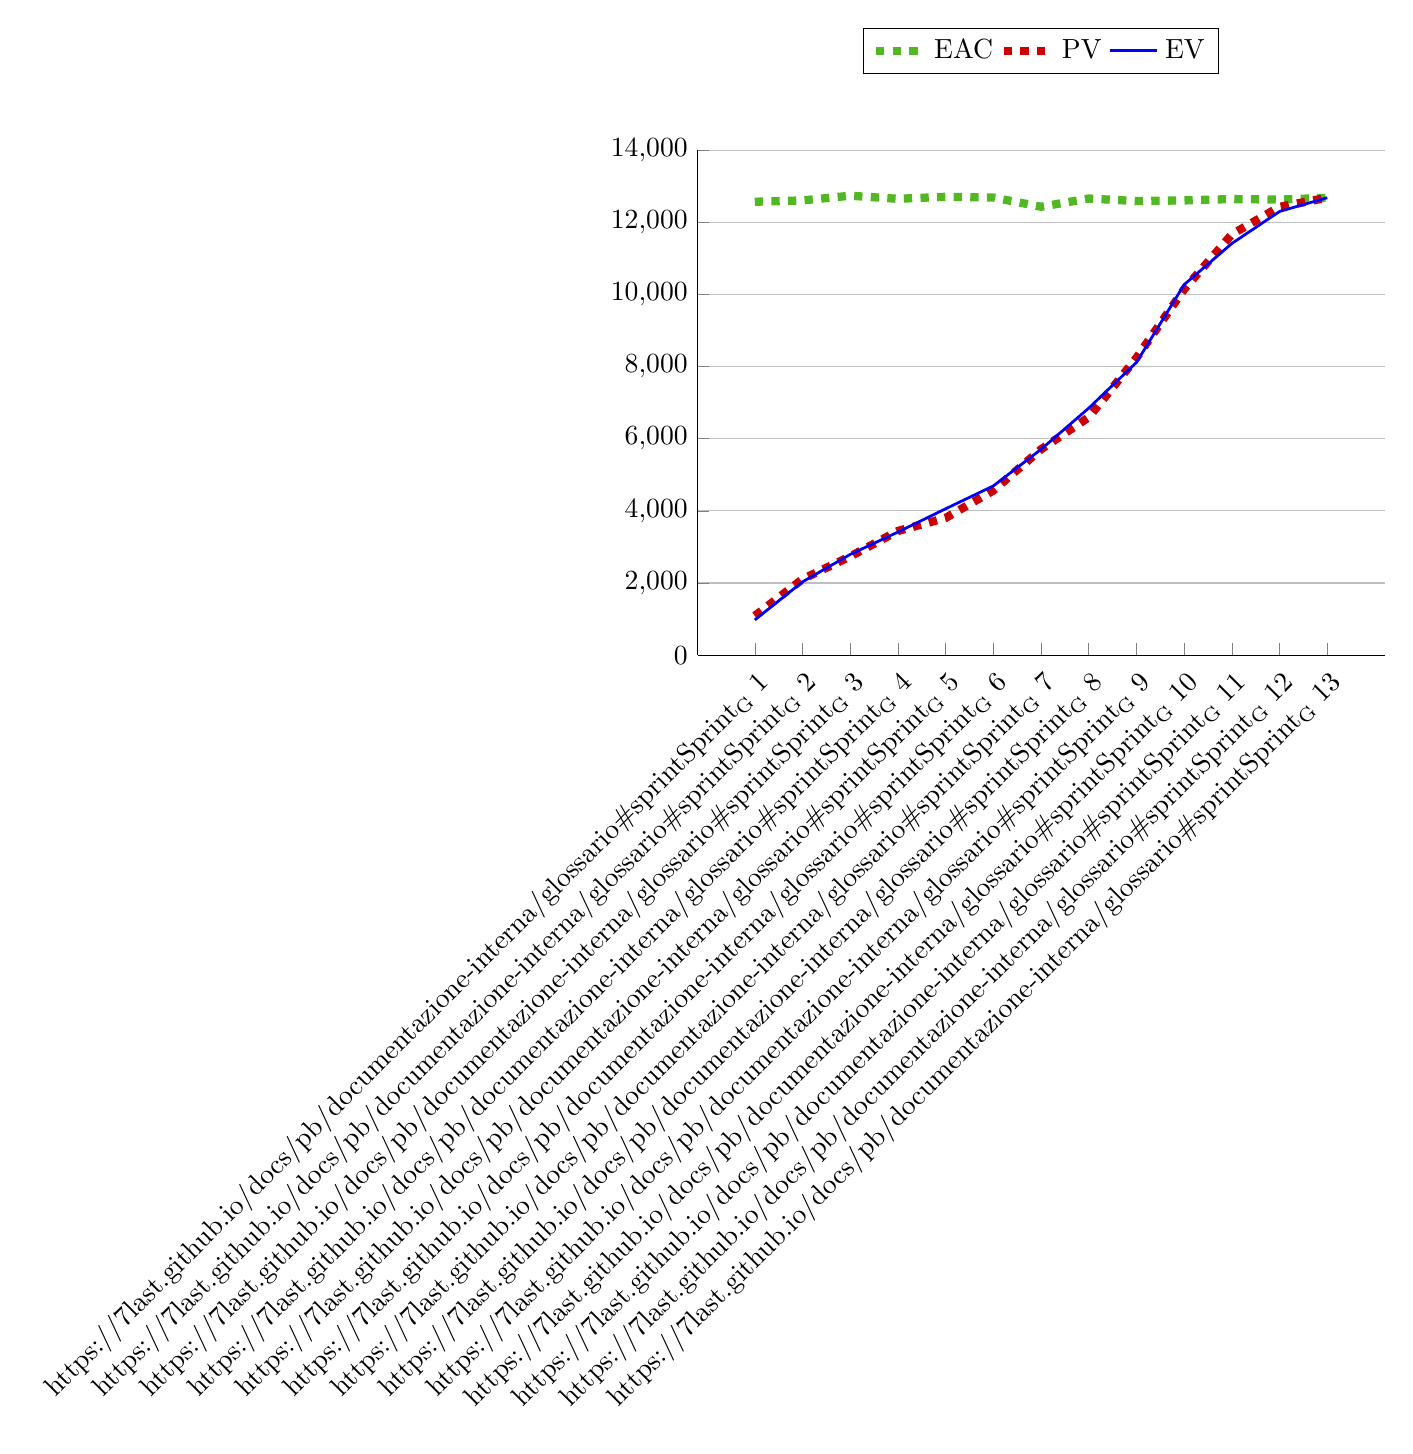
\begin{tikzpicture}
        \begin{axis}[
            width  = 0.85*\textwidth,
            height = 8cm,
            ymajorgrids = true,
            symbolic x coords={\href{https://7last.github.io/docs/pb/documentazione-interna/glossario\#sprint}{Sprint\textsubscript{G}} 1, \href{https://7last.github.io/docs/pb/documentazione-interna/glossario\#sprint}{Sprint\textsubscript{G}} 2, \href{https://7last.github.io/docs/pb/documentazione-interna/glossario\#sprint}{Sprint\textsubscript{G}} 3, \href{https://7last.github.io/docs/pb/documentazione-interna/glossario\#sprint}{Sprint\textsubscript{G}} 4, \href{https://7last.github.io/docs/pb/documentazione-interna/glossario\#sprint}{Sprint\textsubscript{G}} 5, \href{https://7last.github.io/docs/pb/documentazione-interna/glossario\#sprint}{Sprint\textsubscript{G}} 6, \href{https://7last.github.io/docs/pb/documentazione-interna/glossario\#sprint}{Sprint\textsubscript{G}} 7, \href{https://7last.github.io/docs/pb/documentazione-interna/glossario\#sprint}{Sprint\textsubscript{G}} 8, \href{https://7last.github.io/docs/pb/documentazione-interna/glossario\#sprint}{Sprint\textsubscript{G}} 9, \href{https://7last.github.io/docs/pb/documentazione-interna/glossario\#sprint}{Sprint\textsubscript{G}} 10, \href{https://7last.github.io/docs/pb/documentazione-interna/glossario\#sprint}{Sprint\textsubscript{G}} 11, \href{https://7last.github.io/docs/pb/documentazione-interna/glossario\#sprint}{Sprint\textsubscript{G}} 12, \href{https://7last.github.io/docs/pb/documentazione-interna/glossario\#sprint}{Sprint\textsubscript{G}} 13},
            xtick = data,
            ymin=0,
            axis lines*=left,
            legend cell align=left,
            legend style={
                at={(0.5,1.15)},
                anchor=south,
                column sep=0.1ex,
                legend columns=3
            },
            xticklabel style={rotate=45, anchor=north east, yshift=0ex, xshift=0ex},
            scaled y ticks = false,
            yticklabel style={/pgf/number format/fixed}
        ]
            \addplot[color=opt, style={dashed, line width=3pt}, mark=none] coordinates { % EAC
                (\href{https://7last.github.io/docs/pb/documentazione-interna/glossario\#sprint}{Sprint\textsubscript{G}} 1, 12567.5)
                (\href{https://7last.github.io/docs/pb/documentazione-interna/glossario\#sprint}{Sprint\textsubscript{G}} 2, 12605)
                (\href{https://7last.github.io/docs/pb/documentazione-interna/glossario\#sprint}{Sprint\textsubscript{G}} 3, 12735)
                (\href{https://7last.github.io/docs/pb/documentazione-interna/glossario\#sprint}{Sprint\textsubscript{G}} 4, 12650)
                (\href{https://7last.github.io/docs/pb/documentazione-interna/glossario\#sprint}{Sprint\textsubscript{G}} 5, 12705)
                (\href{https://7last.github.io/docs/pb/documentazione-interna/glossario\#sprint}{Sprint\textsubscript{G}} 6, 12685)
                (\href{https://7last.github.io/docs/pb/documentazione-interna/glossario\#sprint}{Sprint\textsubscript{G}} 7, 12430)
                (\href{https://7last.github.io/docs/pb/documentazione-interna/glossario\#sprint}{Sprint\textsubscript{G}} 8, 12657.5)
                (\href{https://7last.github.io/docs/pb/documentazione-interna/glossario\#sprint}{Sprint\textsubscript{G}} 9, 12587.5)
                (\href{https://7last.github.io/docs/pb/documentazione-interna/glossario\#sprint}{Sprint\textsubscript{G}} 10, 12605)
                (\href{https://7last.github.io/docs/pb/documentazione-interna/glossario\#sprint}{Sprint\textsubscript{G}} 11, 12642.5)
                (\href{https://7last.github.io/docs/pb/documentazione-interna/glossario\#sprint}{Sprint\textsubscript{G}} 12, 12627.5)
                (\href{https://7last.github.io/docs/pb/documentazione-interna/glossario\#sprint}{Sprint\textsubscript{G}} 13, 12677.5)
            };
            \addplot[color=amm, style={dashed, line width=3pt}, mark=none] coordinates { % PV
                (\href{https://7last.github.io/docs/pb/documentazione-interna/glossario\#sprint}{Sprint\textsubscript{G}} 1, 1090)
                (\href{https://7last.github.io/docs/pb/documentazione-interna/glossario\#sprint}{Sprint\textsubscript{G}} 2, 2107.5)
                (\href{https://7last.github.io/docs/pb/documentazione-interna/glossario\#sprint}{Sprint\textsubscript{G}} 3, 2737.5)
                (\href{https://7last.github.io/docs/pb/documentazione-interna/glossario\#sprint}{Sprint\textsubscript{G}} 4, 3442.5)
                (\href{https://7last.github.io/docs/pb/documentazione-interna/glossario\#sprint}{Sprint\textsubscript{G}} 5, 3804)
                (\href{https://7last.github.io/docs/pb/documentazione-interna/glossario\#sprint}{Sprint\textsubscript{G}} 6, 4564.8)
                (\href{https://7last.github.io/docs/pb/documentazione-interna/glossario\#sprint}{Sprint\textsubscript{G}} 7, 5706)
                (\href{https://7last.github.io/docs/pb/documentazione-interna/glossario\#sprint}{Sprint\textsubscript{G}} 8, 6593.6)
                (\href{https://7last.github.io/docs/pb/documentazione-interna/glossario\#sprint}{Sprint\textsubscript{G}} 9, 8242)
                (\href{https://7last.github.io/docs/pb/documentazione-interna/glossario\#sprint}{Sprint\textsubscript{G}} 10, 10144)
                (\href{https://7last.github.io/docs/pb/documentazione-interna/glossario\#sprint}{Sprint\textsubscript{G}} 11, 11665.6)
                (\href{https://7last.github.io/docs/pb/documentazione-interna/glossario\#sprint}{Sprint\textsubscript{G}} 12, 12426.4)
                (\href{https://7last.github.io/docs/pb/documentazione-interna/glossario\#sprint}{Sprint\textsubscript{G}} 13, 12680)
            };
            \addplot[color=blue, style={line width=1pt}, mark=none] coordinates { % EV
                (\href{https://7last.github.io/docs/pb/documentazione-interna/glossario\#sprint}{Sprint\textsubscript{G}} 1, 977.5)
                (\href{https://7last.github.io/docs/pb/documentazione-interna/glossario\#sprint}{Sprint\textsubscript{G}} 2, 2032.5)
                (\href{https://7last.github.io/docs/pb/documentazione-interna/glossario\#sprint}{Sprint\textsubscript{G}} 3, 2792.5)
                (\href{https://7last.github.io/docs/pb/documentazione-interna/glossario\#sprint}{Sprint\textsubscript{G}} 4, 3412.5)
                (\href{https://7last.github.io/docs/pb/documentazione-interna/glossario\#sprint}{Sprint\textsubscript{G}} 5, 4057.6)
                (\href{https://7last.github.io/docs/pb/documentazione-interna/glossario\#sprint}{Sprint\textsubscript{G}} 6, 4691.6)
                (\href{https://7last.github.io/docs/pb/documentazione-interna/glossario\#sprint}{Sprint\textsubscript{G}} 7, 5706)
                (\href{https://7last.github.io/docs/pb/documentazione-interna/glossario\#sprint}{Sprint\textsubscript{G}} 8, 6847.2)
                (\href{https://7last.github.io/docs/pb/documentazione-interna/glossario\#sprint}{Sprint\textsubscript{G}} 9, 8115.2)
                (\href{https://7last.github.io/docs/pb/documentazione-interna/glossario\#sprint}{Sprint\textsubscript{G}} 10, 10270.8)
                (\href{https://7last.github.io/docs/pb/documentazione-interna/glossario\#sprint}{Sprint\textsubscript{G}} 11, 11412)
                (\href{https://7last.github.io/docs/pb/documentazione-interna/glossario\#sprint}{Sprint\textsubscript{G}} 12, 12299.6)
                (\href{https://7last.github.io/docs/pb/documentazione-interna/glossario\#sprint}{Sprint\textsubscript{G}} 13, 12680)
            };
            \legend{EAC, PV, EV}
        \end{axis}
    \end{tikzpicture}
    \caption{Proiezione del PV e dell'EV}
\end{figure*}
%--------- FINE GRAFICO -----------%

\begin{flushleft}
\href{https://7last.github.io/docs/pb/documentazione-interna/glossario\#requirements-and-technology-baseline}{\textbf{RTB}\textsubscript{G}} \\
Visionando il grafico si può notare che i valori di EV e PV quasi si sovrappongono, questo indica la buona riuscita della pianificazione delle attività da parte del gruppo \textit{7Last}. \\
\href{https://7last.github.io/docs/pb/documentazione-interna/glossario\#product-baseline}{\textbf{PB}\textsubscript{G}} \\
Dal grafico completo si evince che il gruppo ha svolto le attività in modo efficiente, con un'evoluzione costante e in linea con la pianificazione. Questo è supportato dal fatto che i valori di EV e PV sono molto vicini tra loro, indicando che il gruppo ha pianificato correttamente le attività, confermando l'andamento positivo del progetto.
\end{flushleft}
    
\newpage
\subsubsection{3M-AC - Actual cost  e 9M-ETC - Estimate to complete}
%--------- GRAFICO -----------%
\begin{figure*}[!h]
    \centering
    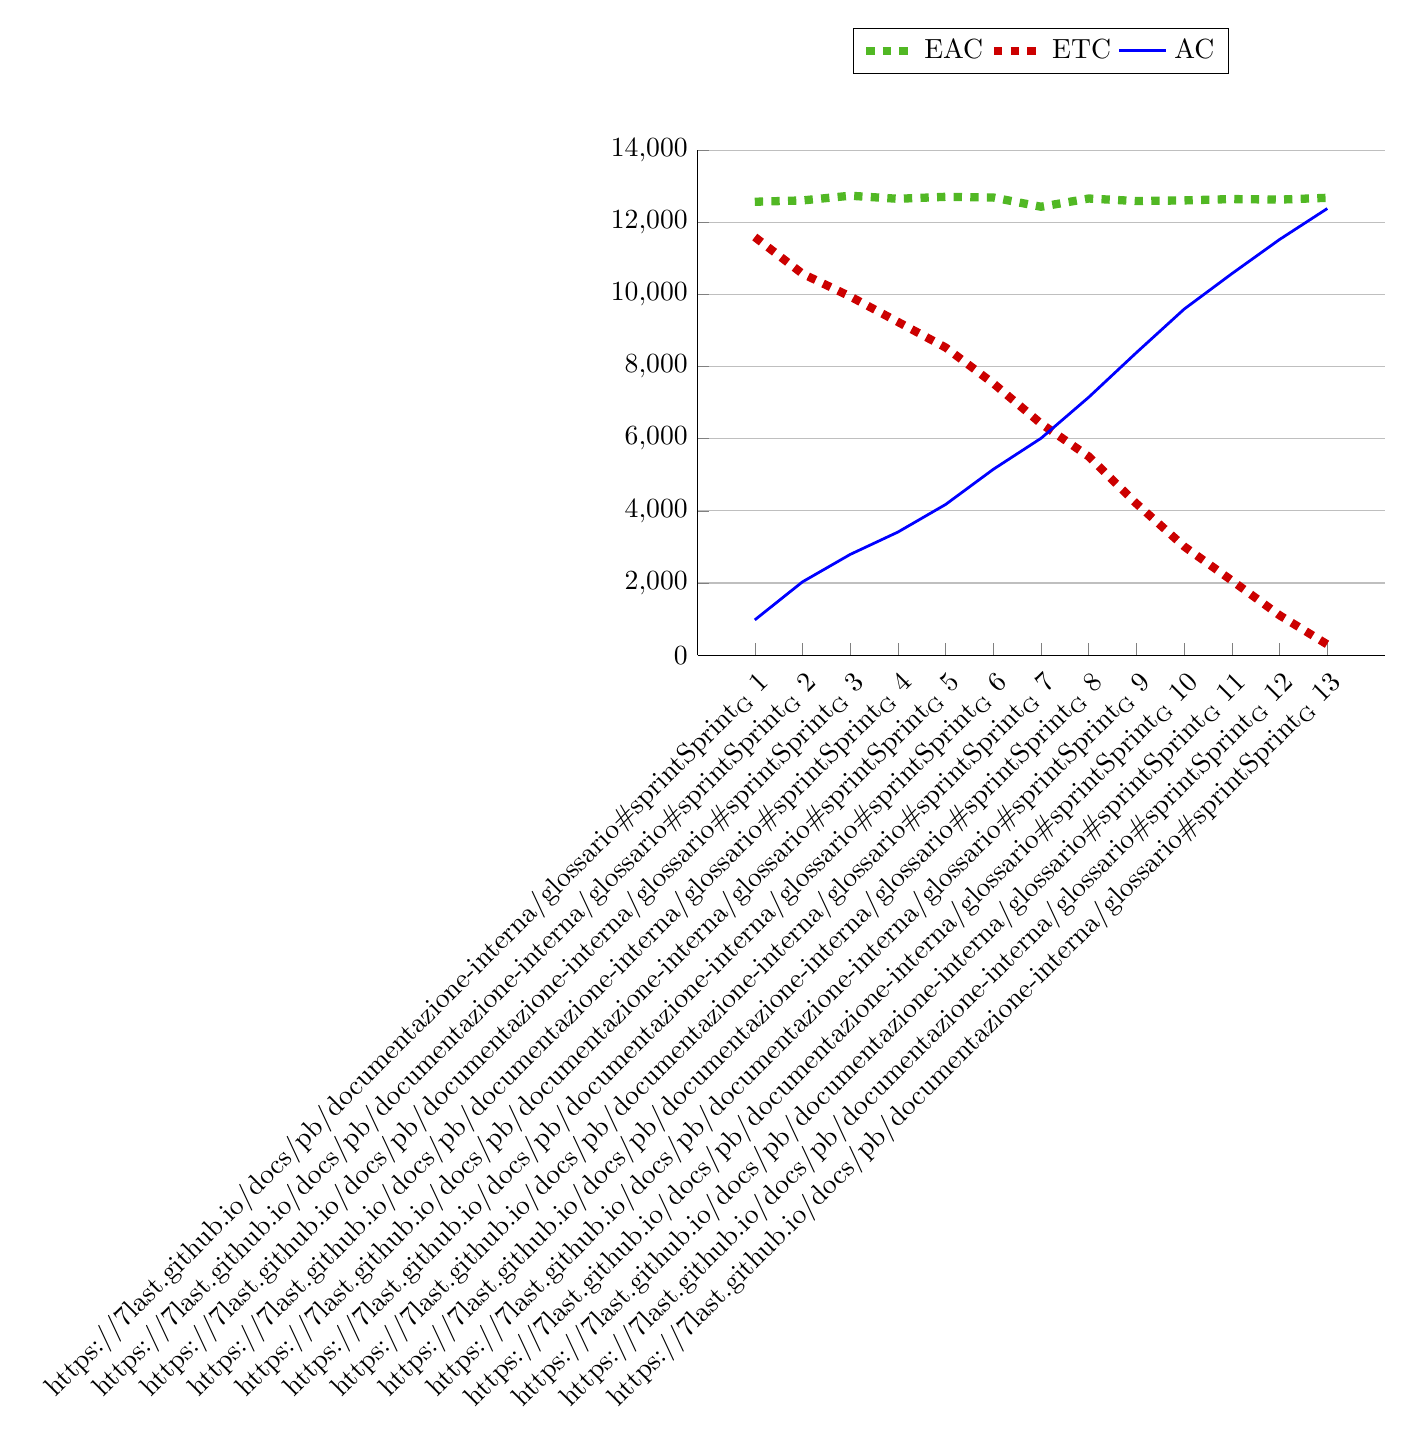
\begin{tikzpicture}
        \begin{axis}[
            width  = 0.85*\textwidth,
            height = 8cm,
            ymajorgrids = true,
            symbolic x coords={\href{https://7last.github.io/docs/pb/documentazione-interna/glossario\#sprint}{Sprint\textsubscript{G}} 1, \href{https://7last.github.io/docs/pb/documentazione-interna/glossario\#sprint}{Sprint\textsubscript{G}} 2, \href{https://7last.github.io/docs/pb/documentazione-interna/glossario\#sprint}{Sprint\textsubscript{G}} 3, \href{https://7last.github.io/docs/pb/documentazione-interna/glossario\#sprint}{Sprint\textsubscript{G}} 4, \href{https://7last.github.io/docs/pb/documentazione-interna/glossario\#sprint}{Sprint\textsubscript{G}} 5, \href{https://7last.github.io/docs/pb/documentazione-interna/glossario\#sprint}{Sprint\textsubscript{G}} 6, \href{https://7last.github.io/docs/pb/documentazione-interna/glossario\#sprint}{Sprint\textsubscript{G}} 7, \href{https://7last.github.io/docs/pb/documentazione-interna/glossario\#sprint}{Sprint\textsubscript{G}} 8, \href{https://7last.github.io/docs/pb/documentazione-interna/glossario\#sprint}{Sprint\textsubscript{G}} 9, \href{https://7last.github.io/docs/pb/documentazione-interna/glossario\#sprint}{Sprint\textsubscript{G}} 10, \href{https://7last.github.io/docs/pb/documentazione-interna/glossario\#sprint}{Sprint\textsubscript{G}} 11, \href{https://7last.github.io/docs/pb/documentazione-interna/glossario\#sprint}{Sprint\textsubscript{G}} 12, \href{https://7last.github.io/docs/pb/documentazione-interna/glossario\#sprint}{Sprint\textsubscript{G}} 13},
            xtick = data,
            ymin=0,
            axis lines*=left,
            legend cell align=left,
            legend style={
                at={(0.5,1.15)},
                anchor=south,
                column sep=0.1ex,
                legend columns=3
            },
            xticklabel style={rotate=45, anchor=north east, yshift=0ex, xshift=0ex},
            scaled y ticks = false,
            yticklabel style={/pgf/number format/fixed}
        ]
            \addplot[color=opt, style={dashed, line width=3pt}, mark=none] coordinates { % EAC
                (\href{https://7last.github.io/docs/pb/documentazione-interna/glossario\#sprint}{Sprint\textsubscript{G}} 1, 12567.5)
                (\href{https://7last.github.io/docs/pb/documentazione-interna/glossario\#sprint}{Sprint\textsubscript{G}} 2, 12605)
                (\href{https://7last.github.io/docs/pb/documentazione-interna/glossario\#sprint}{Sprint\textsubscript{G}} 3, 12735)
                (\href{https://7last.github.io/docs/pb/documentazione-interna/glossario\#sprint}{Sprint\textsubscript{G}} 4, 12650)
                (\href{https://7last.github.io/docs/pb/documentazione-interna/glossario\#sprint}{Sprint\textsubscript{G}} 5, 12705)
                (\href{https://7last.github.io/docs/pb/documentazione-interna/glossario\#sprint}{Sprint\textsubscript{G}} 6, 12685)
                (\href{https://7last.github.io/docs/pb/documentazione-interna/glossario\#sprint}{Sprint\textsubscript{G}} 7, 12430)
                (\href{https://7last.github.io/docs/pb/documentazione-interna/glossario\#sprint}{Sprint\textsubscript{G}} 8, 12657.5)
                (\href{https://7last.github.io/docs/pb/documentazione-interna/glossario\#sprint}{Sprint\textsubscript{G}} 9, 12587.5)
                (\href{https://7last.github.io/docs/pb/documentazione-interna/glossario\#sprint}{Sprint\textsubscript{G}} 10, 12605)
                (\href{https://7last.github.io/docs/pb/documentazione-interna/glossario\#sprint}{Sprint\textsubscript{G}} 11, 12642.5)
                (\href{https://7last.github.io/docs/pb/documentazione-interna/glossario\#sprint}{Sprint\textsubscript{G}} 12, 12627.5)
                (\href{https://7last.github.io/docs/pb/documentazione-interna/glossario\#sprint}{Sprint\textsubscript{G}} 13, 12677.5)
            };
            \addplot[color=amm, style={dashed, line width=3pt}, mark=none] coordinates { % ETC
                (\href{https://7last.github.io/docs/pb/documentazione-interna/glossario\#sprint}{Sprint\textsubscript{G}} 1, 11590)
                (\href{https://7last.github.io/docs/pb/documentazione-interna/glossario\#sprint}{Sprint\textsubscript{G}} 2, 10572.5)
                (\href{https://7last.github.io/docs/pb/documentazione-interna/glossario\#sprint}{Sprint\textsubscript{G}} 3, 9942.5)
                (\href{https://7last.github.io/docs/pb/documentazione-interna/glossario\#sprint}{Sprint\textsubscript{G}} 4, 9237.5)
                (\href{https://7last.github.io/docs/pb/documentazione-interna/glossario\#sprint}{Sprint\textsubscript{G}} 5, 8527.5)
                (\href{https://7last.github.io/docs/pb/documentazione-interna/glossario\#sprint}{Sprint\textsubscript{G}} 6, 7532.5)
                (\href{https://7last.github.io/docs/pb/documentazione-interna/glossario\#sprint}{Sprint\textsubscript{G}} 7, 6417.5)
                (\href{https://7last.github.io/docs/pb/documentazione-interna/glossario\#sprint}{Sprint\textsubscript{G}} 8, 5507.5)
                (\href{https://7last.github.io/docs/pb/documentazione-interna/glossario\#sprint}{Sprint\textsubscript{G}} 9, 4200)
                (\href{https://7last.github.io/docs/pb/documentazione-interna/glossario\#sprint}{Sprint\textsubscript{G}} 10, 3012.5)
                (\href{https://7last.github.io/docs/pb/documentazione-interna/glossario\#sprint}{Sprint\textsubscript{G}} 11, 2067.5)
                (\href{https://7last.github.io/docs/pb/documentazione-interna/glossario\#sprint}{Sprint\textsubscript{G}} 12, 1105)
                (\href{https://7last.github.io/docs/pb/documentazione-interna/glossario\#sprint}{Sprint\textsubscript{G}} 13, 297.5)
            };
            \addplot[color=blue, style={line width=1pt}, mark=none] coordinates { % AC
                (\href{https://7last.github.io/docs/pb/documentazione-interna/glossario\#sprint}{Sprint\textsubscript{G}} 1, 977.5)
                (\href{https://7last.github.io/docs/pb/documentazione-interna/glossario\#sprint}{Sprint\textsubscript{G}} 2, 2032.5)
                (\href{https://7last.github.io/docs/pb/documentazione-interna/glossario\#sprint}{Sprint\textsubscript{G}} 3, 2792.5)
                (\href{https://7last.github.io/docs/pb/documentazione-interna/glossario\#sprint}{Sprint\textsubscript{G}} 4, 3412.5)
                (\href{https://7last.github.io/docs/pb/documentazione-interna/glossario\#sprint}{Sprint\textsubscript{G}} 5, 4177.5)
                (\href{https://7last.github.io/docs/pb/documentazione-interna/glossario\#sprint}{Sprint\textsubscript{G}} 6, 5152.5)
                (\href{https://7last.github.io/docs/pb/documentazione-interna/glossario\#sprint}{Sprint\textsubscript{G}} 7, 6012.5)
                (\href{https://7last.github.io/docs/pb/documentazione-interna/glossario\#sprint}{Sprint\textsubscript{G}} 8, 7150)
                (\href{https://7last.github.io/docs/pb/documentazione-interna/glossario\#sprint}{Sprint\textsubscript{G}} 9, 8387.5)
                (\href{https://7last.github.io/docs/pb/documentazione-interna/glossario\#sprint}{Sprint\textsubscript{G}} 10, 9592.5)
                (\href{https://7last.github.io/docs/pb/documentazione-interna/glossario\#sprint}{Sprint\textsubscript{G}} 11, 10575)
                (\href{https://7last.github.io/docs/pb/documentazione-interna/glossario\#sprint}{Sprint\textsubscript{G}} 12, 11522.5)
                (\href{https://7last.github.io/docs/pb/documentazione-interna/glossario\#sprint}{Sprint\textsubscript{G}} 13, 12380)
            };
            \legend{EAC, ETC, AC}
        \end{axis}
    \end{tikzpicture}
    \caption{Proiezione dell'AC e dell'ETC}
\end{figure*}
%--------- FINE GRAFICO -----------%

\begin{flushleft}
\href{https://7last.github.io/docs/pb/documentazione-interna/glossario\#requirements-and-technology-baseline}{\textbf{RTB}\textsubscript{G}} \\
Il grafico evidenzia chiaramente un aumento progressivo dei costi (AC). Parallelamente, si osserva una diminuzione della stima dei costi a finire (ETC), che sta calando in modo proporzionale all'incremento dei costi. \\
\href{https://7last.github.io/docs/pb/documentazione-interna/glossario\#product-baseline}{\textbf{PB}\textsubscript{G}} \\
In questo secondo periodo viene confermato l'andamento evidenziato in quello precedente, con i costi reali (AC) che aumentano in modo proporzionale alla diminuzione della stima dei costi a finire (ETC). Questo indica che il gruppo ha svolto le attività in modo efficiente, con un allineamento tra i costi reali e quelli preventivati.
\end{flushleft}

\newpage
\subsubsection{4M-SV - Schedule variance e 5M-CV - Cost variance}
%--------- GRAFICO -----------%
\begin{figure*}[!h]
    \centering
    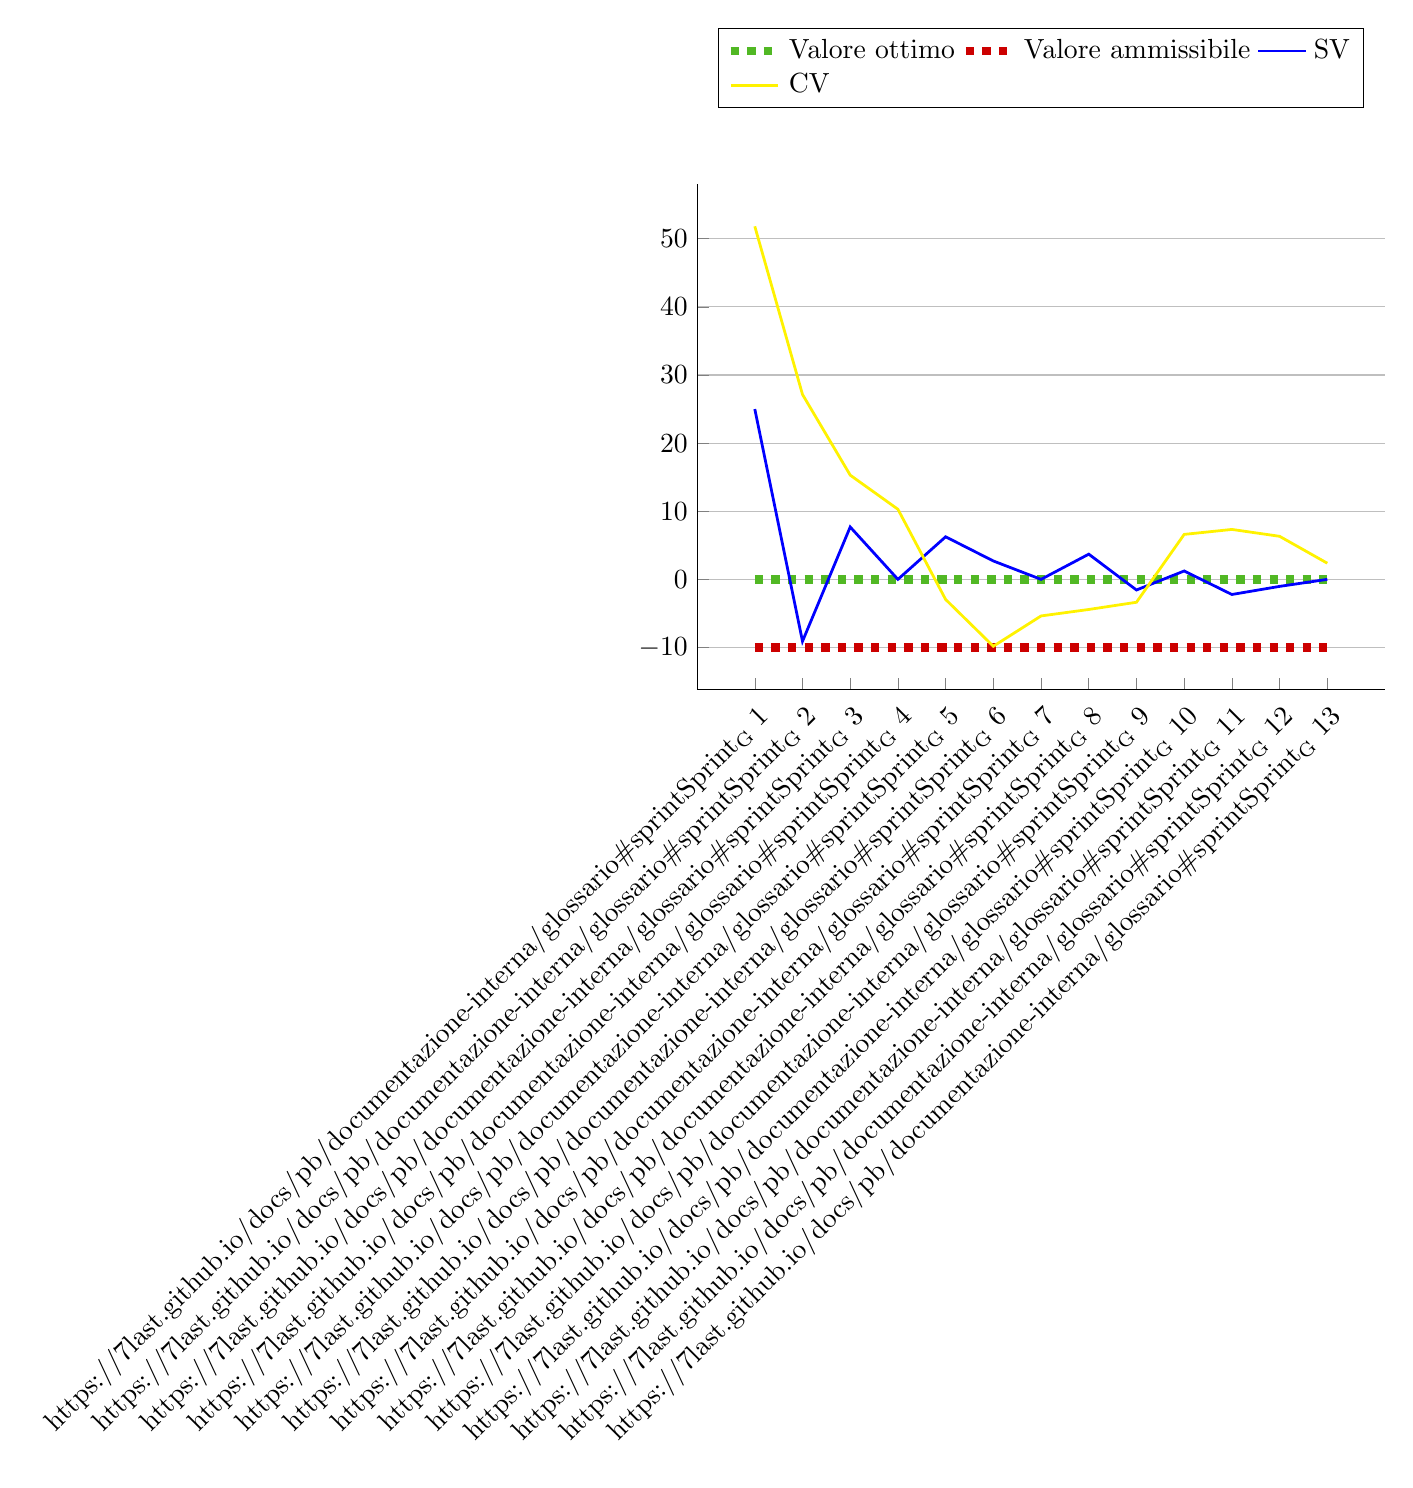
\begin{tikzpicture}
        \begin{axis}[
            width  = 0.85*\textwidth,
            height = 8cm,
            ymajorgrids = true,
            symbolic x coords={\href{https://7last.github.io/docs/pb/documentazione-interna/glossario\#sprint}{Sprint\textsubscript{G}} 1, \href{https://7last.github.io/docs/pb/documentazione-interna/glossario\#sprint}{Sprint\textsubscript{G}} 2, \href{https://7last.github.io/docs/pb/documentazione-interna/glossario\#sprint}{Sprint\textsubscript{G}} 3, \href{https://7last.github.io/docs/pb/documentazione-interna/glossario\#sprint}{Sprint\textsubscript{G}} 4, \href{https://7last.github.io/docs/pb/documentazione-interna/glossario\#sprint}{Sprint\textsubscript{G}} 5, \href{https://7last.github.io/docs/pb/documentazione-interna/glossario\#sprint}{Sprint\textsubscript{G}} 6, \href{https://7last.github.io/docs/pb/documentazione-interna/glossario\#sprint}{Sprint\textsubscript{G}} 7, \href{https://7last.github.io/docs/pb/documentazione-interna/glossario\#sprint}{Sprint\textsubscript{G}} 8, \href{https://7last.github.io/docs/pb/documentazione-interna/glossario\#sprint}{Sprint\textsubscript{G}} 9, \href{https://7last.github.io/docs/pb/documentazione-interna/glossario\#sprint}{Sprint\textsubscript{G}} 10, \href{https://7last.github.io/docs/pb/documentazione-interna/glossario\#sprint}{Sprint\textsubscript{G}} 11, \href{https://7last.github.io/docs/pb/documentazione-interna/glossario\#sprint}{Sprint\textsubscript{G}} 12, \href{https://7last.github.io/docs/pb/documentazione-interna/glossario\#sprint}{Sprint\textsubscript{G}} 13},
            xtick = data,
            axis lines*=left,
            legend cell align=left,
            legend style={
                at={(0.5,1.15)},
                anchor=south,
                column sep=0.1ex,
                legend columns=3
            },
            xticklabel style={rotate=45, anchor=north east, yshift=0ex, xshift=0ex}
        ]
            \addplot[color=opt, style={dashed, line width=3pt}, mark=none] coordinates { % ottimo = 0
                (\href{https://7last.github.io/docs/pb/documentazione-interna/glossario\#sprint}{Sprint\textsubscript{G}} 1, 0)
                (\href{https://7last.github.io/docs/pb/documentazione-interna/glossario\#sprint}{Sprint\textsubscript{G}} 2, 0)
                (\href{https://7last.github.io/docs/pb/documentazione-interna/glossario\#sprint}{Sprint\textsubscript{G}} 3, 0)
                (\href{https://7last.github.io/docs/pb/documentazione-interna/glossario\#sprint}{Sprint\textsubscript{G}} 4, 0)
                (\href{https://7last.github.io/docs/pb/documentazione-interna/glossario\#sprint}{Sprint\textsubscript{G}} 5, 0)
                (\href{https://7last.github.io/docs/pb/documentazione-interna/glossario\#sprint}{Sprint\textsubscript{G}} 6, 0)
                (\href{https://7last.github.io/docs/pb/documentazione-interna/glossario\#sprint}{Sprint\textsubscript{G}} 7, 0)
                (\href{https://7last.github.io/docs/pb/documentazione-interna/glossario\#sprint}{Sprint\textsubscript{G}} 8, 0)
                (\href{https://7last.github.io/docs/pb/documentazione-interna/glossario\#sprint}{Sprint\textsubscript{G}} 9, 0)
                (\href{https://7last.github.io/docs/pb/documentazione-interna/glossario\#sprint}{Sprint\textsubscript{G}} 10, 0)
                (\href{https://7last.github.io/docs/pb/documentazione-interna/glossario\#sprint}{Sprint\textsubscript{G}} 11, 0)
                (\href{https://7last.github.io/docs/pb/documentazione-interna/glossario\#sprint}{Sprint\textsubscript{G}} 12, 0)
                (\href{https://7last.github.io/docs/pb/documentazione-interna/glossario\#sprint}{Sprint\textsubscript{G}} 13, 0)
            };
            \addplot[color=amm, style={dashed, line width=3pt}, mark=none] coordinates { % ammissibile = -10
                (\href{https://7last.github.io/docs/pb/documentazione-interna/glossario\#sprint}{Sprint\textsubscript{G}} 1, -10)
                (\href{https://7last.github.io/docs/pb/documentazione-interna/glossario\#sprint}{Sprint\textsubscript{G}} 2, -10)
                (\href{https://7last.github.io/docs/pb/documentazione-interna/glossario\#sprint}{Sprint\textsubscript{G}} 3, -10)
                (\href{https://7last.github.io/docs/pb/documentazione-interna/glossario\#sprint}{Sprint\textsubscript{G}} 4, -10)
                (\href{https://7last.github.io/docs/pb/documentazione-interna/glossario\#sprint}{Sprint\textsubscript{G}} 5, -10)
                (\href{https://7last.github.io/docs/pb/documentazione-interna/glossario\#sprint}{Sprint\textsubscript{G}} 6, -10)
                (\href{https://7last.github.io/docs/pb/documentazione-interna/glossario\#sprint}{Sprint\textsubscript{G}} 7, -10)
                (\href{https://7last.github.io/docs/pb/documentazione-interna/glossario\#sprint}{Sprint\textsubscript{G}} 8, -10)
                (\href{https://7last.github.io/docs/pb/documentazione-interna/glossario\#sprint}{Sprint\textsubscript{G}} 9, -10)
                (\href{https://7last.github.io/docs/pb/documentazione-interna/glossario\#sprint}{Sprint\textsubscript{G}} 10, -10)
                (\href{https://7last.github.io/docs/pb/documentazione-interna/glossario\#sprint}{Sprint\textsubscript{G}} 11, -10)
                (\href{https://7last.github.io/docs/pb/documentazione-interna/glossario\#sprint}{Sprint\textsubscript{G}} 12, -10)
                (\href{https://7last.github.io/docs/pb/documentazione-interna/glossario\#sprint}{Sprint\textsubscript{G}} 13, -10)
            };
            \addplot[color=blue, style={line width=1pt}, mark=none] coordinates { % SV
                (\href{https://7last.github.io/docs/pb/documentazione-interna/glossario\#sprint}{Sprint\textsubscript{G}} 1, 25)
                (\href{https://7last.github.io/docs/pb/documentazione-interna/glossario\#sprint}{Sprint\textsubscript{G}} 2, -9.09)
                (\href{https://7last.github.io/docs/pb/documentazione-interna/glossario\#sprint}{Sprint\textsubscript{G}} 3, 7.69)
                (\href{https://7last.github.io/docs/pb/documentazione-interna/glossario\#sprint}{Sprint\textsubscript{G}} 4, 0)
                (\href{https://7last.github.io/docs/pb/documentazione-interna/glossario\#sprint}{Sprint\textsubscript{G}} 5, 6.25)
                (\href{https://7last.github.io/docs/pb/documentazione-interna/glossario\#sprint}{Sprint\textsubscript{G}} 6, 2.7)
                (\href{https://7last.github.io/docs/pb/documentazione-interna/glossario\#sprint}{Sprint\textsubscript{G}} 7, 0)
                (\href{https://7last.github.io/docs/pb/documentazione-interna/glossario\#sprint}{Sprint\textsubscript{G}} 8, 3.7)
                (\href{https://7last.github.io/docs/pb/documentazione-interna/glossario\#sprint}{Sprint\textsubscript{G}} 9, -1.56)
                (\href{https://7last.github.io/docs/pb/documentazione-interna/glossario\#sprint}{Sprint\textsubscript{G}} 10, 1.23)
                (\href{https://7last.github.io/docs/pb/documentazione-interna/glossario\#sprint}{Sprint\textsubscript{G}} 11, -2.22)
                (\href{https://7last.github.io/docs/pb/documentazione-interna/glossario\#sprint}{Sprint\textsubscript{G}} 12, -1.03)
                (\href{https://7last.github.io/docs/pb/documentazione-interna/glossario\#sprint}{Sprint\textsubscript{G}} 13, 0)
            };
            \addplot[color=yellow, style={line width=1pt}, mark=none] coordinates { % CV
                (\href{https://7last.github.io/docs/pb/documentazione-interna/glossario\#sprint}{Sprint\textsubscript{G}} 1, 51.82)
                (\href{https://7last.github.io/docs/pb/documentazione-interna/glossario\#sprint}{Sprint\textsubscript{G}} 2, 27.14)
                (\href{https://7last.github.io/docs/pb/documentazione-interna/glossario\#sprint}{Sprint\textsubscript{G}} 3, 15.30)
                (\href{https://7last.github.io/docs/pb/documentazione-interna/glossario\#sprint}{Sprint\textsubscript{G}} 4, 10.29)
                (\href{https://7last.github.io/docs/pb/documentazione-interna/glossario\#sprint}{Sprint\textsubscript{G}} 5, -2.95)
                (\href{https://7last.github.io/docs/pb/documentazione-interna/glossario\#sprint}{Sprint\textsubscript{G}} 6, -9.82)
                (\href{https://7last.github.io/docs/pb/documentazione-interna/glossario\#sprint}{Sprint\textsubscript{G}} 7, -5.37)
                (\href{https://7last.github.io/docs/pb/documentazione-interna/glossario\#sprint}{Sprint\textsubscript{G}} 8, -4.42)
                (\href{https://7last.github.io/docs/pb/documentazione-interna/glossario\#sprint}{Sprint\textsubscript{G}} 9, -3.36)
                (\href{https://7last.github.io/docs/pb/documentazione-interna/glossario\#sprint}{Sprint\textsubscript{G}} 10, 6.6)
                (\href{https://7last.github.io/docs/pb/documentazione-interna/glossario\#sprint}{Sprint\textsubscript{G}} 11, 7.33)
                (\href{https://7last.github.io/docs/pb/documentazione-interna/glossario\#sprint}{Sprint\textsubscript{G}} 12, 6.32)
                (\href{https://7last.github.io/docs/pb/documentazione-interna/glossario\#sprint}{Sprint\textsubscript{G}} 13, 2.37)
            };
            \legend{Valore ottimo, Valore ammissibile, SV, CV}
        \end{axis}
    \end{tikzpicture}
    \caption{Andamento percentuale di SV e CV}
\end{figure*}
%--------- FINE GRAFICO -----------%
\begin{flushleft}
\href{https://7last.github.io/docs/pb/documentazione-interna/glossario\#requirements-and-technology-baseline}{\textbf{RTB}\textsubscript{G}} \\
Dal grafico si nota come sia SV che CV siano inizialmente elevati, per poi decrescere durante la prosecuzione del progetto, in particolare si nota un andamento altalenante del SV. L'andamento inizialmente alto del Schedule Variance (SV) e del Cost Variance (CV) indica una possibile sovrastima iniziale dei tempi e dei costi, dovuta all'inesperienza del team. La variabilità del SV suggerisce che le stime di tempistiche iniziali erano eccessivamente conservative, con aggiustamenti successivi man mano che il team acquisiva esperienza. La decrescita nel tempo di entrambe le metriche mostra che il gruppo sta diventando più preciso nelle sue previsioni, con un allineamento progressivo dei costi e delle tempistiche reali rispetto a quelle pianificate. \\
\href{https://7last.github.io/docs/pb/documentazione-interna/glossario\#product-baseline}{\textbf{PB}\textsubscript{G}} \\
L'andamento del grafico nella seconda parte del progetto conferma il trend positivo iniziato nel periodo precedente, con SV e CV che si avvicinano ai valori ottimali.
\end{flushleft}

\newpage
\subsubsection{8M-EAC - Estimated at completion}
%--------- GRAFICO -----------%
\begin{figure*}[!h]
    \centering
    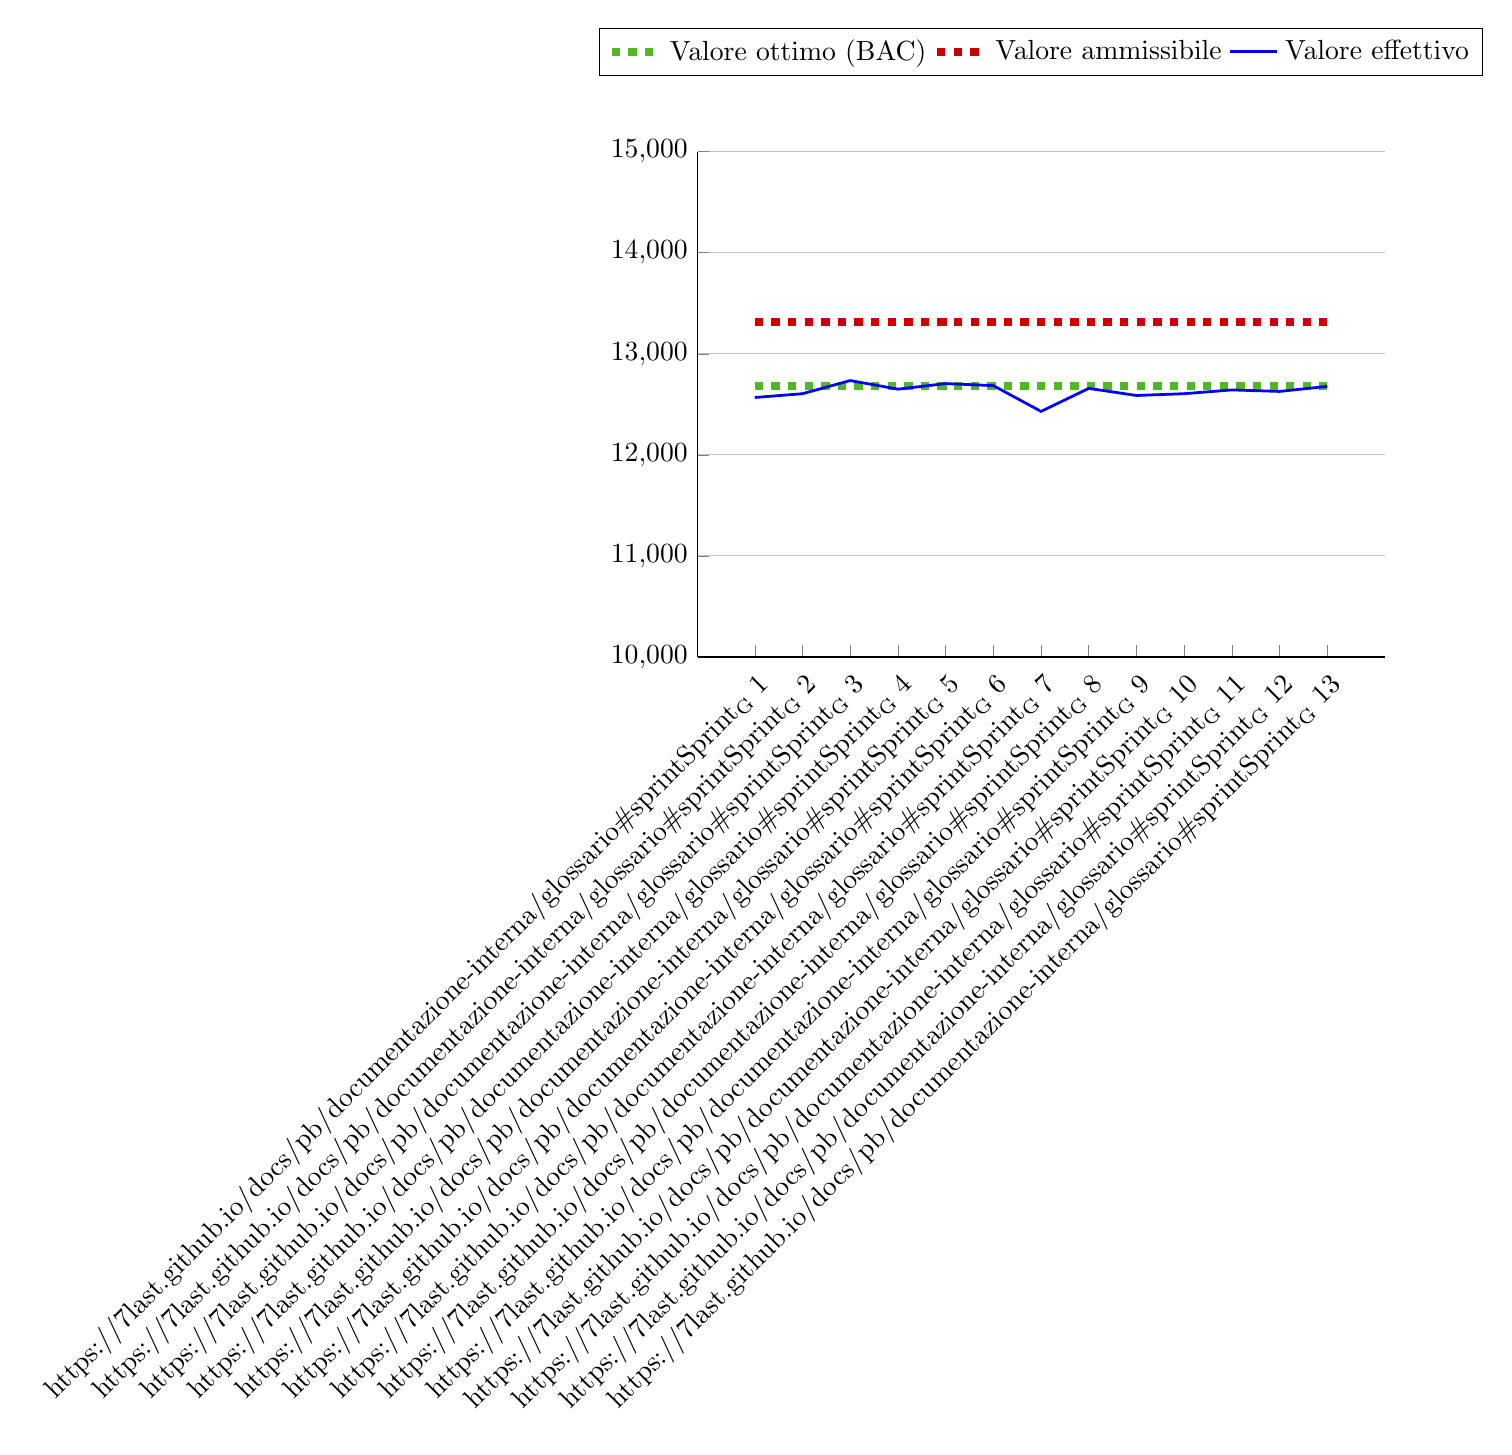
\begin{tikzpicture}
        \begin{axis}[
            width  = 0.85*\textwidth,
            height = 8cm,
            ymajorgrids = true,
            symbolic x coords={\href{https://7last.github.io/docs/pb/documentazione-interna/glossario\#sprint}{Sprint\textsubscript{G}} 1, \href{https://7last.github.io/docs/pb/documentazione-interna/glossario\#sprint}{Sprint\textsubscript{G}} 2, \href{https://7last.github.io/docs/pb/documentazione-interna/glossario\#sprint}{Sprint\textsubscript{G}} 3, \href{https://7last.github.io/docs/pb/documentazione-interna/glossario\#sprint}{Sprint\textsubscript{G}} 4, \href{https://7last.github.io/docs/pb/documentazione-interna/glossario\#sprint}{Sprint\textsubscript{G}} 5, \href{https://7last.github.io/docs/pb/documentazione-interna/glossario\#sprint}{Sprint\textsubscript{G}} 6, \href{https://7last.github.io/docs/pb/documentazione-interna/glossario\#sprint}{Sprint\textsubscript{G}} 7, \href{https://7last.github.io/docs/pb/documentazione-interna/glossario\#sprint}{Sprint\textsubscript{G}} 8, \href{https://7last.github.io/docs/pb/documentazione-interna/glossario\#sprint}{Sprint\textsubscript{G}} 9, \href{https://7last.github.io/docs/pb/documentazione-interna/glossario\#sprint}{Sprint\textsubscript{G}} 10, \href{https://7last.github.io/docs/pb/documentazione-interna/glossario\#sprint}{Sprint\textsubscript{G}} 11, \href{https://7last.github.io/docs/pb/documentazione-interna/glossario\#sprint}{Sprint\textsubscript{G}} 12, \href{https://7last.github.io/docs/pb/documentazione-interna/glossario\#sprint}{Sprint\textsubscript{G}} 13},
            xtick = data,
            ytick = {10000, 11000, 12000, 13000, 14000, 15000},
            ymin=10000, ymax=15000,
            axis lines*=left,
            legend cell align=left,
            legend style={
                at={(0.5,1.15)},
                anchor=south,
                column sep=0.1ex,
                legend columns=3
            },
            xticklabel style={rotate=45, anchor=north east, yshift=0ex, xshift=0ex},
            scaled y ticks = false,
            yticklabel style={/pgf/number format/fixed}
        ]
            \addplot[color=opt, style={dashed, line width=3pt}, mark=none] coordinates { % ottimo = BAC
                (\href{https://7last.github.io/docs/pb/documentazione-interna/glossario\#sprint}{Sprint\textsubscript{G}} 1, 12680)
                (\href{https://7last.github.io/docs/pb/documentazione-interna/glossario\#sprint}{Sprint\textsubscript{G}} 2, 12680)
                (\href{https://7last.github.io/docs/pb/documentazione-interna/glossario\#sprint}{Sprint\textsubscript{G}} 3, 12680)
                (\href{https://7last.github.io/docs/pb/documentazione-interna/glossario\#sprint}{Sprint\textsubscript{G}} 4, 12680)
                (\href{https://7last.github.io/docs/pb/documentazione-interna/glossario\#sprint}{Sprint\textsubscript{G}} 5, 12680)
                (\href{https://7last.github.io/docs/pb/documentazione-interna/glossario\#sprint}{Sprint\textsubscript{G}} 6, 12680)
                (\href{https://7last.github.io/docs/pb/documentazione-interna/glossario\#sprint}{Sprint\textsubscript{G}} 7, 12680)
                (\href{https://7last.github.io/docs/pb/documentazione-interna/glossario\#sprint}{Sprint\textsubscript{G}} 8, 12680)
                (\href{https://7last.github.io/docs/pb/documentazione-interna/glossario\#sprint}{Sprint\textsubscript{G}} 9, 12680)
                (\href{https://7last.github.io/docs/pb/documentazione-interna/glossario\#sprint}{Sprint\textsubscript{G}} 10, 12680)
                (\href{https://7last.github.io/docs/pb/documentazione-interna/glossario\#sprint}{Sprint\textsubscript{G}} 11, 12680)
                (\href{https://7last.github.io/docs/pb/documentazione-interna/glossario\#sprint}{Sprint\textsubscript{G}} 12, 12680)
                (\href{https://7last.github.io/docs/pb/documentazione-interna/glossario\#sprint}{Sprint\textsubscript{G}} 13, 12680)
            };
            \addplot[color=amm, style={dashed, line width=3pt}, mark=none] coordinates { % ammissibile = BAC + 5%
                (\href{https://7last.github.io/docs/pb/documentazione-interna/glossario\#sprint}{Sprint\textsubscript{G}} 1, 13314)
                (\href{https://7last.github.io/docs/pb/documentazione-interna/glossario\#sprint}{Sprint\textsubscript{G}} 2, 13314)
                (\href{https://7last.github.io/docs/pb/documentazione-interna/glossario\#sprint}{Sprint\textsubscript{G}} 3, 13314)
                (\href{https://7last.github.io/docs/pb/documentazione-interna/glossario\#sprint}{Sprint\textsubscript{G}} 4, 13314)
                (\href{https://7last.github.io/docs/pb/documentazione-interna/glossario\#sprint}{Sprint\textsubscript{G}} 5, 13314)
                (\href{https://7last.github.io/docs/pb/documentazione-interna/glossario\#sprint}{Sprint\textsubscript{G}} 6, 13314)
                (\href{https://7last.github.io/docs/pb/documentazione-interna/glossario\#sprint}{Sprint\textsubscript{G}} 7, 13314)
                (\href{https://7last.github.io/docs/pb/documentazione-interna/glossario\#sprint}{Sprint\textsubscript{G}} 8, 13314)
                (\href{https://7last.github.io/docs/pb/documentazione-interna/glossario\#sprint}{Sprint\textsubscript{G}} 9, 13314)
                (\href{https://7last.github.io/docs/pb/documentazione-interna/glossario\#sprint}{Sprint\textsubscript{G}} 10, 13314)
                (\href{https://7last.github.io/docs/pb/documentazione-interna/glossario\#sprint}{Sprint\textsubscript{G}} 11, 13314)
                (\href{https://7last.github.io/docs/pb/documentazione-interna/glossario\#sprint}{Sprint\textsubscript{G}} 12, 13314)
                (\href{https://7last.github.io/docs/pb/documentazione-interna/glossario\#sprint}{Sprint\textsubscript{G}} 13, 13314)
            };
            \addplot[color=blue, style={line width=1pt}, mark=none] coordinates { % EAC
                (\href{https://7last.github.io/docs/pb/documentazione-interna/glossario\#sprint}{Sprint\textsubscript{G}} 1, 12567.5)
                (\href{https://7last.github.io/docs/pb/documentazione-interna/glossario\#sprint}{Sprint\textsubscript{G}} 2, 12605)
                (\href{https://7last.github.io/docs/pb/documentazione-interna/glossario\#sprint}{Sprint\textsubscript{G}} 3, 12735)
                (\href{https://7last.github.io/docs/pb/documentazione-interna/glossario\#sprint}{Sprint\textsubscript{G}} 4, 12650)
                (\href{https://7last.github.io/docs/pb/documentazione-interna/glossario\#sprint}{Sprint\textsubscript{G}} 5, 12705)
                (\href{https://7last.github.io/docs/pb/documentazione-interna/glossario\#sprint}{Sprint\textsubscript{G}} 6, 12685)
                (\href{https://7last.github.io/docs/pb/documentazione-interna/glossario\#sprint}{Sprint\textsubscript{G}} 7, 12430)
                (\href{https://7last.github.io/docs/pb/documentazione-interna/glossario\#sprint}{Sprint\textsubscript{G}} 8, 12657.5)
                (\href{https://7last.github.io/docs/pb/documentazione-interna/glossario\#sprint}{Sprint\textsubscript{G}} 9, 12587.5)
                (\href{https://7last.github.io/docs/pb/documentazione-interna/glossario\#sprint}{Sprint\textsubscript{G}} 10, 12605)
                (\href{https://7last.github.io/docs/pb/documentazione-interna/glossario\#sprint}{Sprint\textsubscript{G}} 11, 12642.5)
                (\href{https://7last.github.io/docs/pb/documentazione-interna/glossario\#sprint}{Sprint\textsubscript{G}} 12, 12627.5)
                (\href{https://7last.github.io/docs/pb/documentazione-interna/glossario\#sprint}{Sprint\textsubscript{G}} 13, 12677.5)
            };
            \legend{Valore ottimo (BAC), Valore ammissibile, Valore effettivo}
        \end{axis}
    \end{tikzpicture}
    \caption{Proiezione dell'EAC}
\end{figure*}
%--------- FINE GRAFICO -----------%
\begin{flushleft}
\href{https://7last.github.io/docs/pb/documentazione-interna/glossario\#requirements-and-technology-baseline}{\textbf{RTB}\textsubscript{G}} \\
Osservando il grafico si può notare come l'EAC sia quasi sovrapposto al BAC durante i periodi di progetto analizzati fino ad ora. Questa situazione riflette come \textit{7Last} abbia attuato una gestione efficace sia dei costi che delle tempistiche durante i periodi analizzati fino ad ora. \\
\href{https://7last.github.io/docs/pb/documentazione-interna/glossario\#product-baseline}{\textbf{PB}\textsubscript{G}} \\
Anche in questo grafico abbiamo una conferma dell'andamento rilevato nella prima parte del progetto, con l'EAC che si mantiene costantemente vicino al BAC. Questo indica che il gruppo ha svolto le attività in modo efficiente, con un allineamento tra i costi reali e quelli preventivati, senza variazioni significative.
\end{flushleft}

\newpage
\subsection{Qualità del processo di analisi dei requisiti}
\subsubsection{11M-PRO - Percentuale requisiti obbligatori}
%--------- GRAFICO -----------%
\begin{figure*}[!h]
    \centering
    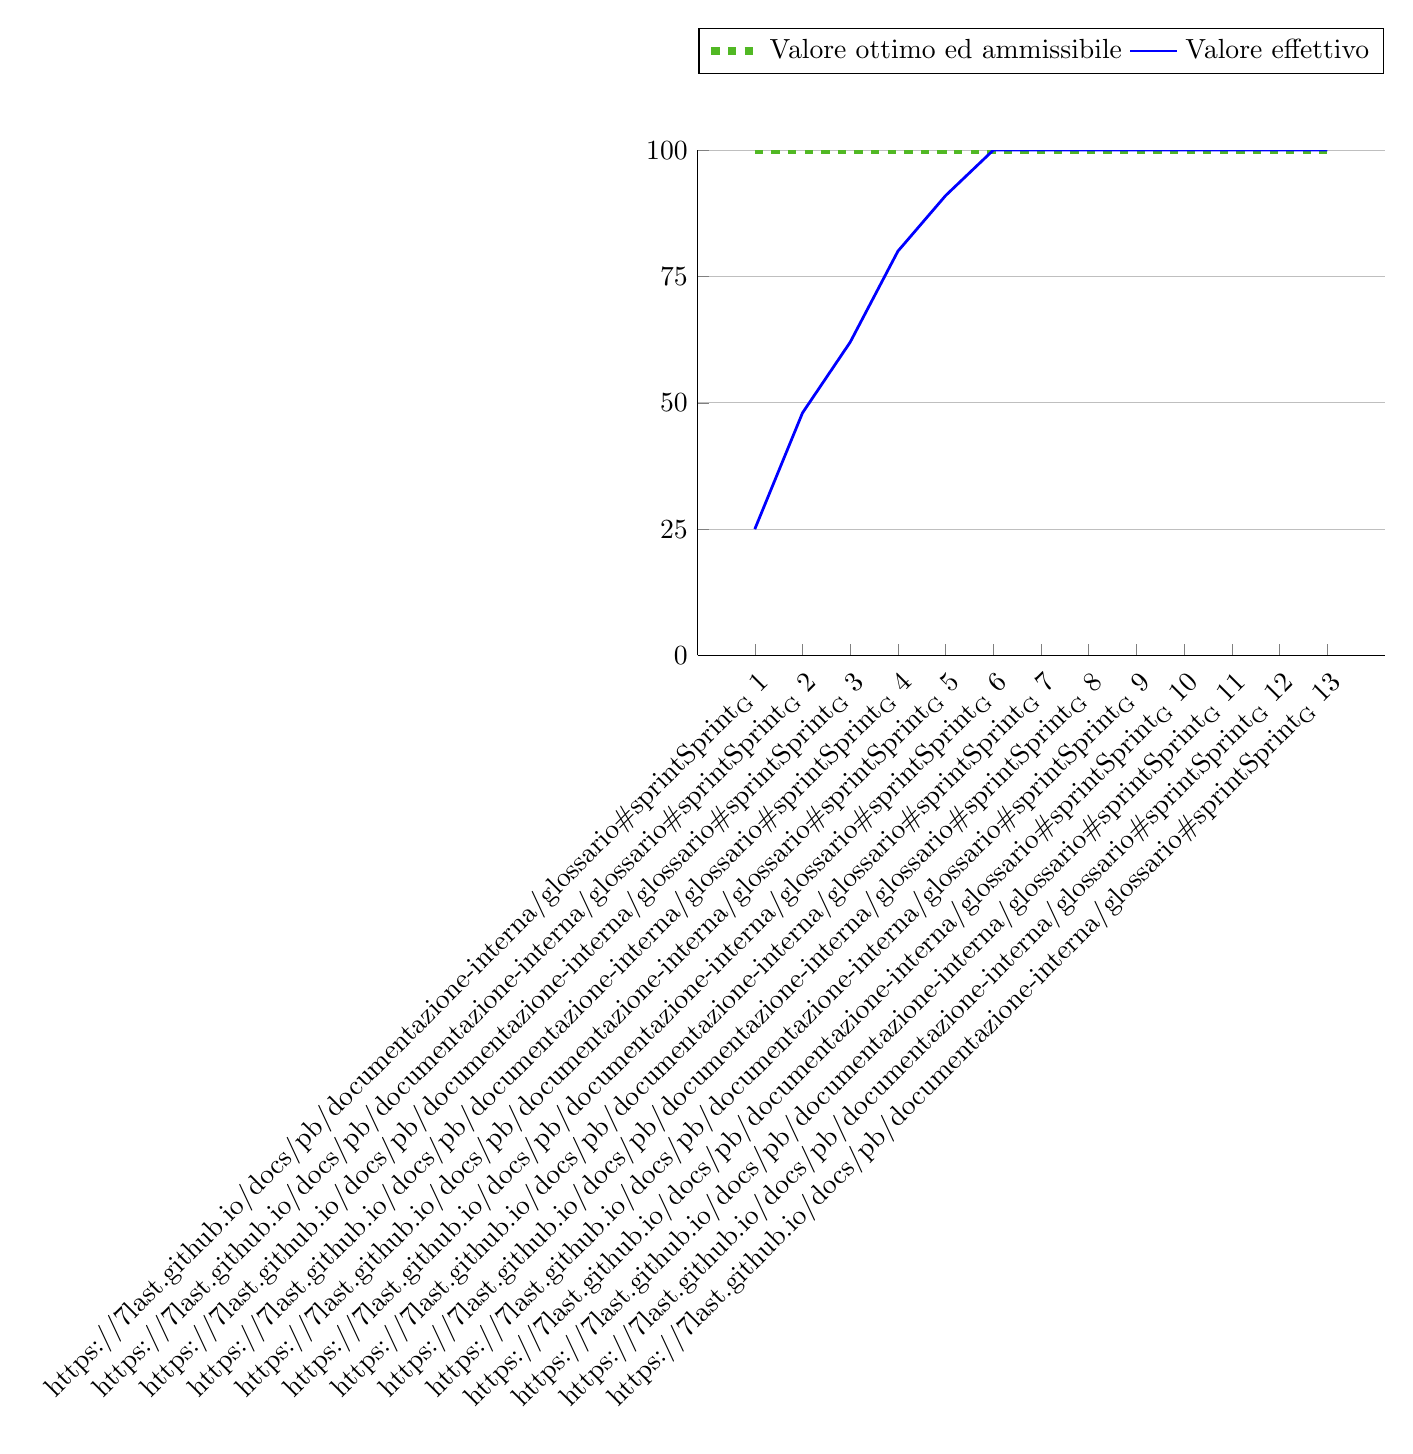
\begin{tikzpicture}
        \begin{axis}[
            width  = 0.85*\textwidth,
            height = 8cm,
            ymajorgrids = true,
            symbolic x coords={\href{https://7last.github.io/docs/pb/documentazione-interna/glossario\#sprint}{Sprint\textsubscript{G}} 1, \href{https://7last.github.io/docs/pb/documentazione-interna/glossario\#sprint}{Sprint\textsubscript{G}} 2, \href{https://7last.github.io/docs/pb/documentazione-interna/glossario\#sprint}{Sprint\textsubscript{G}} 3, \href{https://7last.github.io/docs/pb/documentazione-interna/glossario\#sprint}{Sprint\textsubscript{G}} 4, \href{https://7last.github.io/docs/pb/documentazione-interna/glossario\#sprint}{Sprint\textsubscript{G}} 5, \href{https://7last.github.io/docs/pb/documentazione-interna/glossario\#sprint}{Sprint\textsubscript{G}} 6, \href{https://7last.github.io/docs/pb/documentazione-interna/glossario\#sprint}{Sprint\textsubscript{G}} 7, \href{https://7last.github.io/docs/pb/documentazione-interna/glossario\#sprint}{Sprint\textsubscript{G}} 8, \href{https://7last.github.io/docs/pb/documentazione-interna/glossario\#sprint}{Sprint\textsubscript{G}} 9, \href{https://7last.github.io/docs/pb/documentazione-interna/glossario\#sprint}{Sprint\textsubscript{G}} 10, \href{https://7last.github.io/docs/pb/documentazione-interna/glossario\#sprint}{Sprint\textsubscript{G}} 11, \href{https://7last.github.io/docs/pb/documentazione-interna/glossario\#sprint}{Sprint\textsubscript{G}} 12, \href{https://7last.github.io/docs/pb/documentazione-interna/glossario\#sprint}{Sprint\textsubscript{G}} 13},
            xtick = data,
            ytick = {0, 25, 50, 75, 100},
            ymin=0, ymax=100,
            axis lines*=left,
            legend cell align=left,
            legend style={
                at={(0.5,1.15)},
                anchor=south,
                column sep=0.1ex,
                legend columns=3
            },
            xticklabel style={rotate=45, anchor=north east, yshift=0ex, xshift=0ex}
            ]
            \addplot[color=opt, style={dashed, line width=3pt}, mark=none] coordinates { % ottimo = 100
                (\href{https://7last.github.io/docs/pb/documentazione-interna/glossario\#sprint}{Sprint\textsubscript{G}} 1, 100)
                (\href{https://7last.github.io/docs/pb/documentazione-interna/glossario\#sprint}{Sprint\textsubscript{G}} 2, 100)
                (\href{https://7last.github.io/docs/pb/documentazione-interna/glossario\#sprint}{Sprint\textsubscript{G}} 3, 100)
                (\href{https://7last.github.io/docs/pb/documentazione-interna/glossario\#sprint}{Sprint\textsubscript{G}} 4, 100)
                (\href{https://7last.github.io/docs/pb/documentazione-interna/glossario\#sprint}{Sprint\textsubscript{G}} 5, 100)
                (\href{https://7last.github.io/docs/pb/documentazione-interna/glossario\#sprint}{Sprint\textsubscript{G}} 6, 100)
                (\href{https://7last.github.io/docs/pb/documentazione-interna/glossario\#sprint}{Sprint\textsubscript{G}} 7, 100)
                (\href{https://7last.github.io/docs/pb/documentazione-interna/glossario\#sprint}{Sprint\textsubscript{G}} 8, 100)
                (\href{https://7last.github.io/docs/pb/documentazione-interna/glossario\#sprint}{Sprint\textsubscript{G}} 9, 100)
                (\href{https://7last.github.io/docs/pb/documentazione-interna/glossario\#sprint}{Sprint\textsubscript{G}} 10, 100)
                (\href{https://7last.github.io/docs/pb/documentazione-interna/glossario\#sprint}{Sprint\textsubscript{G}} 11, 100)
                (\href{https://7last.github.io/docs/pb/documentazione-interna/glossario\#sprint}{Sprint\textsubscript{G}} 12, 100)
                (\href{https://7last.github.io/docs/pb/documentazione-interna/glossario\#sprint}{Sprint\textsubscript{G}} 13, 100)
            };
            \addplot[color=blue, style={line width=1pt}, mark=none] coordinates { % effettivo
                (\href{https://7last.github.io/docs/pb/documentazione-interna/glossario\#sprint}{Sprint\textsubscript{G}} 1, 25)
                (\href{https://7last.github.io/docs/pb/documentazione-interna/glossario\#sprint}{Sprint\textsubscript{G}} 2, 48)
                (\href{https://7last.github.io/docs/pb/documentazione-interna/glossario\#sprint}{Sprint\textsubscript{G}} 3, 62)
                (\href{https://7last.github.io/docs/pb/documentazione-interna/glossario\#sprint}{Sprint\textsubscript{G}} 4, 80)
                (\href{https://7last.github.io/docs/pb/documentazione-interna/glossario\#sprint}{Sprint\textsubscript{G}} 5, 91)
                (\href{https://7last.github.io/docs/pb/documentazione-interna/glossario\#sprint}{Sprint\textsubscript{G}} 6, 100)
                (\href{https://7last.github.io/docs/pb/documentazione-interna/glossario\#sprint}{Sprint\textsubscript{G}} 7, 100)
                (\href{https://7last.github.io/docs/pb/documentazione-interna/glossario\#sprint}{Sprint\textsubscript{G}} 8, 100)
                (\href{https://7last.github.io/docs/pb/documentazione-interna/glossario\#sprint}{Sprint\textsubscript{G}} 9, 100)
                (\href{https://7last.github.io/docs/pb/documentazione-interna/glossario\#sprint}{Sprint\textsubscript{G}} 10, 100)
                (\href{https://7last.github.io/docs/pb/documentazione-interna/glossario\#sprint}{Sprint\textsubscript{G}} 11, 100)
                (\href{https://7last.github.io/docs/pb/documentazione-interna/glossario\#sprint}{Sprint\textsubscript{G}} 12, 100)
                (\href{https://7last.github.io/docs/pb/documentazione-interna/glossario\#sprint}{Sprint\textsubscript{G}} 13, 100)
            };
            \legend{Valore ottimo ed ammissibile, Valore effettivo}
        \end{axis}
    \end{tikzpicture}
    \caption{Percentuale di copertura dei requisiti obbligatori}
\end{figure*}
%--------- FINE GRAFICO -----------% \\
\begin{flushleft}
\href{https://7last.github.io/docs/pb/documentazione-interna/glossario\#product-baseline}{\textbf{PB}\textsubscript{G}} \\
Dal grafico si evince come a partire dai primi \href{https://7last.github.io/docs/pb/documentazione-interna/glossario\#sprint}{sprint\textsubscript{G}} il gruppo \textit{7Last} abbia lavorato in modo costante per soddisfare i requisiti obbligatori. Questo è confermato dal fatto che la percentuale di requisiti obbligatori soddisfatti è sempre cresciuta, fino al raggiungimento del 100\% già a partire dal sesto \href{https://7last.github.io/docs/pb/documentazione-interna/glossario\#sprint}{sprint\textsubscript{G}}, confermando che il gruppo ha lavorato in modo efficace e con un'attenzione costante ai requisiti obbligatori.
\end{flushleft}

\newpage
\subsubsection{12M-PRD - Percentuale requisiti desiderabili}
%--------- GRAFICO -----------%
\begin{figure*}[!h]
    \centering
    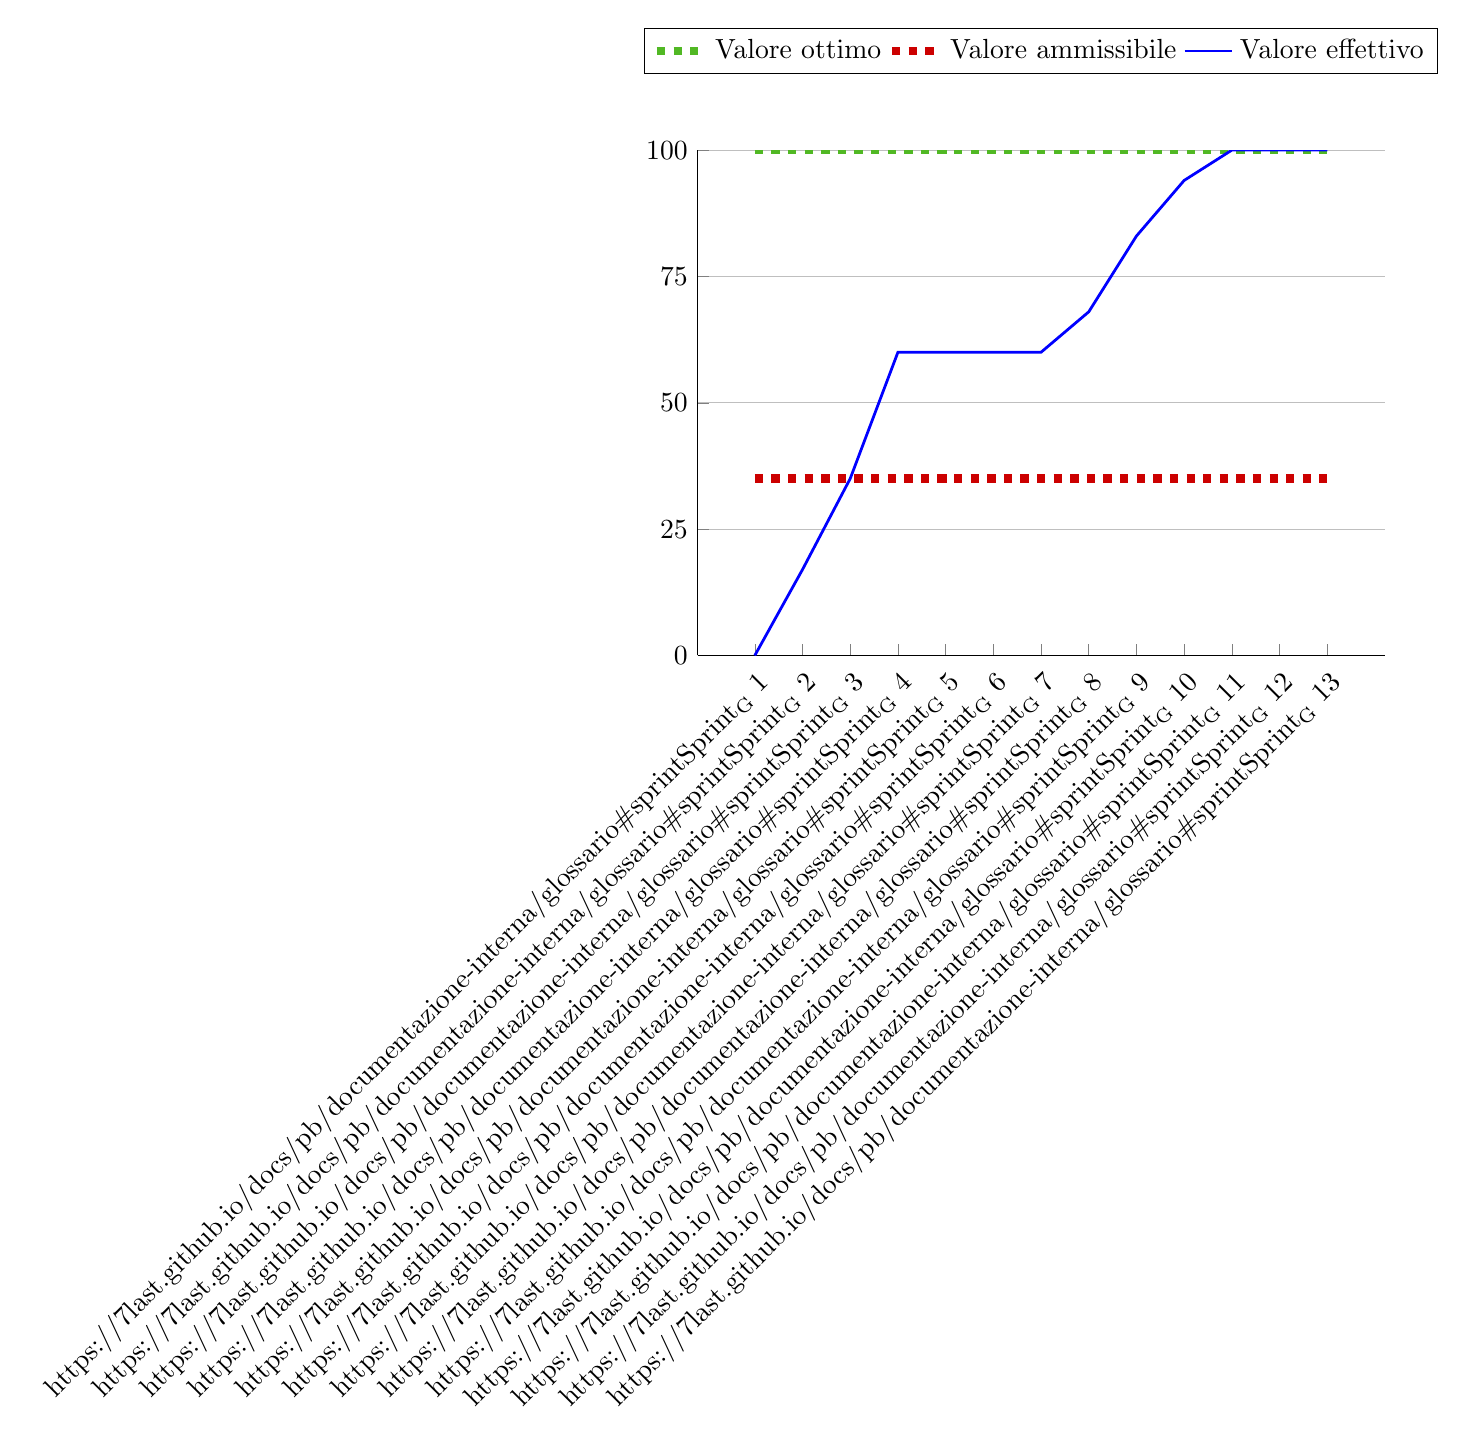
\begin{tikzpicture}
        \begin{axis}[
            width  = 0.85*\textwidth,
            height = 8cm,
            ymajorgrids = true,
            symbolic x coords={\href{https://7last.github.io/docs/pb/documentazione-interna/glossario\#sprint}{Sprint\textsubscript{G}} 1, \href{https://7last.github.io/docs/pb/documentazione-interna/glossario\#sprint}{Sprint\textsubscript{G}} 2, \href{https://7last.github.io/docs/pb/documentazione-interna/glossario\#sprint}{Sprint\textsubscript{G}} 3, \href{https://7last.github.io/docs/pb/documentazione-interna/glossario\#sprint}{Sprint\textsubscript{G}} 4, \href{https://7last.github.io/docs/pb/documentazione-interna/glossario\#sprint}{Sprint\textsubscript{G}} 5, \href{https://7last.github.io/docs/pb/documentazione-interna/glossario\#sprint}{Sprint\textsubscript{G}} 6, \href{https://7last.github.io/docs/pb/documentazione-interna/glossario\#sprint}{Sprint\textsubscript{G}} 7, \href{https://7last.github.io/docs/pb/documentazione-interna/glossario\#sprint}{Sprint\textsubscript{G}} 8, \href{https://7last.github.io/docs/pb/documentazione-interna/glossario\#sprint}{Sprint\textsubscript{G}} 9, \href{https://7last.github.io/docs/pb/documentazione-interna/glossario\#sprint}{Sprint\textsubscript{G}} 10, \href{https://7last.github.io/docs/pb/documentazione-interna/glossario\#sprint}{Sprint\textsubscript{G}} 11, \href{https://7last.github.io/docs/pb/documentazione-interna/glossario\#sprint}{Sprint\textsubscript{G}} 12, \href{https://7last.github.io/docs/pb/documentazione-interna/glossario\#sprint}{Sprint\textsubscript{G}} 13},
            xtick = data,
            ytick = {0, 25, 50, 75, 100},
            ymin=0, ymax=100,
            axis lines*=left,
            legend cell align=left,
            legend style={
                at={(0.5,1.15)},
                anchor=south,
                column sep=0.1ex,
                legend columns=3
            },
            xticklabel style={rotate=45, anchor=north east, yshift=0ex, xshift=0ex}
            ]
            \addplot[color=opt, style={dashed, line width=3pt}, mark=none] coordinates { % ottimo = 100
                (\href{https://7last.github.io/docs/pb/documentazione-interna/glossario\#sprint}{Sprint\textsubscript{G}} 1, 100)
                (\href{https://7last.github.io/docs/pb/documentazione-interna/glossario\#sprint}{Sprint\textsubscript{G}} 2, 100)
                (\href{https://7last.github.io/docs/pb/documentazione-interna/glossario\#sprint}{Sprint\textsubscript{G}} 3, 100)
                (\href{https://7last.github.io/docs/pb/documentazione-interna/glossario\#sprint}{Sprint\textsubscript{G}} 4, 100)
                (\href{https://7last.github.io/docs/pb/documentazione-interna/glossario\#sprint}{Sprint\textsubscript{G}} 5, 100)
                (\href{https://7last.github.io/docs/pb/documentazione-interna/glossario\#sprint}{Sprint\textsubscript{G}} 6, 100)
                (\href{https://7last.github.io/docs/pb/documentazione-interna/glossario\#sprint}{Sprint\textsubscript{G}} 7, 100)
                (\href{https://7last.github.io/docs/pb/documentazione-interna/glossario\#sprint}{Sprint\textsubscript{G}} 8, 100)
                (\href{https://7last.github.io/docs/pb/documentazione-interna/glossario\#sprint}{Sprint\textsubscript{G}} 9, 100)
                (\href{https://7last.github.io/docs/pb/documentazione-interna/glossario\#sprint}{Sprint\textsubscript{G}} 10, 100)
                (\href{https://7last.github.io/docs/pb/documentazione-interna/glossario\#sprint}{Sprint\textsubscript{G}} 11, 100)
                (\href{https://7last.github.io/docs/pb/documentazione-interna/glossario\#sprint}{Sprint\textsubscript{G}} 12, 100)
                (\href{https://7last.github.io/docs/pb/documentazione-interna/glossario\#sprint}{Sprint\textsubscript{G}} 13, 100)
            };
            \addplot[color=amm, style={dashed, line width=3pt}, mark=none] coordinates { % ammissibile = 35
                (\href{https://7last.github.io/docs/pb/documentazione-interna/glossario\#sprint}{Sprint\textsubscript{G}} 1, 35)
                (\href{https://7last.github.io/docs/pb/documentazione-interna/glossario\#sprint}{Sprint\textsubscript{G}} 2, 35)
                (\href{https://7last.github.io/docs/pb/documentazione-interna/glossario\#sprint}{Sprint\textsubscript{G}} 3, 35)
                (\href{https://7last.github.io/docs/pb/documentazione-interna/glossario\#sprint}{Sprint\textsubscript{G}} 4, 35)
                (\href{https://7last.github.io/docs/pb/documentazione-interna/glossario\#sprint}{Sprint\textsubscript{G}} 5, 35)
                (\href{https://7last.github.io/docs/pb/documentazione-interna/glossario\#sprint}{Sprint\textsubscript{G}} 6, 35)
                (\href{https://7last.github.io/docs/pb/documentazione-interna/glossario\#sprint}{Sprint\textsubscript{G}} 7, 35)
                (\href{https://7last.github.io/docs/pb/documentazione-interna/glossario\#sprint}{Sprint\textsubscript{G}} 8, 35)
                (\href{https://7last.github.io/docs/pb/documentazione-interna/glossario\#sprint}{Sprint\textsubscript{G}} 9, 35)
                (\href{https://7last.github.io/docs/pb/documentazione-interna/glossario\#sprint}{Sprint\textsubscript{G}} 10, 35)
                (\href{https://7last.github.io/docs/pb/documentazione-interna/glossario\#sprint}{Sprint\textsubscript{G}} 11, 35)
                (\href{https://7last.github.io/docs/pb/documentazione-interna/glossario\#sprint}{Sprint\textsubscript{G}} 12, 35)
                (\href{https://7last.github.io/docs/pb/documentazione-interna/glossario\#sprint}{Sprint\textsubscript{G}} 13, 35)
            };
            \addplot[color=blue, style={line width=1pt}, mark=none] coordinates { % effettivo
                (\href{https://7last.github.io/docs/pb/documentazione-interna/glossario\#sprint}{Sprint\textsubscript{G}} 1, 0)
                (\href{https://7last.github.io/docs/pb/documentazione-interna/glossario\#sprint}{Sprint\textsubscript{G}} 2, 17)
                (\href{https://7last.github.io/docs/pb/documentazione-interna/glossario\#sprint}{Sprint\textsubscript{G}} 3, 35)
                (\href{https://7last.github.io/docs/pb/documentazione-interna/glossario\#sprint}{Sprint\textsubscript{G}} 4, 60)
                (\href{https://7last.github.io/docs/pb/documentazione-interna/glossario\#sprint}{Sprint\textsubscript{G}} 5, 60)
                (\href{https://7last.github.io/docs/pb/documentazione-interna/glossario\#sprint}{Sprint\textsubscript{G}} 6, 60)
                (\href{https://7last.github.io/docs/pb/documentazione-interna/glossario\#sprint}{Sprint\textsubscript{G}} 7, 60)
                (\href{https://7last.github.io/docs/pb/documentazione-interna/glossario\#sprint}{Sprint\textsubscript{G}} 8, 68)
                (\href{https://7last.github.io/docs/pb/documentazione-interna/glossario\#sprint}{Sprint\textsubscript{G}} 9, 83)
                (\href{https://7last.github.io/docs/pb/documentazione-interna/glossario\#sprint}{Sprint\textsubscript{G}} 10, 94)
                (\href{https://7last.github.io/docs/pb/documentazione-interna/glossario\#sprint}{Sprint\textsubscript{G}} 11, 100)
                (\href{https://7last.github.io/docs/pb/documentazione-interna/glossario\#sprint}{Sprint\textsubscript{G}} 12, 100)
                (\href{https://7last.github.io/docs/pb/documentazione-interna/glossario\#sprint}{Sprint\textsubscript{G}} 13, 100)
            };
            \legend{Valore ottimo, Valore ammissibile, Valore effettivo}
        \end{axis}
    \end{tikzpicture}
    \caption{Percentuale di copertura dei requisiti desiderabili}
\end{figure*}
%--------- FINE GRAFICO -----------% \\
\begin{flushleft}
\href{https://7last.github.io/docs/pb/documentazione-interna/glossario\#product-baseline}{\textbf{PB}\textsubscript{G}} \\
Il grafico mostra come il gruppo \textit{7Last} abbia lavorato per soddisfare i requisiti desiderabili, raggiungendo l'ottimo risultato del 100\% di copertura. Questo conferma che il gruppo ha lavorato in modo efficace e con un'attenzione costante ai requisiti desiderabili.
\end{flushleft}

\newpage
\subsubsection{13M-PRO - Percentuale requisiti opzionali}
%--------- GRAFICO -----------%
\begin{figure*}[!h]
    \centering
    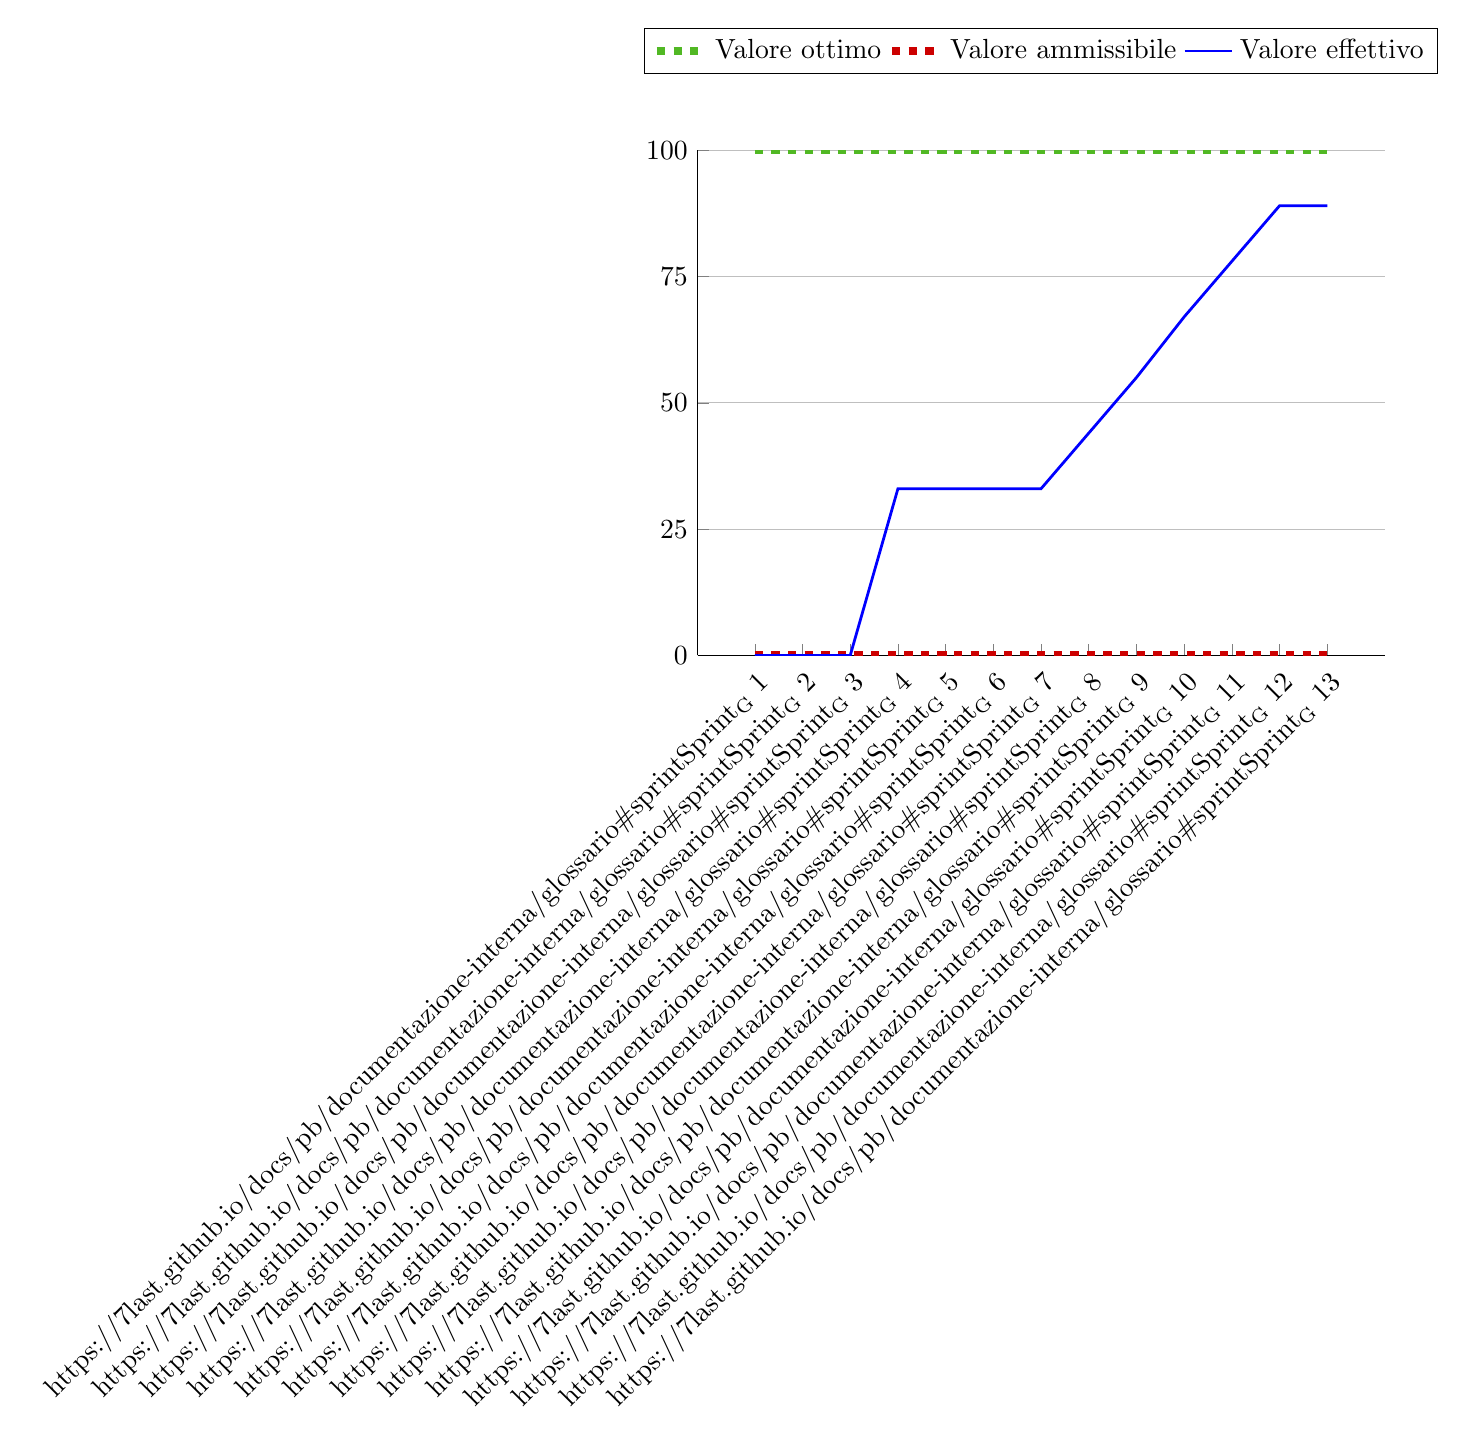
\begin{tikzpicture}
        \begin{axis}[
            width  = 0.85*\textwidth,
            height = 8cm,
            ymajorgrids = true,
            symbolic x coords={\href{https://7last.github.io/docs/pb/documentazione-interna/glossario\#sprint}{Sprint\textsubscript{G}} 1, \href{https://7last.github.io/docs/pb/documentazione-interna/glossario\#sprint}{Sprint\textsubscript{G}} 2, \href{https://7last.github.io/docs/pb/documentazione-interna/glossario\#sprint}{Sprint\textsubscript{G}} 3, \href{https://7last.github.io/docs/pb/documentazione-interna/glossario\#sprint}{Sprint\textsubscript{G}} 4, \href{https://7last.github.io/docs/pb/documentazione-interna/glossario\#sprint}{Sprint\textsubscript{G}} 5, \href{https://7last.github.io/docs/pb/documentazione-interna/glossario\#sprint}{Sprint\textsubscript{G}} 6, \href{https://7last.github.io/docs/pb/documentazione-interna/glossario\#sprint}{Sprint\textsubscript{G}} 7, \href{https://7last.github.io/docs/pb/documentazione-interna/glossario\#sprint}{Sprint\textsubscript{G}} 8, \href{https://7last.github.io/docs/pb/documentazione-interna/glossario\#sprint}{Sprint\textsubscript{G}} 9, \href{https://7last.github.io/docs/pb/documentazione-interna/glossario\#sprint}{Sprint\textsubscript{G}} 10, \href{https://7last.github.io/docs/pb/documentazione-interna/glossario\#sprint}{Sprint\textsubscript{G}} 11, \href{https://7last.github.io/docs/pb/documentazione-interna/glossario\#sprint}{Sprint\textsubscript{G}} 12, \href{https://7last.github.io/docs/pb/documentazione-interna/glossario\#sprint}{Sprint\textsubscript{G}} 13},
            xtick = data,
            ytick = {0, 25, 50, 75, 100},
            ymin=0, ymax=100,
            axis lines*=left,
            legend cell align=left,
            legend style={
                at={(0.5,1.15)},
                anchor=south,
                column sep=0.1ex,
                legend columns=3
            },
            xticklabel style={rotate=45, anchor=north east, yshift=0ex, xshift=0ex}
            ]
            \addplot[color=opt, style={dashed, line width=3pt}, mark=none] coordinates { % ottimo = 100
                (\href{https://7last.github.io/docs/pb/documentazione-interna/glossario\#sprint}{Sprint\textsubscript{G}} 1, 100)
                (\href{https://7last.github.io/docs/pb/documentazione-interna/glossario\#sprint}{Sprint\textsubscript{G}} 2, 100)
                (\href{https://7last.github.io/docs/pb/documentazione-interna/glossario\#sprint}{Sprint\textsubscript{G}} 3, 100)
                (\href{https://7last.github.io/docs/pb/documentazione-interna/glossario\#sprint}{Sprint\textsubscript{G}} 4, 100)
                (\href{https://7last.github.io/docs/pb/documentazione-interna/glossario\#sprint}{Sprint\textsubscript{G}} 5, 100)
                (\href{https://7last.github.io/docs/pb/documentazione-interna/glossario\#sprint}{Sprint\textsubscript{G}} 6, 100)
                (\href{https://7last.github.io/docs/pb/documentazione-interna/glossario\#sprint}{Sprint\textsubscript{G}} 7, 100)
                (\href{https://7last.github.io/docs/pb/documentazione-interna/glossario\#sprint}{Sprint\textsubscript{G}} 8, 100)
                (\href{https://7last.github.io/docs/pb/documentazione-interna/glossario\#sprint}{Sprint\textsubscript{G}} 9, 100)
                (\href{https://7last.github.io/docs/pb/documentazione-interna/glossario\#sprint}{Sprint\textsubscript{G}} 10, 100)
                (\href{https://7last.github.io/docs/pb/documentazione-interna/glossario\#sprint}{Sprint\textsubscript{G}} 11, 100)
                (\href{https://7last.github.io/docs/pb/documentazione-interna/glossario\#sprint}{Sprint\textsubscript{G}} 12, 100)
                (\href{https://7last.github.io/docs/pb/documentazione-interna/glossario\#sprint}{Sprint\textsubscript{G}} 13, 100)
            };
            \addplot[color=amm, style={dashed, line width=3pt}, mark=none] coordinates { % ammissibile = 0
                (\href{https://7last.github.io/docs/pb/documentazione-interna/glossario\#sprint}{Sprint\textsubscript{G}} 1, 0)
                (\href{https://7last.github.io/docs/pb/documentazione-interna/glossario\#sprint}{Sprint\textsubscript{G}} 2, 0)
                (\href{https://7last.github.io/docs/pb/documentazione-interna/glossario\#sprint}{Sprint\textsubscript{G}} 3, 0)
                (\href{https://7last.github.io/docs/pb/documentazione-interna/glossario\#sprint}{Sprint\textsubscript{G}} 4, 0)
                (\href{https://7last.github.io/docs/pb/documentazione-interna/glossario\#sprint}{Sprint\textsubscript{G}} 5, 0)
                (\href{https://7last.github.io/docs/pb/documentazione-interna/glossario\#sprint}{Sprint\textsubscript{G}} 6, 0)
                (\href{https://7last.github.io/docs/pb/documentazione-interna/glossario\#sprint}{Sprint\textsubscript{G}} 7, 0)
                (\href{https://7last.github.io/docs/pb/documentazione-interna/glossario\#sprint}{Sprint\textsubscript{G}} 8, 0)
                (\href{https://7last.github.io/docs/pb/documentazione-interna/glossario\#sprint}{Sprint\textsubscript{G}} 9, 0)
                (\href{https://7last.github.io/docs/pb/documentazione-interna/glossario\#sprint}{Sprint\textsubscript{G}} 10, 0)
                (\href{https://7last.github.io/docs/pb/documentazione-interna/glossario\#sprint}{Sprint\textsubscript{G}} 11, 0)
                (\href{https://7last.github.io/docs/pb/documentazione-interna/glossario\#sprint}{Sprint\textsubscript{G}} 12, 0)
                (\href{https://7last.github.io/docs/pb/documentazione-interna/glossario\#sprint}{Sprint\textsubscript{G}} 13, 0)
            };
            \addplot[color=blue, style={line width=1pt}, mark=none] coordinates { % effettivo
                (\href{https://7last.github.io/docs/pb/documentazione-interna/glossario\#sprint}{Sprint\textsubscript{G}} 1, 0)
                (\href{https://7last.github.io/docs/pb/documentazione-interna/glossario\#sprint}{Sprint\textsubscript{G}} 2, 0)
                (\href{https://7last.github.io/docs/pb/documentazione-interna/glossario\#sprint}{Sprint\textsubscript{G}} 3, 0)
                (\href{https://7last.github.io/docs/pb/documentazione-interna/glossario\#sprint}{Sprint\textsubscript{G}} 4, 33)
                (\href{https://7last.github.io/docs/pb/documentazione-interna/glossario\#sprint}{Sprint\textsubscript{G}} 5, 33)
                (\href{https://7last.github.io/docs/pb/documentazione-interna/glossario\#sprint}{Sprint\textsubscript{G}} 6, 33)
                (\href{https://7last.github.io/docs/pb/documentazione-interna/glossario\#sprint}{Sprint\textsubscript{G}} 7, 33)
                (\href{https://7last.github.io/docs/pb/documentazione-interna/glossario\#sprint}{Sprint\textsubscript{G}} 8, 44)
                (\href{https://7last.github.io/docs/pb/documentazione-interna/glossario\#sprint}{Sprint\textsubscript{G}} 9, 55)
                (\href{https://7last.github.io/docs/pb/documentazione-interna/glossario\#sprint}{Sprint\textsubscript{G}} 10, 67)
                (\href{https://7last.github.io/docs/pb/documentazione-interna/glossario\#sprint}{Sprint\textsubscript{G}} 11, 78)
                (\href{https://7last.github.io/docs/pb/documentazione-interna/glossario\#sprint}{Sprint\textsubscript{G}} 12, 89)
                (\href{https://7last.github.io/docs/pb/documentazione-interna/glossario\#sprint}{Sprint\textsubscript{G}} 13, 89)
            };
            \legend{Valore ottimo, Valore ammissibile, Valore effettivo}
        \end{axis}
    \end{tikzpicture}
    \caption{Percentuale di copertura dei requisiti opzionali}
\end{figure*}
%--------- FINE GRAFICO -----------% \\
\begin{flushleft}
\href{https://7last.github.io/docs/pb/documentazione-interna/glossario\#product-baseline}{\textbf{PB}\textsubscript{G}} \\
Il grafico mostra come il gruppo \textit{7Last} abbia lavorato per soddisfare i requisiti opzionali, con una crescita quasi costante della percentuale di requisiti soddisfatti. Questo conferma che il gruppo ha lavorato in modo efficace. 
\end{flushleft}

\newpage
\subsection{Qualità del processo di documentazione}
\subsubsection{19M-IG - Indice di Gulpease}
%--------- GRAFICO -----------%
\begin{figure*}[!h]
    \centering
    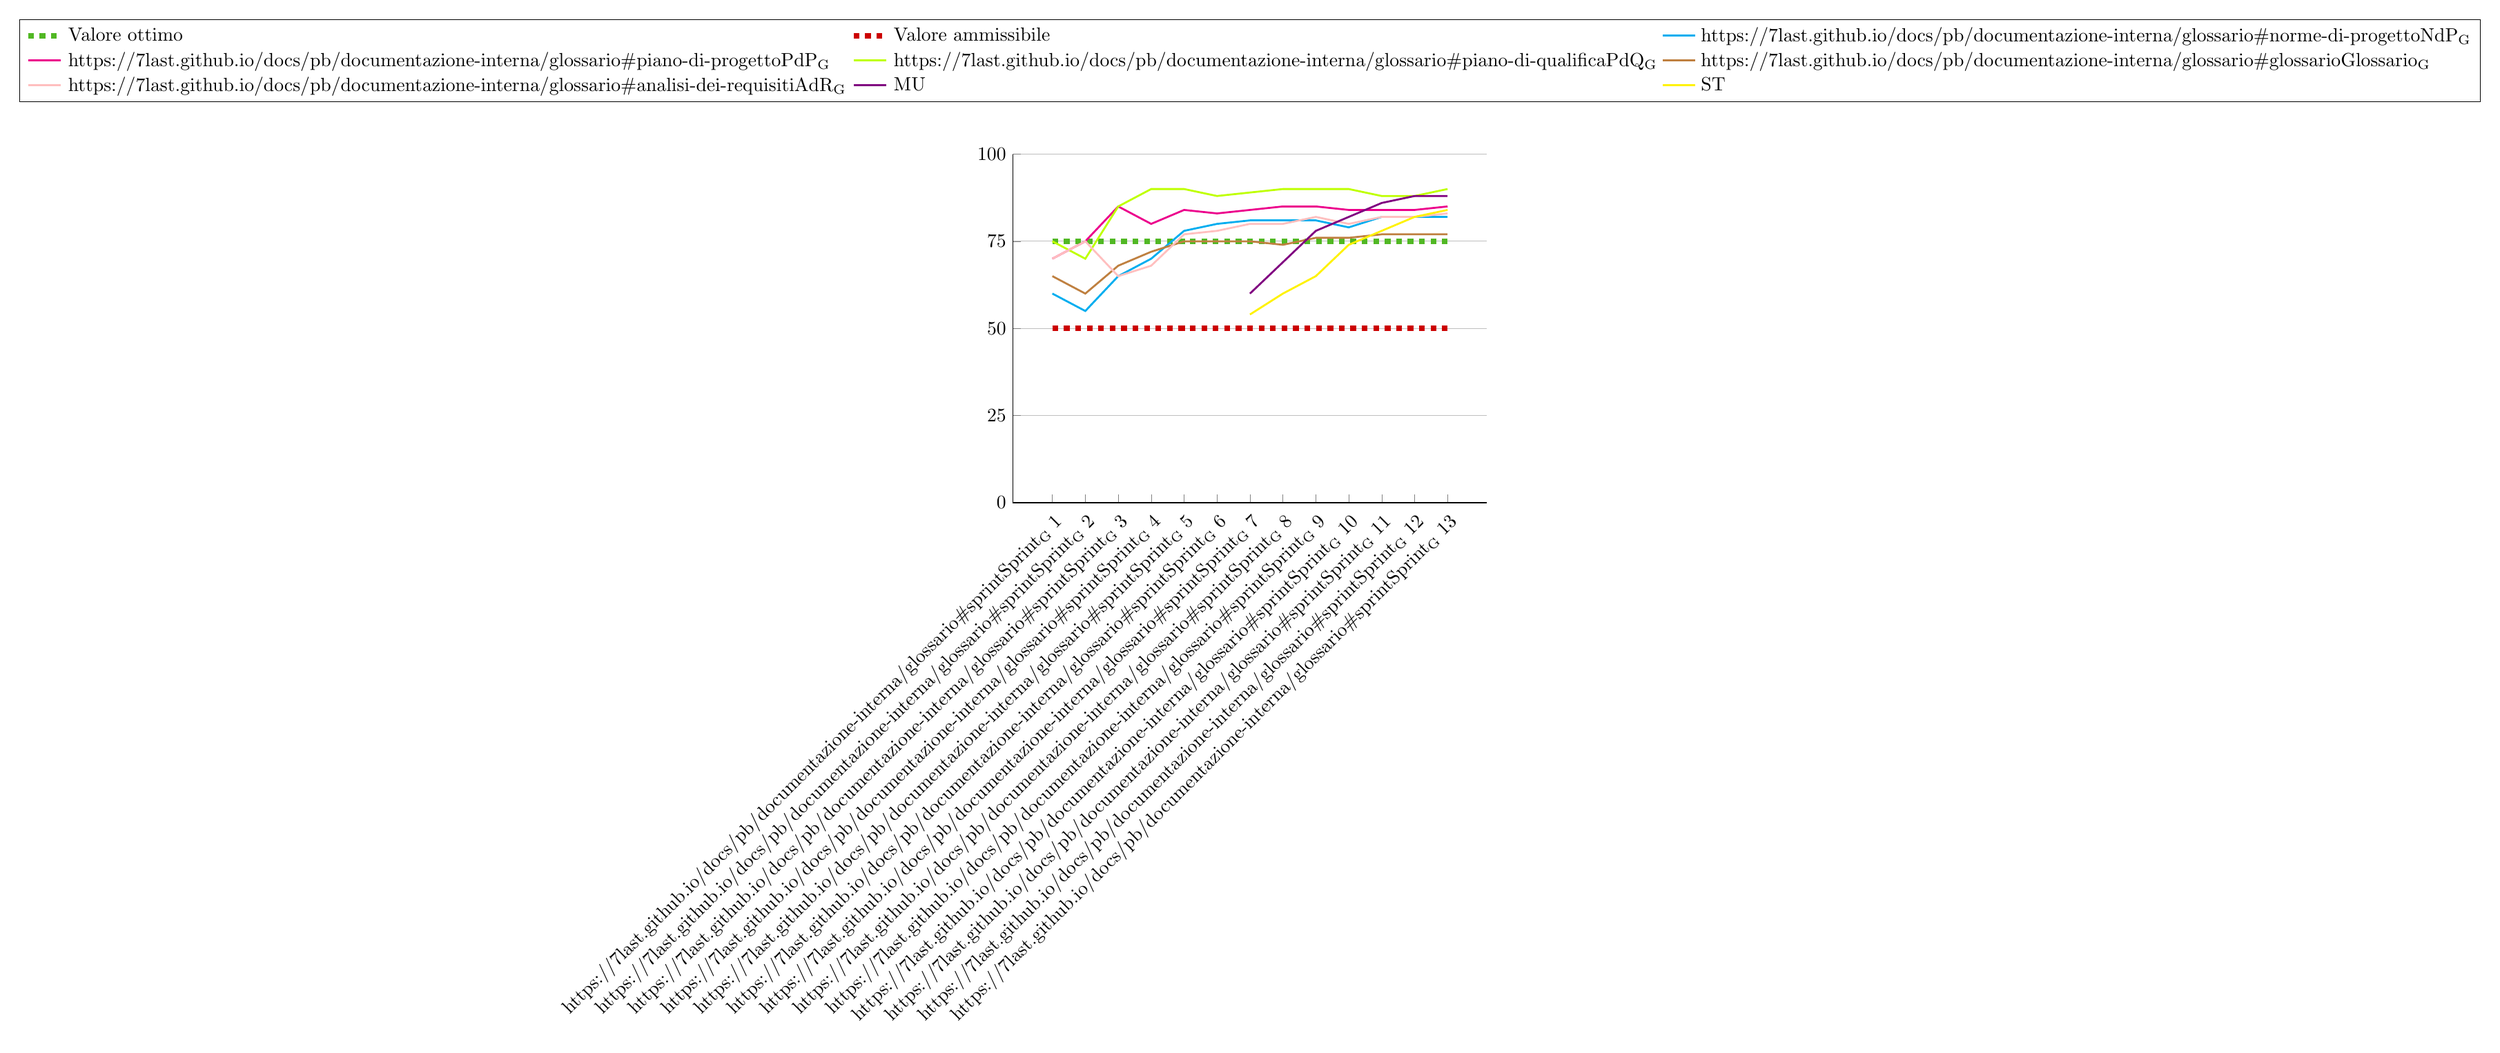
\begin{tikzpicture}
        \begin{axis}[
            width  = 0.85*\textwidth,
            height = 8cm,
            ymajorgrids = true,
            symbolic x coords={\href{https://7last.github.io/docs/pb/documentazione-interna/glossario\#sprint}{Sprint\textsubscript{G}} 1, \href{https://7last.github.io/docs/pb/documentazione-interna/glossario\#sprint}{Sprint\textsubscript{G}} 2, \href{https://7last.github.io/docs/pb/documentazione-interna/glossario\#sprint}{Sprint\textsubscript{G}} 3, \href{https://7last.github.io/docs/pb/documentazione-interna/glossario\#sprint}{Sprint\textsubscript{G}} 4, \href{https://7last.github.io/docs/pb/documentazione-interna/glossario\#sprint}{Sprint\textsubscript{G}} 5, \href{https://7last.github.io/docs/pb/documentazione-interna/glossario\#sprint}{Sprint\textsubscript{G}} 6, \href{https://7last.github.io/docs/pb/documentazione-interna/glossario\#sprint}{Sprint\textsubscript{G}} 7, \href{https://7last.github.io/docs/pb/documentazione-interna/glossario\#sprint}{Sprint\textsubscript{G}} 8, \href{https://7last.github.io/docs/pb/documentazione-interna/glossario\#sprint}{Sprint\textsubscript{G}} 9, \href{https://7last.github.io/docs/pb/documentazione-interna/glossario\#sprint}{Sprint\textsubscript{G}} 10, \href{https://7last.github.io/docs/pb/documentazione-interna/glossario\#sprint}{Sprint\textsubscript{G}} 11, \href{https://7last.github.io/docs/pb/documentazione-interna/glossario\#sprint}{Sprint\textsubscript{G}} 12, \href{https://7last.github.io/docs/pb/documentazione-interna/glossario\#sprint}{Sprint\textsubscript{G}} 13},
            xtick = data,
            ytick = {0, 25, 50, 75, 100},
            ymin=0, ymax=100,
            axis lines*=left,
            legend cell align=left,
            legend style={
                at={(0.5,1.15)},
                anchor=south,
                column sep=0.1ex,
                legend columns=3
            },
            xticklabel style={rotate=45, anchor=north east, yshift=0ex, xshift=0ex}
        ]
            \addplot[color=opt, style={dashed, line width=3pt}, mark=none] coordinates { % ottimo = 75
                (\href{https://7last.github.io/docs/pb/documentazione-interna/glossario\#sprint}{Sprint\textsubscript{G}} 1, 75)
                (\href{https://7last.github.io/docs/pb/documentazione-interna/glossario\#sprint}{Sprint\textsubscript{G}} 2, 75)
                (\href{https://7last.github.io/docs/pb/documentazione-interna/glossario\#sprint}{Sprint\textsubscript{G}} 3, 75)
                (\href{https://7last.github.io/docs/pb/documentazione-interna/glossario\#sprint}{Sprint\textsubscript{G}} 4, 75)
                (\href{https://7last.github.io/docs/pb/documentazione-interna/glossario\#sprint}{Sprint\textsubscript{G}} 5, 75)
                (\href{https://7last.github.io/docs/pb/documentazione-interna/glossario\#sprint}{Sprint\textsubscript{G}} 6, 75)
                (\href{https://7last.github.io/docs/pb/documentazione-interna/glossario\#sprint}{Sprint\textsubscript{G}} 7, 75)
                (\href{https://7last.github.io/docs/pb/documentazione-interna/glossario\#sprint}{Sprint\textsubscript{G}} 8, 75)
                (\href{https://7last.github.io/docs/pb/documentazione-interna/glossario\#sprint}{Sprint\textsubscript{G}} 9, 75)
                (\href{https://7last.github.io/docs/pb/documentazione-interna/glossario\#sprint}{Sprint\textsubscript{G}} 10, 75)
                (\href{https://7last.github.io/docs/pb/documentazione-interna/glossario\#sprint}{Sprint\textsubscript{G}} 11, 75)
                (\href{https://7last.github.io/docs/pb/documentazione-interna/glossario\#sprint}{Sprint\textsubscript{G}} 12, 75)
                (\href{https://7last.github.io/docs/pb/documentazione-interna/glossario\#sprint}{Sprint\textsubscript{G}} 13, 75)
            };
            \addplot[color=amm, style={dashed, line width=3pt}, mark=none] coordinates { % ammissibile = 50
                (\href{https://7last.github.io/docs/pb/documentazione-interna/glossario\#sprint}{Sprint\textsubscript{G}} 1, 50)
                (\href{https://7last.github.io/docs/pb/documentazione-interna/glossario\#sprint}{Sprint\textsubscript{G}} 2, 50)
                (\href{https://7last.github.io/docs/pb/documentazione-interna/glossario\#sprint}{Sprint\textsubscript{G}} 3, 50)
                (\href{https://7last.github.io/docs/pb/documentazione-interna/glossario\#sprint}{Sprint\textsubscript{G}} 4, 50)
                (\href{https://7last.github.io/docs/pb/documentazione-interna/glossario\#sprint}{Sprint\textsubscript{G}} 5, 50)
                (\href{https://7last.github.io/docs/pb/documentazione-interna/glossario\#sprint}{Sprint\textsubscript{G}} 6, 50)
                (\href{https://7last.github.io/docs/pb/documentazione-interna/glossario\#sprint}{Sprint\textsubscript{G}} 7, 50)
                (\href{https://7last.github.io/docs/pb/documentazione-interna/glossario\#sprint}{Sprint\textsubscript{G}} 8, 50)
                (\href{https://7last.github.io/docs/pb/documentazione-interna/glossario\#sprint}{Sprint\textsubscript{G}} 9, 50)
                (\href{https://7last.github.io/docs/pb/documentazione-interna/glossario\#sprint}{Sprint\textsubscript{G}} 10, 50)
                (\href{https://7last.github.io/docs/pb/documentazione-interna/glossario\#sprint}{Sprint\textsubscript{G}} 11, 50)
                (\href{https://7last.github.io/docs/pb/documentazione-interna/glossario\#sprint}{Sprint\textsubscript{G}} 12, 50)
                (\href{https://7last.github.io/docs/pb/documentazione-interna/glossario\#sprint}{Sprint\textsubscript{G}} 13, 50)
            };
            \addplot[color=cyan, style={line width=1pt}, mark=none] coordinates { % \href{https://7last.github.io/docs/pb/documentazione-interna/glossario\#norme-di-progetto}{norme di progetto\textsubscript{G}}
                (\href{https://7last.github.io/docs/pb/documentazione-interna/glossario\#sprint}{Sprint\textsubscript{G}} 1, 60)
                (\href{https://7last.github.io/docs/pb/documentazione-interna/glossario\#sprint}{Sprint\textsubscript{G}} 2, 55)
                (\href{https://7last.github.io/docs/pb/documentazione-interna/glossario\#sprint}{Sprint\textsubscript{G}} 3, 65)
                (\href{https://7last.github.io/docs/pb/documentazione-interna/glossario\#sprint}{Sprint\textsubscript{G}} 4, 70)
                (\href{https://7last.github.io/docs/pb/documentazione-interna/glossario\#sprint}{Sprint\textsubscript{G}} 5, 78)
                (\href{https://7last.github.io/docs/pb/documentazione-interna/glossario\#sprint}{Sprint\textsubscript{G}} 6, 80)
                (\href{https://7last.github.io/docs/pb/documentazione-interna/glossario\#sprint}{Sprint\textsubscript{G}} 7, 81)
                (\href{https://7last.github.io/docs/pb/documentazione-interna/glossario\#sprint}{Sprint\textsubscript{G}} 8, 81)
                (\href{https://7last.github.io/docs/pb/documentazione-interna/glossario\#sprint}{Sprint\textsubscript{G}} 9, 81)
                (\href{https://7last.github.io/docs/pb/documentazione-interna/glossario\#sprint}{Sprint\textsubscript{G}} 10, 79)
                (\href{https://7last.github.io/docs/pb/documentazione-interna/glossario\#sprint}{Sprint\textsubscript{G}} 11, 82)
                (\href{https://7last.github.io/docs/pb/documentazione-interna/glossario\#sprint}{Sprint\textsubscript{G}} 12, 82)
                (\href{https://7last.github.io/docs/pb/documentazione-interna/glossario\#sprint}{Sprint\textsubscript{G}} 13, 82)
            };
            \addplot[color=magenta, style={line width=1pt}, mark=none] coordinates { % \href{https://7last.github.io/docs/pb/documentazione-interna/glossario\#piano-di-progetto}{piano di progetto\textsubscript{G}}
                (\href{https://7last.github.io/docs/pb/documentazione-interna/glossario\#sprint}{Sprint\textsubscript{G}} 1, 70)
                (\href{https://7last.github.io/docs/pb/documentazione-interna/glossario\#sprint}{Sprint\textsubscript{G}} 2, 75)
                (\href{https://7last.github.io/docs/pb/documentazione-interna/glossario\#sprint}{Sprint\textsubscript{G}} 3, 85)
                (\href{https://7last.github.io/docs/pb/documentazione-interna/glossario\#sprint}{Sprint\textsubscript{G}} 4, 80)
                (\href{https://7last.github.io/docs/pb/documentazione-interna/glossario\#sprint}{Sprint\textsubscript{G}} 5, 84)
                (\href{https://7last.github.io/docs/pb/documentazione-interna/glossario\#sprint}{Sprint\textsubscript{G}} 6, 83)
                (\href{https://7last.github.io/docs/pb/documentazione-interna/glossario\#sprint}{Sprint\textsubscript{G}} 7, 84)
                (\href{https://7last.github.io/docs/pb/documentazione-interna/glossario\#sprint}{Sprint\textsubscript{G}} 8, 85)
                (\href{https://7last.github.io/docs/pb/documentazione-interna/glossario\#sprint}{Sprint\textsubscript{G}} 9, 85)
                (\href{https://7last.github.io/docs/pb/documentazione-interna/glossario\#sprint}{Sprint\textsubscript{G}} 10, 84)
                (\href{https://7last.github.io/docs/pb/documentazione-interna/glossario\#sprint}{Sprint\textsubscript{G}} 11, 84)
                (\href{https://7last.github.io/docs/pb/documentazione-interna/glossario\#sprint}{Sprint\textsubscript{G}} 12, 84)
                (\href{https://7last.github.io/docs/pb/documentazione-interna/glossario\#sprint}{Sprint\textsubscript{G}} 13, 85)
            };
            \addplot[color=lime, style={line width=1pt}, mark=none] coordinates { % \href{https://7last.github.io/docs/pb/documentazione-interna/glossario\#piano-di-qualifica}{piano di qualifica\textsubscript{G}}
                (\href{https://7last.github.io/docs/pb/documentazione-interna/glossario\#sprint}{Sprint\textsubscript{G}} 1, 75)
                (\href{https://7last.github.io/docs/pb/documentazione-interna/glossario\#sprint}{Sprint\textsubscript{G}} 2, 70)
                (\href{https://7last.github.io/docs/pb/documentazione-interna/glossario\#sprint}{Sprint\textsubscript{G}} 3, 85)
                (\href{https://7last.github.io/docs/pb/documentazione-interna/glossario\#sprint}{Sprint\textsubscript{G}} 4, 90)
                (\href{https://7last.github.io/docs/pb/documentazione-interna/glossario\#sprint}{Sprint\textsubscript{G}} 5, 90)
                (\href{https://7last.github.io/docs/pb/documentazione-interna/glossario\#sprint}{Sprint\textsubscript{G}} 6, 88)
                (\href{https://7last.github.io/docs/pb/documentazione-interna/glossario\#sprint}{Sprint\textsubscript{G}} 7, 89)
                (\href{https://7last.github.io/docs/pb/documentazione-interna/glossario\#sprint}{Sprint\textsubscript{G}} 8, 90)
                (\href{https://7last.github.io/docs/pb/documentazione-interna/glossario\#sprint}{Sprint\textsubscript{G}} 9, 90)
                (\href{https://7last.github.io/docs/pb/documentazione-interna/glossario\#sprint}{Sprint\textsubscript{G}} 10, 90)
                (\href{https://7last.github.io/docs/pb/documentazione-interna/glossario\#sprint}{Sprint\textsubscript{G}} 11, 88)
                (\href{https://7last.github.io/docs/pb/documentazione-interna/glossario\#sprint}{Sprint\textsubscript{G}} 12, 88)
                (\href{https://7last.github.io/docs/pb/documentazione-interna/glossario\#sprint}{Sprint\textsubscript{G}} 13, 90)
            };
            \addplot[color=brown, style={line width=1pt}, mark=none] coordinates { % \href{https://7last.github.io/docs/pb/documentazione-interna/glossario\#glossario}{glossario\textsubscript{G}}
                (\href{https://7last.github.io/docs/pb/documentazione-interna/glossario\#sprint}{Sprint\textsubscript{G}} 1, 65)
                (\href{https://7last.github.io/docs/pb/documentazione-interna/glossario\#sprint}{Sprint\textsubscript{G}} 2, 60)
                (\href{https://7last.github.io/docs/pb/documentazione-interna/glossario\#sprint}{Sprint\textsubscript{G}} 3, 68)
                (\href{https://7last.github.io/docs/pb/documentazione-interna/glossario\#sprint}{Sprint\textsubscript{G}} 4, 72)
                (\href{https://7last.github.io/docs/pb/documentazione-interna/glossario\#sprint}{Sprint\textsubscript{G}} 5, 75)
                (\href{https://7last.github.io/docs/pb/documentazione-interna/glossario\#sprint}{Sprint\textsubscript{G}} 6, 75)
                (\href{https://7last.github.io/docs/pb/documentazione-interna/glossario\#sprint}{Sprint\textsubscript{G}} 7, 75)
                (\href{https://7last.github.io/docs/pb/documentazione-interna/glossario\#sprint}{Sprint\textsubscript{G}} 8, 74)
                (\href{https://7last.github.io/docs/pb/documentazione-interna/glossario\#sprint}{Sprint\textsubscript{G}} 9, 76)
                (\href{https://7last.github.io/docs/pb/documentazione-interna/glossario\#sprint}{Sprint\textsubscript{G}} 10, 76)
                (\href{https://7last.github.io/docs/pb/documentazione-interna/glossario\#sprint}{Sprint\textsubscript{G}} 11, 77)
                (\href{https://7last.github.io/docs/pb/documentazione-interna/glossario\#sprint}{Sprint\textsubscript{G}} 12, 77)
                (\href{https://7last.github.io/docs/pb/documentazione-interna/glossario\#sprint}{Sprint\textsubscript{G}} 13, 77)
            };
            \addplot[color=pink, style={line width=1pt}, mark=none] coordinates { % \href{https://7last.github.io/docs/pb/documentazione-interna/glossario\#analisi-dei-requisiti}{analisi dei requisiti\textsubscript{G}}
                (\href{https://7last.github.io/docs/pb/documentazione-interna/glossario\#sprint}{Sprint\textsubscript{G}} 1, 70)
                (\href{https://7last.github.io/docs/pb/documentazione-interna/glossario\#sprint}{Sprint\textsubscript{G}} 2, 75)
                (\href{https://7last.github.io/docs/pb/documentazione-interna/glossario\#sprint}{Sprint\textsubscript{G}} 3, 65)
                (\href{https://7last.github.io/docs/pb/documentazione-interna/glossario\#sprint}{Sprint\textsubscript{G}} 4, 68)
                (\href{https://7last.github.io/docs/pb/documentazione-interna/glossario\#sprint}{Sprint\textsubscript{G}} 5, 77)
                (\href{https://7last.github.io/docs/pb/documentazione-interna/glossario\#sprint}{Sprint\textsubscript{G}} 6, 78)
                (\href{https://7last.github.io/docs/pb/documentazione-interna/glossario\#sprint}{Sprint\textsubscript{G}} 7, 80)
                (\href{https://7last.github.io/docs/pb/documentazione-interna/glossario\#sprint}{Sprint\textsubscript{G}} 8, 80)
                (\href{https://7last.github.io/docs/pb/documentazione-interna/glossario\#sprint}{Sprint\textsubscript{G}} 9, 82)
                (\href{https://7last.github.io/docs/pb/documentazione-interna/glossario\#sprint}{Sprint\textsubscript{G}} 10, 80)
                (\href{https://7last.github.io/docs/pb/documentazione-interna/glossario\#sprint}{Sprint\textsubscript{G}} 11, 82)
                (\href{https://7last.github.io/docs/pb/documentazione-interna/glossario\#sprint}{Sprint\textsubscript{G}} 12, 82)
                (\href{https://7last.github.io/docs/pb/documentazione-interna/glossario\#sprint}{Sprint\textsubscript{G}} 13, 83)
            };
            \addplot[color=violet, style={line width=1pt}, mark=none] coordinates { % manuale utente
                (\href{https://7last.github.io/docs/pb/documentazione-interna/glossario\#sprint}{Sprint\textsubscript{G}} 7, 60)
                (\href{https://7last.github.io/docs/pb/documentazione-interna/glossario\#sprint}{Sprint\textsubscript{G}} 8, 69)
                (\href{https://7last.github.io/docs/pb/documentazione-interna/glossario\#sprint}{Sprint\textsubscript{G}} 9, 78)
                (\href{https://7last.github.io/docs/pb/documentazione-interna/glossario\#sprint}{Sprint\textsubscript{G}} 10, 82)
                (\href{https://7last.github.io/docs/pb/documentazione-interna/glossario\#sprint}{Sprint\textsubscript{G}} 11, 86)
                (\href{https://7last.github.io/docs/pb/documentazione-interna/glossario\#sprint}{Sprint\textsubscript{G}} 12, 88)
                (\href{https://7last.github.io/docs/pb/documentazione-interna/glossario\#sprint}{Sprint\textsubscript{G}} 13, 88)
            };
            \addplot[color=yellow, style={line width=1pt}, mark=none] coordinates { % specifica tecnica
                (\href{https://7last.github.io/docs/pb/documentazione-interna/glossario\#sprint}{Sprint\textsubscript{G}} 7, 54)
                (\href{https://7last.github.io/docs/pb/documentazione-interna/glossario\#sprint}{Sprint\textsubscript{G}} 8, 60)
                (\href{https://7last.github.io/docs/pb/documentazione-interna/glossario\#sprint}{Sprint\textsubscript{G}} 9, 65)
                (\href{https://7last.github.io/docs/pb/documentazione-interna/glossario\#sprint}{Sprint\textsubscript{G}} 10, 74)
                (\href{https://7last.github.io/docs/pb/documentazione-interna/glossario\#sprint}{Sprint\textsubscript{G}} 11, 78)
                (\href{https://7last.github.io/docs/pb/documentazione-interna/glossario\#sprint}{Sprint\textsubscript{G}} 12, 82)
                (\href{https://7last.github.io/docs/pb/documentazione-interna/glossario\#sprint}{Sprint\textsubscript{G}} 13, 84)
            };
            \legend{Valore ottimo, Valore ammissibile, \href{https://7last.github.io/docs/pb/documentazione-interna/glossario\#norme-di-progetto}{NdP\textsubscript{G}}, \href{https://7last.github.io/docs/pb/documentazione-interna/glossario\#piano-di-progetto}{PdP\textsubscript{G}}, \href{https://7last.github.io/docs/pb/documentazione-interna/glossario\#piano-di-qualifica}{PdQ\textsubscript{G}}, \href{https://7last.github.io/docs/pb/documentazione-interna/glossario\#glossario}{Glossario\textsubscript{G}}, \href{https://7last.github.io/docs/pb/documentazione-interna/glossario\#analisi-dei-requisiti}{AdR\textsubscript{G}}, MU, ST}
        \end{axis}
    \end{tikzpicture}
    \caption{Andamento indice di Gulpease per ciascun documento}
\end{figure*}
%--------- FINE GRAFICO -----------%
\begin{flushleft}
\href{https://7last.github.io/docs/pb/documentazione-interna/glossario\#requirements-and-technology-baseline}{\textbf{RTB}\textsubscript{G}} \\
Visionando il grafico si può notare una tendenza generale di crescita, eccetto per alcuni documenti. L'indice relativamente basso rispetto agli altri documenti rappresenta il \href{https://7last.github.io/docs/pb/documentazione-interna/glossario\#glossario}{glossario\textsubscript{G}}, il quale contiene descrizioni di natura tecnica che possono influire negativamente sull'indice di Gulpease. \\
\href{https://7last.github.io/docs/pb/documentazione-interna/glossario\#product-baseline}{\textbf{PB}\textsubscript{G}} \\
Il grafico mostra come la qualità della documentazione prodotta verso la fine del progetto sia sempre sopra il valore ottimo prestabilito, con un andamento generale di crescita. 
\end{flushleft}

\newpage
\subsubsection{20M-CO - Correttezza ortografica}
%--------- GRAFICO -----------%
\begin{figure*}[!h]
    \centering
    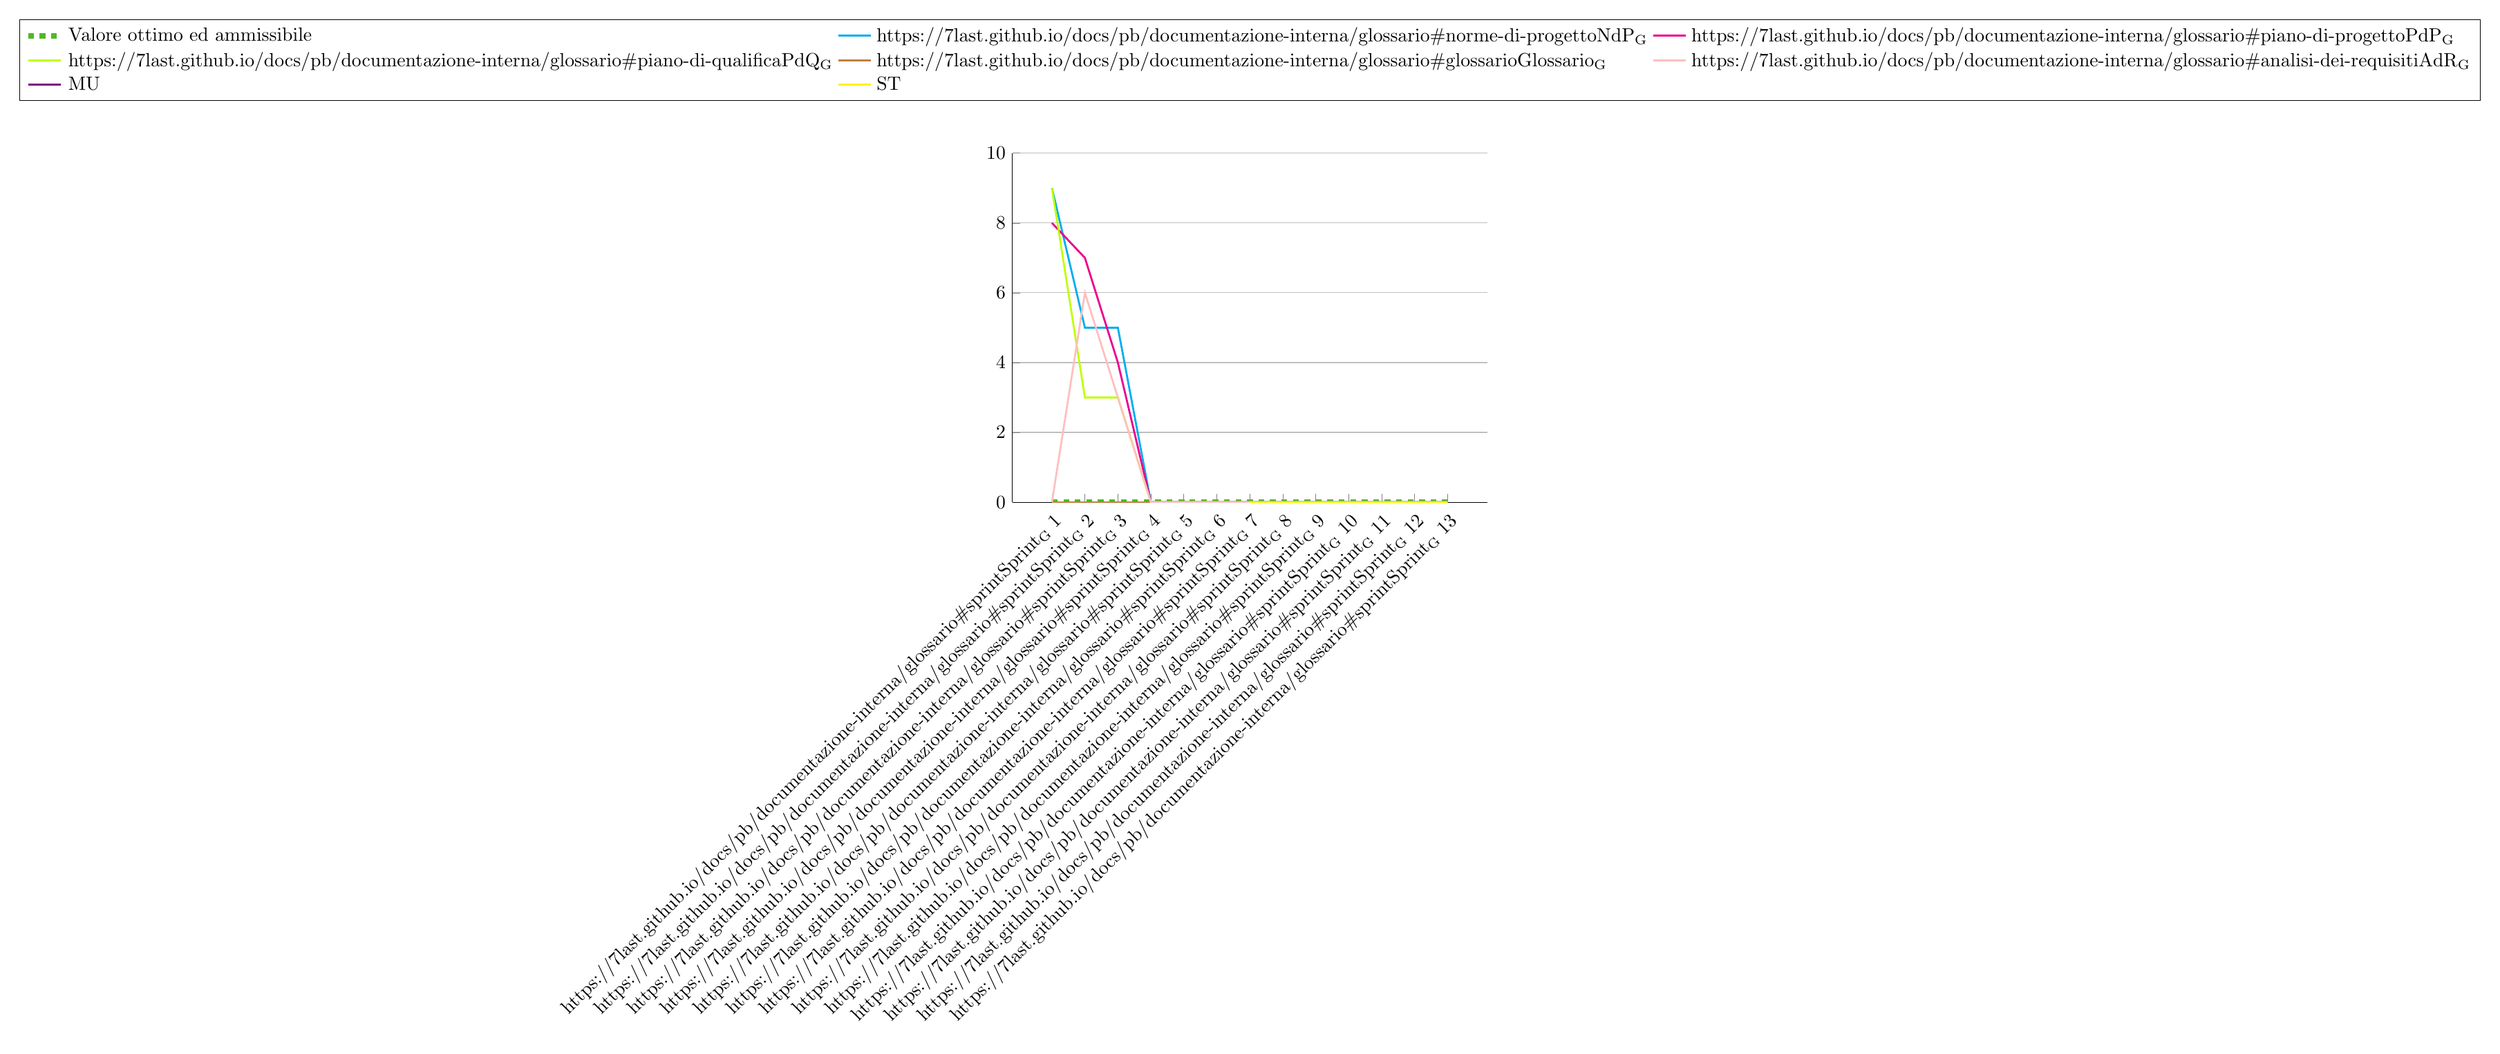
\begin{tikzpicture}
        \begin{axis}[
            width  = 0.85*\textwidth,
            height = 8cm,
            ymajorgrids = true,
            symbolic x coords={\href{https://7last.github.io/docs/pb/documentazione-interna/glossario\#sprint}{Sprint\textsubscript{G}} 1, \href{https://7last.github.io/docs/pb/documentazione-interna/glossario\#sprint}{Sprint\textsubscript{G}} 2, \href{https://7last.github.io/docs/pb/documentazione-interna/glossario\#sprint}{Sprint\textsubscript{G}} 3, \href{https://7last.github.io/docs/pb/documentazione-interna/glossario\#sprint}{Sprint\textsubscript{G}} 4, \href{https://7last.github.io/docs/pb/documentazione-interna/glossario\#sprint}{Sprint\textsubscript{G}} 5, \href{https://7last.github.io/docs/pb/documentazione-interna/glossario\#sprint}{Sprint\textsubscript{G}} 6, \href{https://7last.github.io/docs/pb/documentazione-interna/glossario\#sprint}{Sprint\textsubscript{G}} 7, \href{https://7last.github.io/docs/pb/documentazione-interna/glossario\#sprint}{Sprint\textsubscript{G}} 8, \href{https://7last.github.io/docs/pb/documentazione-interna/glossario\#sprint}{Sprint\textsubscript{G}} 9, \href{https://7last.github.io/docs/pb/documentazione-interna/glossario\#sprint}{Sprint\textsubscript{G}} 10, \href{https://7last.github.io/docs/pb/documentazione-interna/glossario\#sprint}{Sprint\textsubscript{G}} 11, \href{https://7last.github.io/docs/pb/documentazione-interna/glossario\#sprint}{Sprint\textsubscript{G}} 12, \href{https://7last.github.io/docs/pb/documentazione-interna/glossario\#sprint}{Sprint\textsubscript{G}} 13},
            xtick = data,
            ymin=0, ymax=10,
            axis lines*=left,
            legend cell align=left,
            legend style={
                at={(0.5,1.15)},
                anchor=south,
                column sep=0.1ex,
                legend columns=3
            },
            xticklabel style={rotate=45, anchor=north east, yshift=0ex, xshift=0ex}
        ]
            \addplot[color=opt, style={dashed, line width=3pt}, mark=none] coordinates { % ottimo e ammissibile = 0
                (\href{https://7last.github.io/docs/pb/documentazione-interna/glossario\#sprint}{Sprint\textsubscript{G}} 1, 0)
                (\href{https://7last.github.io/docs/pb/documentazione-interna/glossario\#sprint}{Sprint\textsubscript{G}} 2, 0)
                (\href{https://7last.github.io/docs/pb/documentazione-interna/glossario\#sprint}{Sprint\textsubscript{G}} 3, 0)
                (\href{https://7last.github.io/docs/pb/documentazione-interna/glossario\#sprint}{Sprint\textsubscript{G}} 4, 0)
                (\href{https://7last.github.io/docs/pb/documentazione-interna/glossario\#sprint}{Sprint\textsubscript{G}} 5, 0)
                (\href{https://7last.github.io/docs/pb/documentazione-interna/glossario\#sprint}{Sprint\textsubscript{G}} 6, 0)
                (\href{https://7last.github.io/docs/pb/documentazione-interna/glossario\#sprint}{Sprint\textsubscript{G}} 7, 0)
                (\href{https://7last.github.io/docs/pb/documentazione-interna/glossario\#sprint}{Sprint\textsubscript{G}} 8, 0)
                (\href{https://7last.github.io/docs/pb/documentazione-interna/glossario\#sprint}{Sprint\textsubscript{G}} 9, 0)
                (\href{https://7last.github.io/docs/pb/documentazione-interna/glossario\#sprint}{Sprint\textsubscript{G}} 10, 0)
                (\href{https://7last.github.io/docs/pb/documentazione-interna/glossario\#sprint}{Sprint\textsubscript{G}} 11, 0)
                (\href{https://7last.github.io/docs/pb/documentazione-interna/glossario\#sprint}{Sprint\textsubscript{G}} 12, 0)
                (\href{https://7last.github.io/docs/pb/documentazione-interna/glossario\#sprint}{Sprint\textsubscript{G}} 13, 0)
            };
            \addplot[color=cyan, style={line width=1pt}, mark=none] coordinates { % \href{https://7last.github.io/docs/pb/documentazione-interna/glossario\#norme-di-progetto}{norme di progetto\textsubscript{G}}
                (\href{https://7last.github.io/docs/pb/documentazione-interna/glossario\#sprint}{Sprint\textsubscript{G}} 1, 9)
                (\href{https://7last.github.io/docs/pb/documentazione-interna/glossario\#sprint}{Sprint\textsubscript{G}} 2, 5)
                (\href{https://7last.github.io/docs/pb/documentazione-interna/glossario\#sprint}{Sprint\textsubscript{G}} 3, 5)
                (\href{https://7last.github.io/docs/pb/documentazione-interna/glossario\#sprint}{Sprint\textsubscript{G}} 4, 0)
                (\href{https://7last.github.io/docs/pb/documentazione-interna/glossario\#sprint}{Sprint\textsubscript{G}} 5, 0)
                (\href{https://7last.github.io/docs/pb/documentazione-interna/glossario\#sprint}{Sprint\textsubscript{G}} 6, 0)
                (\href{https://7last.github.io/docs/pb/documentazione-interna/glossario\#sprint}{Sprint\textsubscript{G}} 7, 0)
                (\href{https://7last.github.io/docs/pb/documentazione-interna/glossario\#sprint}{Sprint\textsubscript{G}} 8, 0)
                (\href{https://7last.github.io/docs/pb/documentazione-interna/glossario\#sprint}{Sprint\textsubscript{G}} 9, 0)
                (\href{https://7last.github.io/docs/pb/documentazione-interna/glossario\#sprint}{Sprint\textsubscript{G}} 10, 0)
                (\href{https://7last.github.io/docs/pb/documentazione-interna/glossario\#sprint}{Sprint\textsubscript{G}} 11, 0)
                (\href{https://7last.github.io/docs/pb/documentazione-interna/glossario\#sprint}{Sprint\textsubscript{G}} 12, 0)
                (\href{https://7last.github.io/docs/pb/documentazione-interna/glossario\#sprint}{Sprint\textsubscript{G}} 13, 0)
            };
            \addplot[color=magenta, style={line width=1pt}, mark=none] coordinates { % \href{https://7last.github.io/docs/pb/documentazione-interna/glossario\#piano-di-progetto}{piano di progetto\textsubscript{G}}
                (\href{https://7last.github.io/docs/pb/documentazione-interna/glossario\#sprint}{Sprint\textsubscript{G}} 1, 8)
                (\href{https://7last.github.io/docs/pb/documentazione-interna/glossario\#sprint}{Sprint\textsubscript{G}} 2, 7)
                (\href{https://7last.github.io/docs/pb/documentazione-interna/glossario\#sprint}{Sprint\textsubscript{G}} 3, 4)
                (\href{https://7last.github.io/docs/pb/documentazione-interna/glossario\#sprint}{Sprint\textsubscript{G}} 4, 0)
                (\href{https://7last.github.io/docs/pb/documentazione-interna/glossario\#sprint}{Sprint\textsubscript{G}} 5, 0)
                (\href{https://7last.github.io/docs/pb/documentazione-interna/glossario\#sprint}{Sprint\textsubscript{G}} 6, 0)
                (\href{https://7last.github.io/docs/pb/documentazione-interna/glossario\#sprint}{Sprint\textsubscript{G}} 7, 0)
                (\href{https://7last.github.io/docs/pb/documentazione-interna/glossario\#sprint}{Sprint\textsubscript{G}} 8, 0)
                (\href{https://7last.github.io/docs/pb/documentazione-interna/glossario\#sprint}{Sprint\textsubscript{G}} 9, 0)
                (\href{https://7last.github.io/docs/pb/documentazione-interna/glossario\#sprint}{Sprint\textsubscript{G}} 10, 0)
                (\href{https://7last.github.io/docs/pb/documentazione-interna/glossario\#sprint}{Sprint\textsubscript{G}} 11, 0)
                (\href{https://7last.github.io/docs/pb/documentazione-interna/glossario\#sprint}{Sprint\textsubscript{G}} 12, 0)
                (\href{https://7last.github.io/docs/pb/documentazione-interna/glossario\#sprint}{Sprint\textsubscript{G}} 13, 0)
            };
            \addplot[color=lime, style={line width=1pt}, mark=none] coordinates { % \href{https://7last.github.io/docs/pb/documentazione-interna/glossario\#piano-di-qualifica}{piano di qualifica\textsubscript{G}}
                (\href{https://7last.github.io/docs/pb/documentazione-interna/glossario\#sprint}{Sprint\textsubscript{G}} 1, 9)
                (\href{https://7last.github.io/docs/pb/documentazione-interna/glossario\#sprint}{Sprint\textsubscript{G}} 2, 3)
                (\href{https://7last.github.io/docs/pb/documentazione-interna/glossario\#sprint}{Sprint\textsubscript{G}} 3, 3)
                (\href{https://7last.github.io/docs/pb/documentazione-interna/glossario\#sprint}{Sprint\textsubscript{G}} 4, 0)
                (\href{https://7last.github.io/docs/pb/documentazione-interna/glossario\#sprint}{Sprint\textsubscript{G}} 5, 0)
                (\href{https://7last.github.io/docs/pb/documentazione-interna/glossario\#sprint}{Sprint\textsubscript{G}} 6, 0)
                (\href{https://7last.github.io/docs/pb/documentazione-interna/glossario\#sprint}{Sprint\textsubscript{G}} 7, 0)
                (\href{https://7last.github.io/docs/pb/documentazione-interna/glossario\#sprint}{Sprint\textsubscript{G}} 8, 0)
                (\href{https://7last.github.io/docs/pb/documentazione-interna/glossario\#sprint}{Sprint\textsubscript{G}} 9, 0)
                (\href{https://7last.github.io/docs/pb/documentazione-interna/glossario\#sprint}{Sprint\textsubscript{G}} 10, 0)
                (\href{https://7last.github.io/docs/pb/documentazione-interna/glossario\#sprint}{Sprint\textsubscript{G}} 11, 0)
                (\href{https://7last.github.io/docs/pb/documentazione-interna/glossario\#sprint}{Sprint\textsubscript{G}} 12, 0)
                (\href{https://7last.github.io/docs/pb/documentazione-interna/glossario\#sprint}{Sprint\textsubscript{G}} 13, 0)
            };
            \addplot[color=brown, style={line width=1pt}, mark=none] coordinates { % \href{https://7last.github.io/docs/pb/documentazione-interna/glossario\#glossario}{glossario\textsubscript{G}}
                (\href{https://7last.github.io/docs/pb/documentazione-interna/glossario\#sprint}{Sprint\textsubscript{G}} 1, 0)
                (\href{https://7last.github.io/docs/pb/documentazione-interna/glossario\#sprint}{Sprint\textsubscript{G}} 2, 0)
                (\href{https://7last.github.io/docs/pb/documentazione-interna/glossario\#sprint}{Sprint\textsubscript{G}} 3, 0)
                (\href{https://7last.github.io/docs/pb/documentazione-interna/glossario\#sprint}{Sprint\textsubscript{G}} 4, 0)
                (\href{https://7last.github.io/docs/pb/documentazione-interna/glossario\#sprint}{Sprint\textsubscript{G}} 5, 0)
                (\href{https://7last.github.io/docs/pb/documentazione-interna/glossario\#sprint}{Sprint\textsubscript{G}} 6, 0)
                (\href{https://7last.github.io/docs/pb/documentazione-interna/glossario\#sprint}{Sprint\textsubscript{G}} 7, 0)
                (\href{https://7last.github.io/docs/pb/documentazione-interna/glossario\#sprint}{Sprint\textsubscript{G}} 8, 0)
                (\href{https://7last.github.io/docs/pb/documentazione-interna/glossario\#sprint}{Sprint\textsubscript{G}} 9, 0)
                (\href{https://7last.github.io/docs/pb/documentazione-interna/glossario\#sprint}{Sprint\textsubscript{G}} 10, 0)
                (\href{https://7last.github.io/docs/pb/documentazione-interna/glossario\#sprint}{Sprint\textsubscript{G}} 11, 0)
                (\href{https://7last.github.io/docs/pb/documentazione-interna/glossario\#sprint}{Sprint\textsubscript{G}} 12, 0)
                (\href{https://7last.github.io/docs/pb/documentazione-interna/glossario\#sprint}{Sprint\textsubscript{G}} 13, 0)
            };
            \addplot[color=pink, style={line width=1pt}, mark=none] coordinates { % \href{https://7last.github.io/docs/pb/documentazione-interna/glossario\#analisi-dei-requisiti}{analisi dei requisiti\textsubscript{G}}
                (\href{https://7last.github.io/docs/pb/documentazione-interna/glossario\#sprint}{Sprint\textsubscript{G}} 1, 0)
                (\href{https://7last.github.io/docs/pb/documentazione-interna/glossario\#sprint}{Sprint\textsubscript{G}} 2, 6)
                (\href{https://7last.github.io/docs/pb/documentazione-interna/glossario\#sprint}{Sprint\textsubscript{G}} 3, 3)
                (\href{https://7last.github.io/docs/pb/documentazione-interna/glossario\#sprint}{Sprint\textsubscript{G}} 4, 0)
                (\href{https://7last.github.io/docs/pb/documentazione-interna/glossario\#sprint}{Sprint\textsubscript{G}} 5, 0)
                (\href{https://7last.github.io/docs/pb/documentazione-interna/glossario\#sprint}{Sprint\textsubscript{G}} 6, 0)
                (\href{https://7last.github.io/docs/pb/documentazione-interna/glossario\#sprint}{Sprint\textsubscript{G}} 7, 0)
                (\href{https://7last.github.io/docs/pb/documentazione-interna/glossario\#sprint}{Sprint\textsubscript{G}} 8, 0)
                (\href{https://7last.github.io/docs/pb/documentazione-interna/glossario\#sprint}{Sprint\textsubscript{G}} 9, 0)
                (\href{https://7last.github.io/docs/pb/documentazione-interna/glossario\#sprint}{Sprint\textsubscript{G}} 10, 0)
                (\href{https://7last.github.io/docs/pb/documentazione-interna/glossario\#sprint}{Sprint\textsubscript{G}} 11, 0)
                (\href{https://7last.github.io/docs/pb/documentazione-interna/glossario\#sprint}{Sprint\textsubscript{G}} 12, 0)
                (\href{https://7last.github.io/docs/pb/documentazione-interna/glossario\#sprint}{Sprint\textsubscript{G}} 13, 0)
            };
            \addplot[color=violet, style={line width=1pt}, mark=none] coordinates { % manuale utente
                (\href{https://7last.github.io/docs/pb/documentazione-interna/glossario\#sprint}{Sprint\textsubscript{G}} 7, 0)
                (\href{https://7last.github.io/docs/pb/documentazione-interna/glossario\#sprint}{Sprint\textsubscript{G}} 8, 0)
                (\href{https://7last.github.io/docs/pb/documentazione-interna/glossario\#sprint}{Sprint\textsubscript{G}} 9, 0)
                (\href{https://7last.github.io/docs/pb/documentazione-interna/glossario\#sprint}{Sprint\textsubscript{G}} 10, 0)
                (\href{https://7last.github.io/docs/pb/documentazione-interna/glossario\#sprint}{Sprint\textsubscript{G}} 11, 0)
                (\href{https://7last.github.io/docs/pb/documentazione-interna/glossario\#sprint}{Sprint\textsubscript{G}} 12, 0)
                (\href{https://7last.github.io/docs/pb/documentazione-interna/glossario\#sprint}{Sprint\textsubscript{G}} 13, 0)
            };
            \addplot[color=yellow, style={line width=1pt}, mark=none] coordinates { % specifica tecnica
                (\href{https://7last.github.io/docs/pb/documentazione-interna/glossario\#sprint}{Sprint\textsubscript{G}} 7, 0)
                (\href{https://7last.github.io/docs/pb/documentazione-interna/glossario\#sprint}{Sprint\textsubscript{G}} 8, 0)
                (\href{https://7last.github.io/docs/pb/documentazione-interna/glossario\#sprint}{Sprint\textsubscript{G}} 9, 0)
                (\href{https://7last.github.io/docs/pb/documentazione-interna/glossario\#sprint}{Sprint\textsubscript{G}} 10, 0)
                (\href{https://7last.github.io/docs/pb/documentazione-interna/glossario\#sprint}{Sprint\textsubscript{G}} 11, 0)
                (\href{https://7last.github.io/docs/pb/documentazione-interna/glossario\#sprint}{Sprint\textsubscript{G}} 12, 0)
                (\href{https://7last.github.io/docs/pb/documentazione-interna/glossario\#sprint}{Sprint\textsubscript{G}} 13, 0)
            };
            \legend{Valore ottimo ed ammissibile, \href{https://7last.github.io/docs/pb/documentazione-interna/glossario\#norme-di-progetto}{NdP\textsubscript{G}}, \href{https://7last.github.io/docs/pb/documentazione-interna/glossario\#piano-di-progetto}{PdP\textsubscript{G}}, \href{https://7last.github.io/docs/pb/documentazione-interna/glossario\#piano-di-qualifica}{PdQ\textsubscript{G}}, \href{https://7last.github.io/docs/pb/documentazione-interna/glossario\#glossario}{Glossario\textsubscript{G}}, \href{https://7last.github.io/docs/pb/documentazione-interna/glossario\#analisi-dei-requisiti}{AdR\textsubscript{G}}, MU, ST}
        \end{axis}
    \end{tikzpicture}
    \caption{Errori ortografici per ciascun documento}
\end{figure*}
%--------- FINE GRAFICO -----------%
\begin{flushleft}
\href{https://7last.github.io/docs/pb/documentazione-interna/glossario\#requirements-and-technology-baseline}{\textbf{RTB}\textsubscript{G}} \\
Si noti come inizialmente il numero di errori di ortografia rilevati nei documenti sia elevato, per poi diminuire progressivamente. Questo indica che il gruppo \textit{7Last} ha migliorato la qualità della documentazione prodotta, riducendo gli errori di ortografia. \\
\href{https://7last.github.io/docs/pb/documentazione-interna/glossario\#product-baseline}{\textbf{PB}\textsubscript{G}} \\
Come si può notare dal grafico a partire dal quarto \href{https://7last.github.io/docs/pb/documentazione-interna/glossario\#sprint}{sprint\textsubscript{G}} la documentazione prodotta non presenta più errori di ortografia. Questo è dovuto all'utilizzo di strumenti di controllo ortografico automatici in fase di \textit{merge} dei branch nel repository, gestiti mediante l'utilizzo delle \href{https://7last.github.io/docs/pb/documentazione-interna/glossario\#github}{\textit{GitHub}\textsubscript{G}}\textit{ Actions}. Questo ha permesso di impedire in modo sistematico l'inserimento di errori di ortografia nei documenti prodotti.
\end{flushleft}

\newpage
\subsection{Qualità del processo di gestione della qualità}
\subsubsection{25M-QMS - Metriche di qualità soddisfatte}
%--------- GRAFICO -----------%
\begin{figure*}[!h]
    \centering
    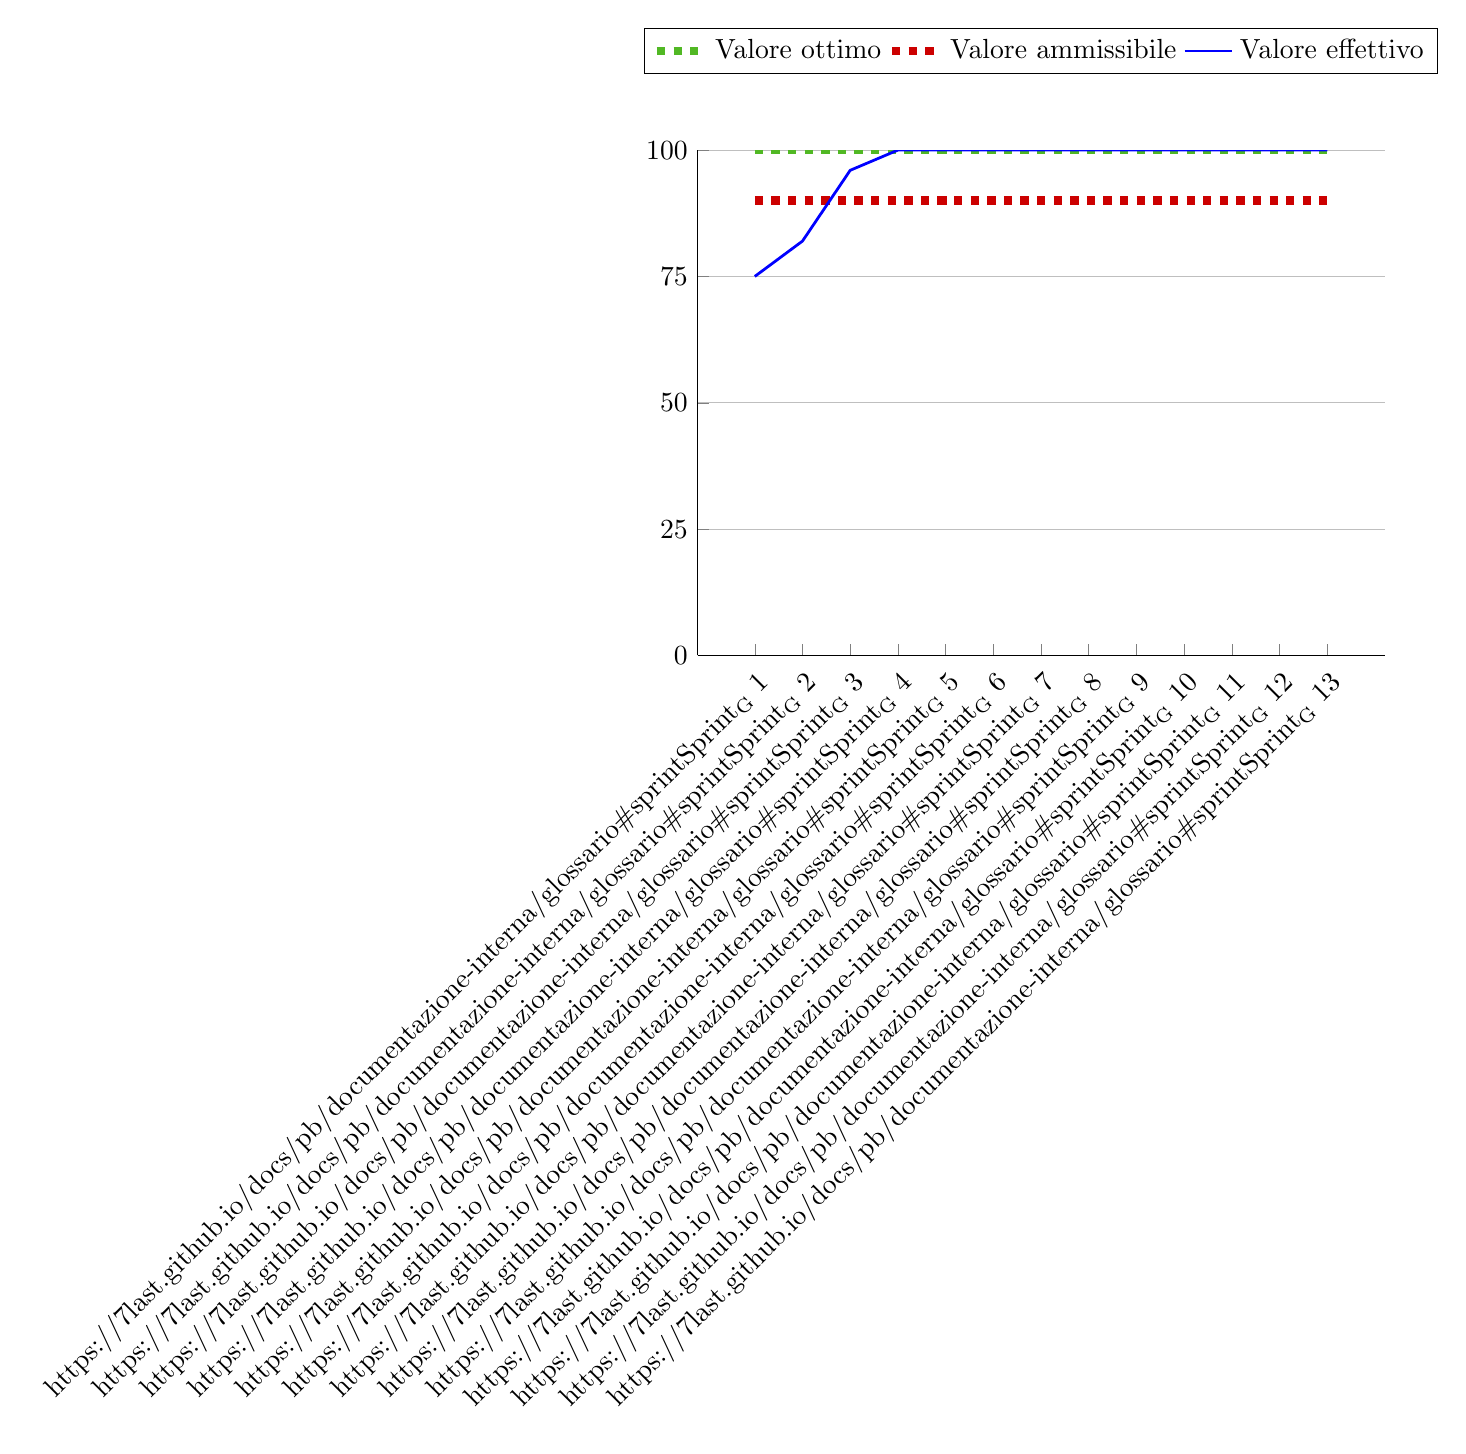
\begin{tikzpicture}
        \begin{axis}[
            width  = 0.85*\textwidth,
            height = 8cm,
            ymajorgrids = true,
            symbolic x coords={\href{https://7last.github.io/docs/pb/documentazione-interna/glossario\#sprint}{Sprint\textsubscript{G}} 1, \href{https://7last.github.io/docs/pb/documentazione-interna/glossario\#sprint}{Sprint\textsubscript{G}} 2, \href{https://7last.github.io/docs/pb/documentazione-interna/glossario\#sprint}{Sprint\textsubscript{G}} 3, \href{https://7last.github.io/docs/pb/documentazione-interna/glossario\#sprint}{Sprint\textsubscript{G}} 4, \href{https://7last.github.io/docs/pb/documentazione-interna/glossario\#sprint}{Sprint\textsubscript{G}} 5, \href{https://7last.github.io/docs/pb/documentazione-interna/glossario\#sprint}{Sprint\textsubscript{G}} 6, \href{https://7last.github.io/docs/pb/documentazione-interna/glossario\#sprint}{Sprint\textsubscript{G}} 7, \href{https://7last.github.io/docs/pb/documentazione-interna/glossario\#sprint}{Sprint\textsubscript{G}} 8, \href{https://7last.github.io/docs/pb/documentazione-interna/glossario\#sprint}{Sprint\textsubscript{G}} 9, \href{https://7last.github.io/docs/pb/documentazione-interna/glossario\#sprint}{Sprint\textsubscript{G}} 10, \href{https://7last.github.io/docs/pb/documentazione-interna/glossario\#sprint}{Sprint\textsubscript{G}} 11, \href{https://7last.github.io/docs/pb/documentazione-interna/glossario\#sprint}{Sprint\textsubscript{G}} 12, \href{https://7last.github.io/docs/pb/documentazione-interna/glossario\#sprint}{Sprint\textsubscript{G}} 13},
            xtick = data,
            ytick = {0, 25, 50, 75, 100},
            ymin=0, ymax=100,
            axis lines*=left,
            legend cell align=left,
            legend style={
                at={(0.5,1.15)},
                anchor=south,
                column sep=0.1ex,
                legend columns=3
            },
            xticklabel style={rotate=45, anchor=north east, yshift=0ex, xshift=0ex}
        ]
            \addplot[color=opt, style={dashed, line width=3pt}, mark=none] coordinates { % ottimo = 100
                (\href{https://7last.github.io/docs/pb/documentazione-interna/glossario\#sprint}{Sprint\textsubscript{G}} 1, 100)
                (\href{https://7last.github.io/docs/pb/documentazione-interna/glossario\#sprint}{Sprint\textsubscript{G}} 2, 100)
                (\href{https://7last.github.io/docs/pb/documentazione-interna/glossario\#sprint}{Sprint\textsubscript{G}} 3, 100)
                (\href{https://7last.github.io/docs/pb/documentazione-interna/glossario\#sprint}{Sprint\textsubscript{G}} 4, 100)
                (\href{https://7last.github.io/docs/pb/documentazione-interna/glossario\#sprint}{Sprint\textsubscript{G}} 5, 100)
                (\href{https://7last.github.io/docs/pb/documentazione-interna/glossario\#sprint}{Sprint\textsubscript{G}} 6, 100)
                (\href{https://7last.github.io/docs/pb/documentazione-interna/glossario\#sprint}{Sprint\textsubscript{G}} 7, 100)
                (\href{https://7last.github.io/docs/pb/documentazione-interna/glossario\#sprint}{Sprint\textsubscript{G}} 8, 100)
                (\href{https://7last.github.io/docs/pb/documentazione-interna/glossario\#sprint}{Sprint\textsubscript{G}} 9, 100)
                (\href{https://7last.github.io/docs/pb/documentazione-interna/glossario\#sprint}{Sprint\textsubscript{G}} 10, 100)
                (\href{https://7last.github.io/docs/pb/documentazione-interna/glossario\#sprint}{Sprint\textsubscript{G}} 11, 100)
                (\href{https://7last.github.io/docs/pb/documentazione-interna/glossario\#sprint}{Sprint\textsubscript{G}} 12, 100)
                (\href{https://7last.github.io/docs/pb/documentazione-interna/glossario\#sprint}{Sprint\textsubscript{G}} 13, 100)
            };
            \addplot[color=amm, style={dashed, line width=3pt}, mark=none] coordinates { % ammissibile = 90
                (\href{https://7last.github.io/docs/pb/documentazione-interna/glossario\#sprint}{Sprint\textsubscript{G}} 1, 90)
                (\href{https://7last.github.io/docs/pb/documentazione-interna/glossario\#sprint}{Sprint\textsubscript{G}} 2, 90)
                (\href{https://7last.github.io/docs/pb/documentazione-interna/glossario\#sprint}{Sprint\textsubscript{G}} 3, 90)
                (\href{https://7last.github.io/docs/pb/documentazione-interna/glossario\#sprint}{Sprint\textsubscript{G}} 4, 90)
                (\href{https://7last.github.io/docs/pb/documentazione-interna/glossario\#sprint}{Sprint\textsubscript{G}} 5, 90)
                (\href{https://7last.github.io/docs/pb/documentazione-interna/glossario\#sprint}{Sprint\textsubscript{G}} 6, 90)
                (\href{https://7last.github.io/docs/pb/documentazione-interna/glossario\#sprint}{Sprint\textsubscript{G}} 7, 90)
                (\href{https://7last.github.io/docs/pb/documentazione-interna/glossario\#sprint}{Sprint\textsubscript{G}} 8, 90)
                (\href{https://7last.github.io/docs/pb/documentazione-interna/glossario\#sprint}{Sprint\textsubscript{G}} 9, 90)
                (\href{https://7last.github.io/docs/pb/documentazione-interna/glossario\#sprint}{Sprint\textsubscript{G}} 10, 90)
                (\href{https://7last.github.io/docs/pb/documentazione-interna/glossario\#sprint}{Sprint\textsubscript{G}} 11, 90)
                (\href{https://7last.github.io/docs/pb/documentazione-interna/glossario\#sprint}{Sprint\textsubscript{G}} 12, 90)
                (\href{https://7last.github.io/docs/pb/documentazione-interna/glossario\#sprint}{Sprint\textsubscript{G}} 13, 90)
            };
            \addplot[color=blue, style={line width=1pt}, mark=none] coordinates {
                (\href{https://7last.github.io/docs/pb/documentazione-interna/glossario\#sprint}{Sprint\textsubscript{G}} 1, 75)
                (\href{https://7last.github.io/docs/pb/documentazione-interna/glossario\#sprint}{Sprint\textsubscript{G}} 2, 82)
                (\href{https://7last.github.io/docs/pb/documentazione-interna/glossario\#sprint}{Sprint\textsubscript{G}} 3, 96)
                (\href{https://7last.github.io/docs/pb/documentazione-interna/glossario\#sprint}{Sprint\textsubscript{G}} 4, 100)
                (\href{https://7last.github.io/docs/pb/documentazione-interna/glossario\#sprint}{Sprint\textsubscript{G}} 5, 100)
                (\href{https://7last.github.io/docs/pb/documentazione-interna/glossario\#sprint}{Sprint\textsubscript{G}} 6, 100)
                (\href{https://7last.github.io/docs/pb/documentazione-interna/glossario\#sprint}{Sprint\textsubscript{G}} 7, 100)
                (\href{https://7last.github.io/docs/pb/documentazione-interna/glossario\#sprint}{Sprint\textsubscript{G}} 8, 100)
                (\href{https://7last.github.io/docs/pb/documentazione-interna/glossario\#sprint}{Sprint\textsubscript{G}} 9, 100)
                (\href{https://7last.github.io/docs/pb/documentazione-interna/glossario\#sprint}{Sprint\textsubscript{G}} 10, 100)
                (\href{https://7last.github.io/docs/pb/documentazione-interna/glossario\#sprint}{Sprint\textsubscript{G}} 11, 100)
                (\href{https://7last.github.io/docs/pb/documentazione-interna/glossario\#sprint}{Sprint\textsubscript{G}} 12, 100)
                (\href{https://7last.github.io/docs/pb/documentazione-interna/glossario\#sprint}{Sprint\textsubscript{G}} 13, 100)
            };
            \legend{Valore ottimo, Valore ammissibile, Valore effettivo}
        \end{axis}
    \end{tikzpicture}
    \caption{Percentuale di metriche di qualità soddisfatte}
\end{figure*}
%--------- FINE GRAFICO -----------%
\begin{flushleft}
\href{https://7last.github.io/docs/pb/documentazione-interna/glossario\#requirements-and-technology-baseline}{\textbf{RTB}\textsubscript{G}} \\
Osservando il grafico si può notare come inizialmente il valore delle metriche soddisfatte sia inferiore al valore ammissibile, questo è dovuto principalmente all'inesperienza del team. Successivamente l'andamento cresce progressivamente fino ad arrivare al 100\% nell'ultimo \href{https://7last.github.io/docs/pb/documentazione-interna/glossario\#sprint}{sprint\textsubscript{G}}. Questo indica un miglioramento progressivo del \textit{Way of Working} del gruppo. \\
\href{https://7last.github.io/docs/pb/documentazione-interna/glossario\#product-baseline}{\textbf{PB}\textsubscript{G}} \\
Come si evince dal grafico, il \href{https://7last.github.io/docs/pb/documentazione-interna/glossario\#cruscotto}{cruscotto\textsubscript{G}} di valutazione della qualità ha permesso al gruppo di monitorare costantemente il soddisfacimento delle metriche di qualità, ottenendo così un miglioramento progressivo fino al raggiungimento del 100\% delle metriche soddisfatte.
\end{flushleft}

\newpage
\subsection{Qualità del processo di verifica}
\subsubsection{26M-CC - Code coverage}
%--------- GRAFICO -----------%
\begin{figure*}[!h]
    \centering
    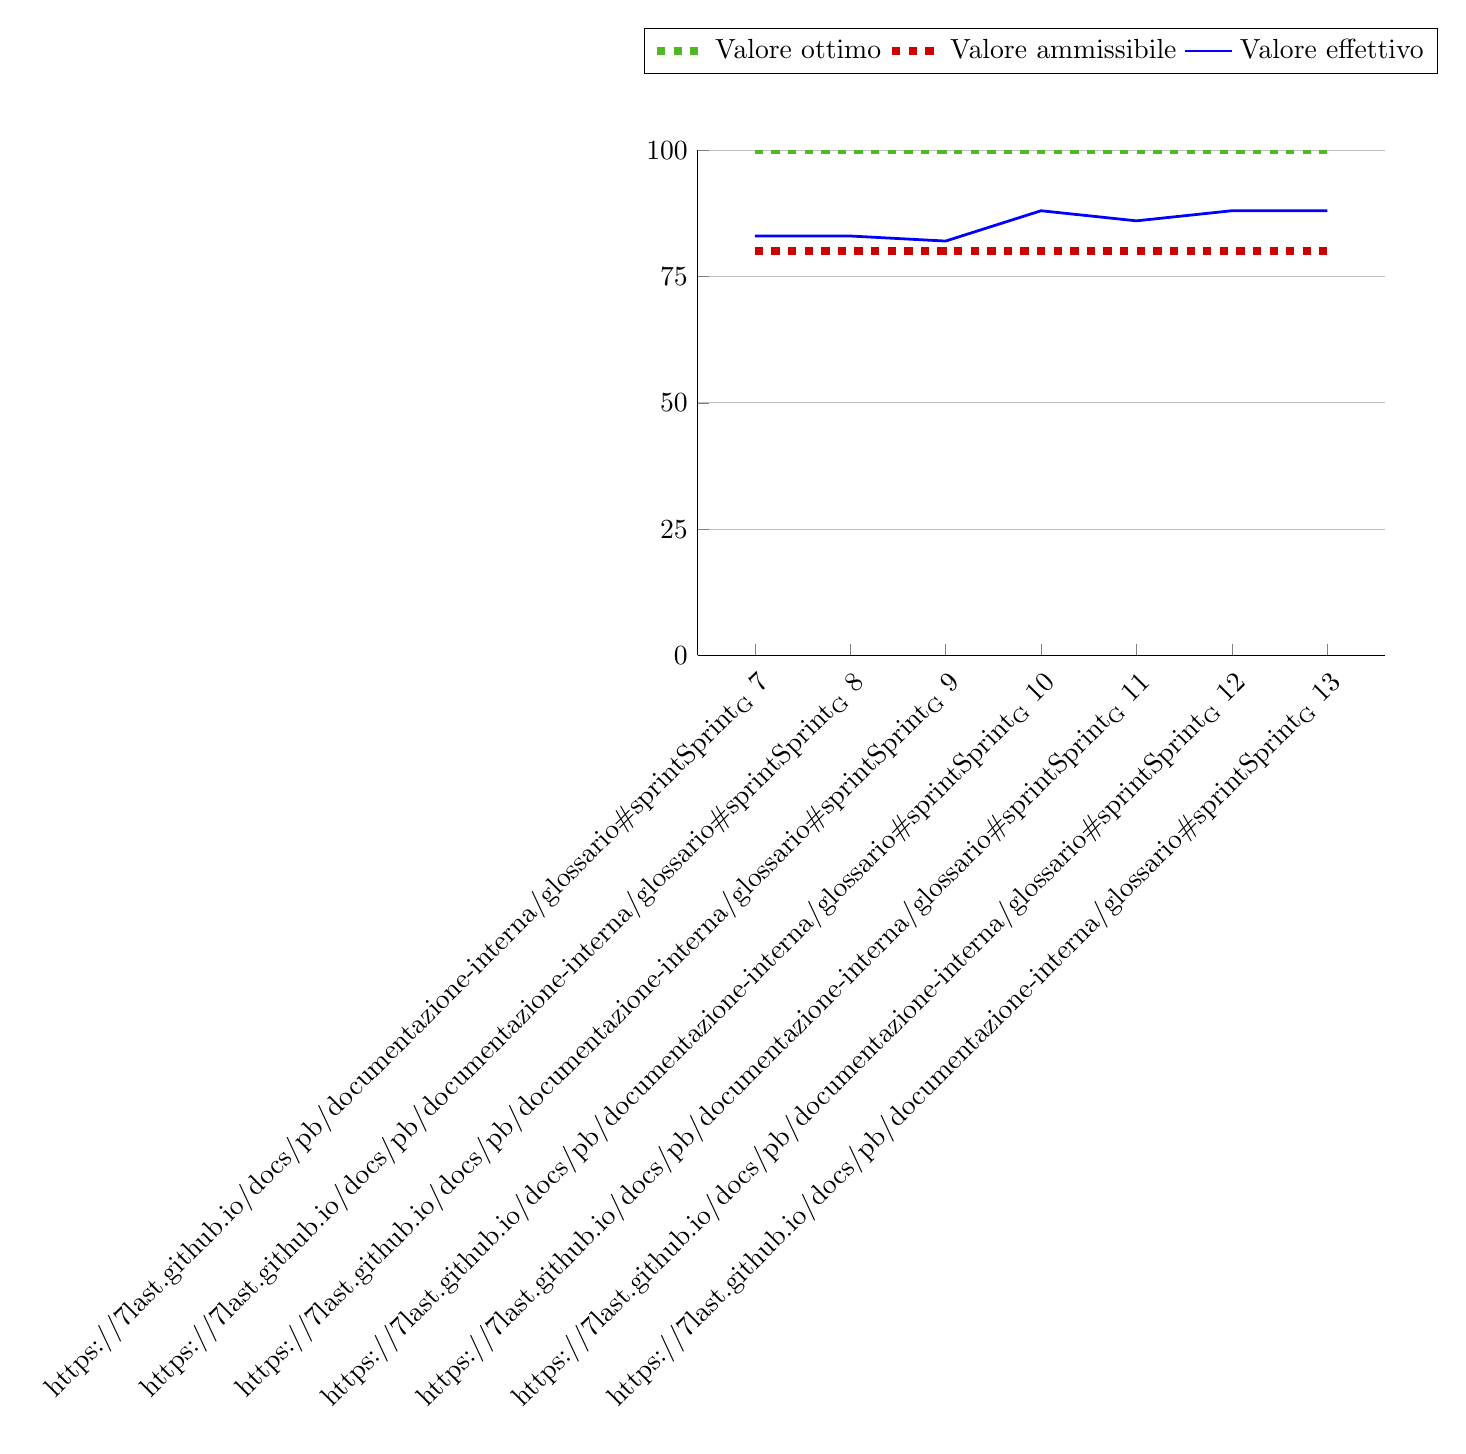
\begin{tikzpicture}
        \begin{axis}[
            width  = 0.85*\textwidth,
            height = 8cm,
            ymajorgrids = true,
            symbolic x coords={\href{https://7last.github.io/docs/pb/documentazione-interna/glossario\#sprint}{Sprint\textsubscript{G}} 7, \href{https://7last.github.io/docs/pb/documentazione-interna/glossario\#sprint}{Sprint\textsubscript{G}} 8, \href{https://7last.github.io/docs/pb/documentazione-interna/glossario\#sprint}{Sprint\textsubscript{G}} 9, \href{https://7last.github.io/docs/pb/documentazione-interna/glossario\#sprint}{Sprint\textsubscript{G}} 10, \href{https://7last.github.io/docs/pb/documentazione-interna/glossario\#sprint}{Sprint\textsubscript{G}} 11, \href{https://7last.github.io/docs/pb/documentazione-interna/glossario\#sprint}{Sprint\textsubscript{G}} 12, \href{https://7last.github.io/docs/pb/documentazione-interna/glossario\#sprint}{Sprint\textsubscript{G}} 13},
            xtick = data,
            ytick = {0, 25, 50, 75, 100},
            ymin=0, ymax=100,
            axis lines*=left,
            legend cell align=left,
            legend style={
                at={(0.5,1.15)},
                anchor=south,
                column sep=0.1ex,
                legend columns=-1
            },
            xticklabel style={rotate=45, anchor=north east, yshift=0ex, xshift=0ex}
            ]
            \addplot[color=opt, style={dashed, line width=3pt}, mark=none] coordinates {
                (\href{https://7last.github.io/docs/pb/documentazione-interna/glossario\#sprint}{Sprint\textsubscript{G}} 7, 100)
                (\href{https://7last.github.io/docs/pb/documentazione-interna/glossario\#sprint}{Sprint\textsubscript{G}} 8, 100)
                (\href{https://7last.github.io/docs/pb/documentazione-interna/glossario\#sprint}{Sprint\textsubscript{G}} 9, 100)
                (\href{https://7last.github.io/docs/pb/documentazione-interna/glossario\#sprint}{Sprint\textsubscript{G}} 10, 100)
                (\href{https://7last.github.io/docs/pb/documentazione-interna/glossario\#sprint}{Sprint\textsubscript{G}} 11, 100)
                (\href{https://7last.github.io/docs/pb/documentazione-interna/glossario\#sprint}{Sprint\textsubscript{G}} 12, 100)
                (\href{https://7last.github.io/docs/pb/documentazione-interna/glossario\#sprint}{Sprint\textsubscript{G}} 13, 100)
            };
            \addplot[color=amm, style={dashed, line width=3pt}, mark=none] coordinates {
                (\href{https://7last.github.io/docs/pb/documentazione-interna/glossario\#sprint}{Sprint\textsubscript{G}} 7, 80)
                (\href{https://7last.github.io/docs/pb/documentazione-interna/glossario\#sprint}{Sprint\textsubscript{G}} 8, 80)
                (\href{https://7last.github.io/docs/pb/documentazione-interna/glossario\#sprint}{Sprint\textsubscript{G}} 9, 80)
                (\href{https://7last.github.io/docs/pb/documentazione-interna/glossario\#sprint}{Sprint\textsubscript{G}} 10, 80)
                (\href{https://7last.github.io/docs/pb/documentazione-interna/glossario\#sprint}{Sprint\textsubscript{G}} 11, 80)
                (\href{https://7last.github.io/docs/pb/documentazione-interna/glossario\#sprint}{Sprint\textsubscript{G}} 12, 80)
                (\href{https://7last.github.io/docs/pb/documentazione-interna/glossario\#sprint}{Sprint\textsubscript{G}} 13, 80)
            };
            \addplot[color=blue, style={line width=1pt}, mark=none] coordinates {
                (\href{https://7last.github.io/docs/pb/documentazione-interna/glossario\#sprint}{Sprint\textsubscript{G}} 7, 83)
                (\href{https://7last.github.io/docs/pb/documentazione-interna/glossario\#sprint}{Sprint\textsubscript{G}} 8, 83)
                (\href{https://7last.github.io/docs/pb/documentazione-interna/glossario\#sprint}{Sprint\textsubscript{G}} 9, 82)
                (\href{https://7last.github.io/docs/pb/documentazione-interna/glossario\#sprint}{Sprint\textsubscript{G}} 10, 88)
                (\href{https://7last.github.io/docs/pb/documentazione-interna/glossario\#sprint}{Sprint\textsubscript{G}} 11, 86)
                (\href{https://7last.github.io/docs/pb/documentazione-interna/glossario\#sprint}{Sprint\textsubscript{G}} 12, 88)
                (\href{https://7last.github.io/docs/pb/documentazione-interna/glossario\#sprint}{Sprint\textsubscript{G}} 13, 88)
            };
            \legend{Valore ottimo, Valore ammissibile, Valore effettivo}
        \end{axis}
    \end{tikzpicture}
    \caption{Percentuale di code coverage dei test implementati}
\end{figure*}
%--------- FINE GRAFICO -----------% \\
\begin{flushleft}
\href{https://7last.github.io/docs/pb/documentazione-interna/glossario\#product-baseline}{\textbf{PB}\textsubscript{G}} \\
Al settimo \href{https://7last.github.io/docs/pb/documentazione-interna/glossario\#sprint}{sprint\textsubscript{G}} sono stati introdotti i primi test e fin da subito abbiamo voluto garantire la qualità del codice utilizzando le \href{https://7last.github.io/docs/pb/documentazione-interna/glossario\#github}{\textit{Github}\textsubscript{G}}\textit{ Actions} per impedire che venisse effettuato il \textit{merge} di codice non testato o che non superasse la percentuale minima prevista per ciascun test. Questo ha permesso di garantire un'alta percentuale di code coverage fin da subito, con un andamento costante e in crescita.
\end{flushleft}

\newpage
\subsubsection{27M-BC - Branch coverage}
%--------- GRAFICO -----------%
\begin{figure*}[!h]
    \centering
    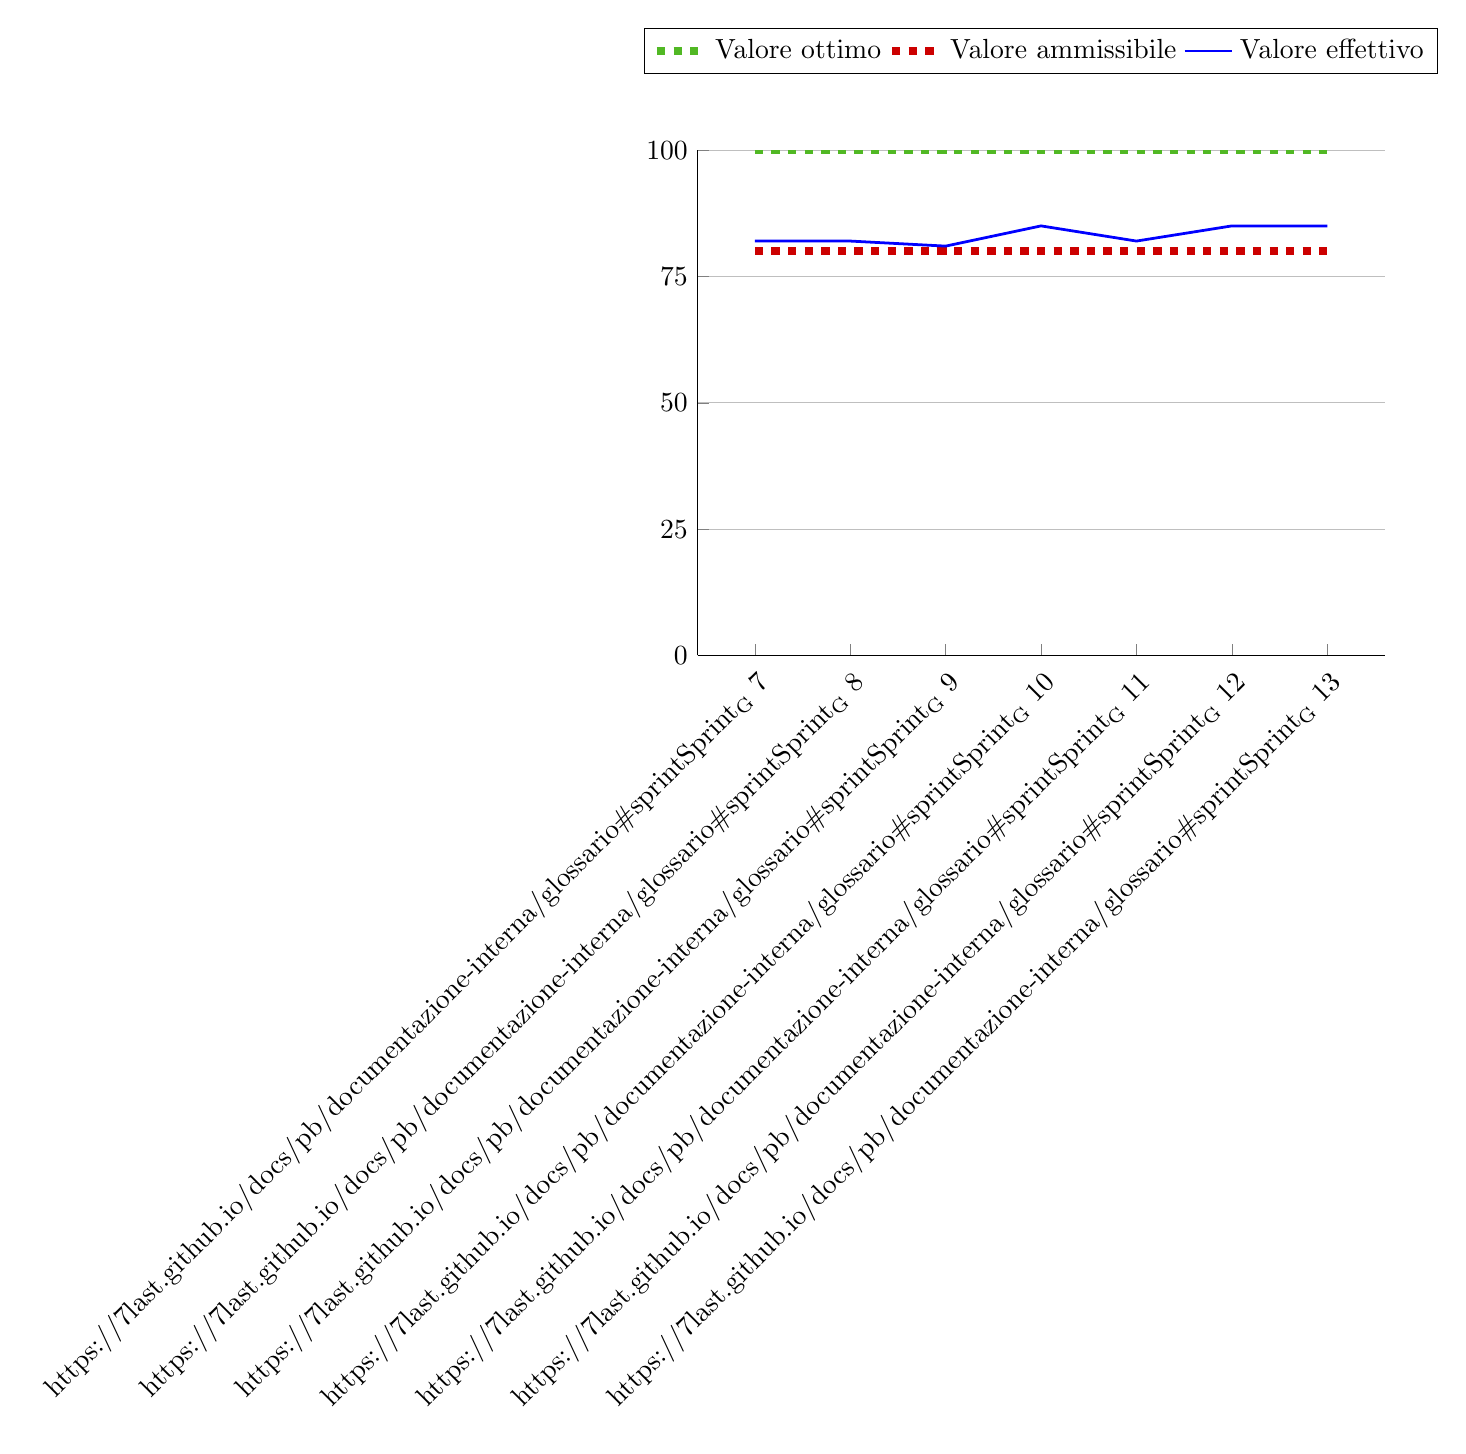
\begin{tikzpicture}
        \begin{axis}[
            width  = 0.85*\textwidth,
            height = 8cm,
            ymajorgrids = true,
            symbolic x coords={\href{https://7last.github.io/docs/pb/documentazione-interna/glossario\#sprint}{Sprint\textsubscript{G}} 7, \href{https://7last.github.io/docs/pb/documentazione-interna/glossario\#sprint}{Sprint\textsubscript{G}} 8, \href{https://7last.github.io/docs/pb/documentazione-interna/glossario\#sprint}{Sprint\textsubscript{G}} 9, \href{https://7last.github.io/docs/pb/documentazione-interna/glossario\#sprint}{Sprint\textsubscript{G}} 10, \href{https://7last.github.io/docs/pb/documentazione-interna/glossario\#sprint}{Sprint\textsubscript{G}} 11, \href{https://7last.github.io/docs/pb/documentazione-interna/glossario\#sprint}{Sprint\textsubscript{G}} 12, \href{https://7last.github.io/docs/pb/documentazione-interna/glossario\#sprint}{Sprint\textsubscript{G}} 13},
            xtick = data,
            ytick = {0, 25, 50, 75, 100},
            ymin=0, ymax=100,
            axis lines*=left,
            legend cell align=left,
            legend style={
                at={(0.5,1.15)},
                anchor=south,
                column sep=0.1ex,
                legend columns=3
            },
            xticklabel style={rotate=45, anchor=north east, yshift=0ex, xshift=0ex}
            ]
            \addplot[color=opt, style={dashed, line width=3pt}, mark=none] coordinates {
                (\href{https://7last.github.io/docs/pb/documentazione-interna/glossario\#sprint}{Sprint\textsubscript{G}} 7, 100)
                (\href{https://7last.github.io/docs/pb/documentazione-interna/glossario\#sprint}{Sprint\textsubscript{G}} 8, 100)
                (\href{https://7last.github.io/docs/pb/documentazione-interna/glossario\#sprint}{Sprint\textsubscript{G}} 9, 100)
                (\href{https://7last.github.io/docs/pb/documentazione-interna/glossario\#sprint}{Sprint\textsubscript{G}} 10, 100)
                (\href{https://7last.github.io/docs/pb/documentazione-interna/glossario\#sprint}{Sprint\textsubscript{G}} 11, 100)
                (\href{https://7last.github.io/docs/pb/documentazione-interna/glossario\#sprint}{Sprint\textsubscript{G}} 12, 100)
                (\href{https://7last.github.io/docs/pb/documentazione-interna/glossario\#sprint}{Sprint\textsubscript{G}} 13, 100)
            };
            \addplot[color=amm, style={dashed, line width=3pt}, mark=none] coordinates {
                (\href{https://7last.github.io/docs/pb/documentazione-interna/glossario\#sprint}{Sprint\textsubscript{G}} 7, 80)
                (\href{https://7last.github.io/docs/pb/documentazione-interna/glossario\#sprint}{Sprint\textsubscript{G}} 8, 80)
                (\href{https://7last.github.io/docs/pb/documentazione-interna/glossario\#sprint}{Sprint\textsubscript{G}} 9, 80)
                (\href{https://7last.github.io/docs/pb/documentazione-interna/glossario\#sprint}{Sprint\textsubscript{G}} 10, 80)
                (\href{https://7last.github.io/docs/pb/documentazione-interna/glossario\#sprint}{Sprint\textsubscript{G}} 11, 80)
                (\href{https://7last.github.io/docs/pb/documentazione-interna/glossario\#sprint}{Sprint\textsubscript{G}} 12, 80)
                (\href{https://7last.github.io/docs/pb/documentazione-interna/glossario\#sprint}{Sprint\textsubscript{G}} 13, 80)
            };
            \addplot[color=blue, style={line width=1pt}, mark=none] coordinates {
                (\href{https://7last.github.io/docs/pb/documentazione-interna/glossario\#sprint}{Sprint\textsubscript{G}} 7, 82)
                (\href{https://7last.github.io/docs/pb/documentazione-interna/glossario\#sprint}{Sprint\textsubscript{G}} 8, 82)
                (\href{https://7last.github.io/docs/pb/documentazione-interna/glossario\#sprint}{Sprint\textsubscript{G}} 9, 81)
                (\href{https://7last.github.io/docs/pb/documentazione-interna/glossario\#sprint}{Sprint\textsubscript{G}} 10, 85)
                (\href{https://7last.github.io/docs/pb/documentazione-interna/glossario\#sprint}{Sprint\textsubscript{G}} 11, 82)
                (\href{https://7last.github.io/docs/pb/documentazione-interna/glossario\#sprint}{Sprint\textsubscript{G}} 12, 85)
                (\href{https://7last.github.io/docs/pb/documentazione-interna/glossario\#sprint}{Sprint\textsubscript{G}} 13, 85)
            };
            \legend{Valore ottimo, Valore ammissibile, Valore effettivo}
        \end{axis}
    \end{tikzpicture}
    \caption{Percentuale di branch coverage dei test implementati}
\end{figure*}
%--------- FINE GRAFICO -----------% \\
\begin{flushleft}
\href{https://7last.github.io/docs/pb/documentazione-interna/glossario\#product-baseline}{\textbf{PB}\textsubscript{G}} \\
Anche in questo grafico si può notare come il gruppo \textit{7Last} abbia lavorato in modo costante per garantire la qualità del codice, con un'andamento costante e in crescita della percentuale di branch coverage. Come detto prima, questo è stato possibile grazie all'utilizzo delle \href{https://7last.github.io/docs/pb/documentazione-interna/glossario\#github}{\textit{GitHub}\textsubscript{G}}\textit{ Actions} per impedire il \textit{merge} di codice non testato o che non superasse la percentuale minima prevista per ciascun test.
\end{flushleft}

\newpage
\subsubsection{28M-SC - Statement coverage}
%--------- GRAFICO -----------%
\begin{figure*}[!h]
    \centering
    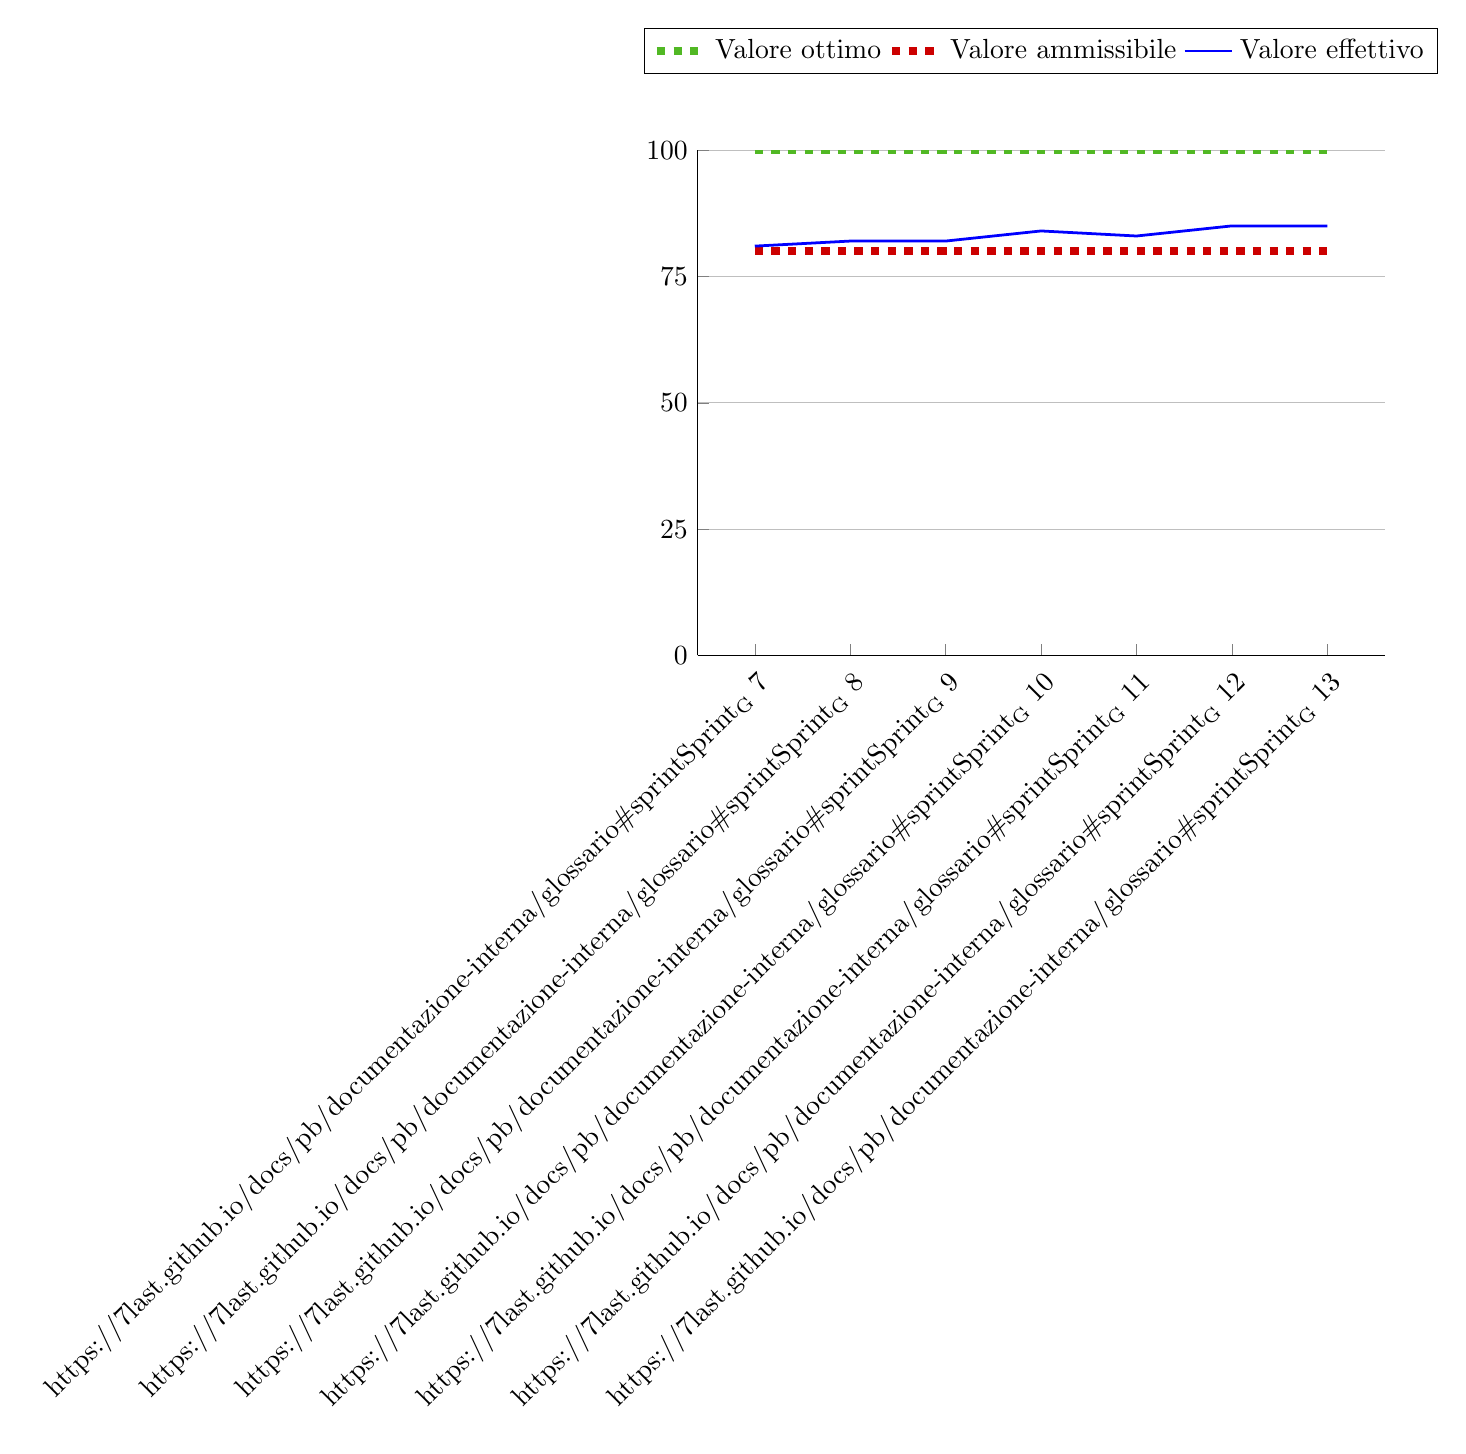
\begin{tikzpicture}
        \begin{axis}[
            width  = 0.85*\textwidth,
            height = 8cm,
            ymajorgrids = true,
            symbolic x coords={\href{https://7last.github.io/docs/pb/documentazione-interna/glossario\#sprint}{Sprint\textsubscript{G}} 7, \href{https://7last.github.io/docs/pb/documentazione-interna/glossario\#sprint}{Sprint\textsubscript{G}} 8, \href{https://7last.github.io/docs/pb/documentazione-interna/glossario\#sprint}{Sprint\textsubscript{G}} 9, \href{https://7last.github.io/docs/pb/documentazione-interna/glossario\#sprint}{Sprint\textsubscript{G}} 10, \href{https://7last.github.io/docs/pb/documentazione-interna/glossario\#sprint}{Sprint\textsubscript{G}} 11, \href{https://7last.github.io/docs/pb/documentazione-interna/glossario\#sprint}{Sprint\textsubscript{G}} 12, \href{https://7last.github.io/docs/pb/documentazione-interna/glossario\#sprint}{Sprint\textsubscript{G}} 13},
            xtick = data,
            ytick = {0, 25, 50, 75, 100},
            ymin=0, ymax=100,
            axis lines*=left,
            legend cell align=left,
            legend style={
                at={(0.5,1.15)},
                anchor=south,
                column sep=0.1ex,
                legend columns=3
            },
            xticklabel style={rotate=45, anchor=north east, yshift=0ex, xshift=0ex}
            ]
            \addplot[color=opt, style={dashed, line width=3pt}, mark=none] coordinates {
                (\href{https://7last.github.io/docs/pb/documentazione-interna/glossario\#sprint}{Sprint\textsubscript{G}} 7, 100)
                (\href{https://7last.github.io/docs/pb/documentazione-interna/glossario\#sprint}{Sprint\textsubscript{G}} 8, 100)
                (\href{https://7last.github.io/docs/pb/documentazione-interna/glossario\#sprint}{Sprint\textsubscript{G}} 9, 100)
                (\href{https://7last.github.io/docs/pb/documentazione-interna/glossario\#sprint}{Sprint\textsubscript{G}} 10, 100)
                (\href{https://7last.github.io/docs/pb/documentazione-interna/glossario\#sprint}{Sprint\textsubscript{G}} 11, 100)
                (\href{https://7last.github.io/docs/pb/documentazione-interna/glossario\#sprint}{Sprint\textsubscript{G}} 12, 100)
                (\href{https://7last.github.io/docs/pb/documentazione-interna/glossario\#sprint}{Sprint\textsubscript{G}} 13, 100)
            };
            \addplot[color=amm, style={dashed, line width=3pt}, mark=none] coordinates {
                (\href{https://7last.github.io/docs/pb/documentazione-interna/glossario\#sprint}{Sprint\textsubscript{G}} 7, 80)
                (\href{https://7last.github.io/docs/pb/documentazione-interna/glossario\#sprint}{Sprint\textsubscript{G}} 8, 80)
                (\href{https://7last.github.io/docs/pb/documentazione-interna/glossario\#sprint}{Sprint\textsubscript{G}} 9, 80)
                (\href{https://7last.github.io/docs/pb/documentazione-interna/glossario\#sprint}{Sprint\textsubscript{G}} 10, 80)
                (\href{https://7last.github.io/docs/pb/documentazione-interna/glossario\#sprint}{Sprint\textsubscript{G}} 11, 80)
                (\href{https://7last.github.io/docs/pb/documentazione-interna/glossario\#sprint}{Sprint\textsubscript{G}} 12, 80)
                (\href{https://7last.github.io/docs/pb/documentazione-interna/glossario\#sprint}{Sprint\textsubscript{G}} 13, 80)
            };
            \addplot[color=blue, style={line width=1pt}, mark=none] coordinates {
                (\href{https://7last.github.io/docs/pb/documentazione-interna/glossario\#sprint}{Sprint\textsubscript{G}} 7, 81)
                (\href{https://7last.github.io/docs/pb/documentazione-interna/glossario\#sprint}{Sprint\textsubscript{G}} 8, 82)
                (\href{https://7last.github.io/docs/pb/documentazione-interna/glossario\#sprint}{Sprint\textsubscript{G}} 9, 82) 
                (\href{https://7last.github.io/docs/pb/documentazione-interna/glossario\#sprint}{Sprint\textsubscript{G}} 10, 84)
                (\href{https://7last.github.io/docs/pb/documentazione-interna/glossario\#sprint}{Sprint\textsubscript{G}} 11, 83)
                (\href{https://7last.github.io/docs/pb/documentazione-interna/glossario\#sprint}{Sprint\textsubscript{G}} 12, 85)
                (\href{https://7last.github.io/docs/pb/documentazione-interna/glossario\#sprint}{Sprint\textsubscript{G}} 13, 85)
            };
            \legend{Valore ottimo, Valore ammissibile, Valore effettivo}
        \end{axis}
    \end{tikzpicture}
    \caption{Percentuale di statement coverage dei test implementati}
\end{figure*}
%--------- FINE GRAFICO -----------% \\
\begin{flushleft}
\href{https://7last.github.io/docs/pb/documentazione-interna/glossario\#product-baseline}{\textbf{PB}\textsubscript{G}} \\
Come già evidenziato in precedenza, anche qui abbiamo la conferma che il gruppo \textit{7Last} ha lavorato per garantire la qualità del codice, con un'andamento costante e in crescita della percentuale di statement coverage. Anche in questo caso, questo è stato possibile grazie all'utilizzo delle \href{https://7last.github.io/docs/pb/documentazione-interna/glossario\#github}{\textit{GitHub}\textsubscript{G}}\textit{ Actions} per impedire il \textit{merge} di codice non testato o che non superasse la percentuale minima prevista per ciascun test.
\end{flushleft}

\newpage
\subsubsection{29M-FD - Failure density}
%--------- GRAFICO -----------%
\begin{figure*}[!h]
    \centering
    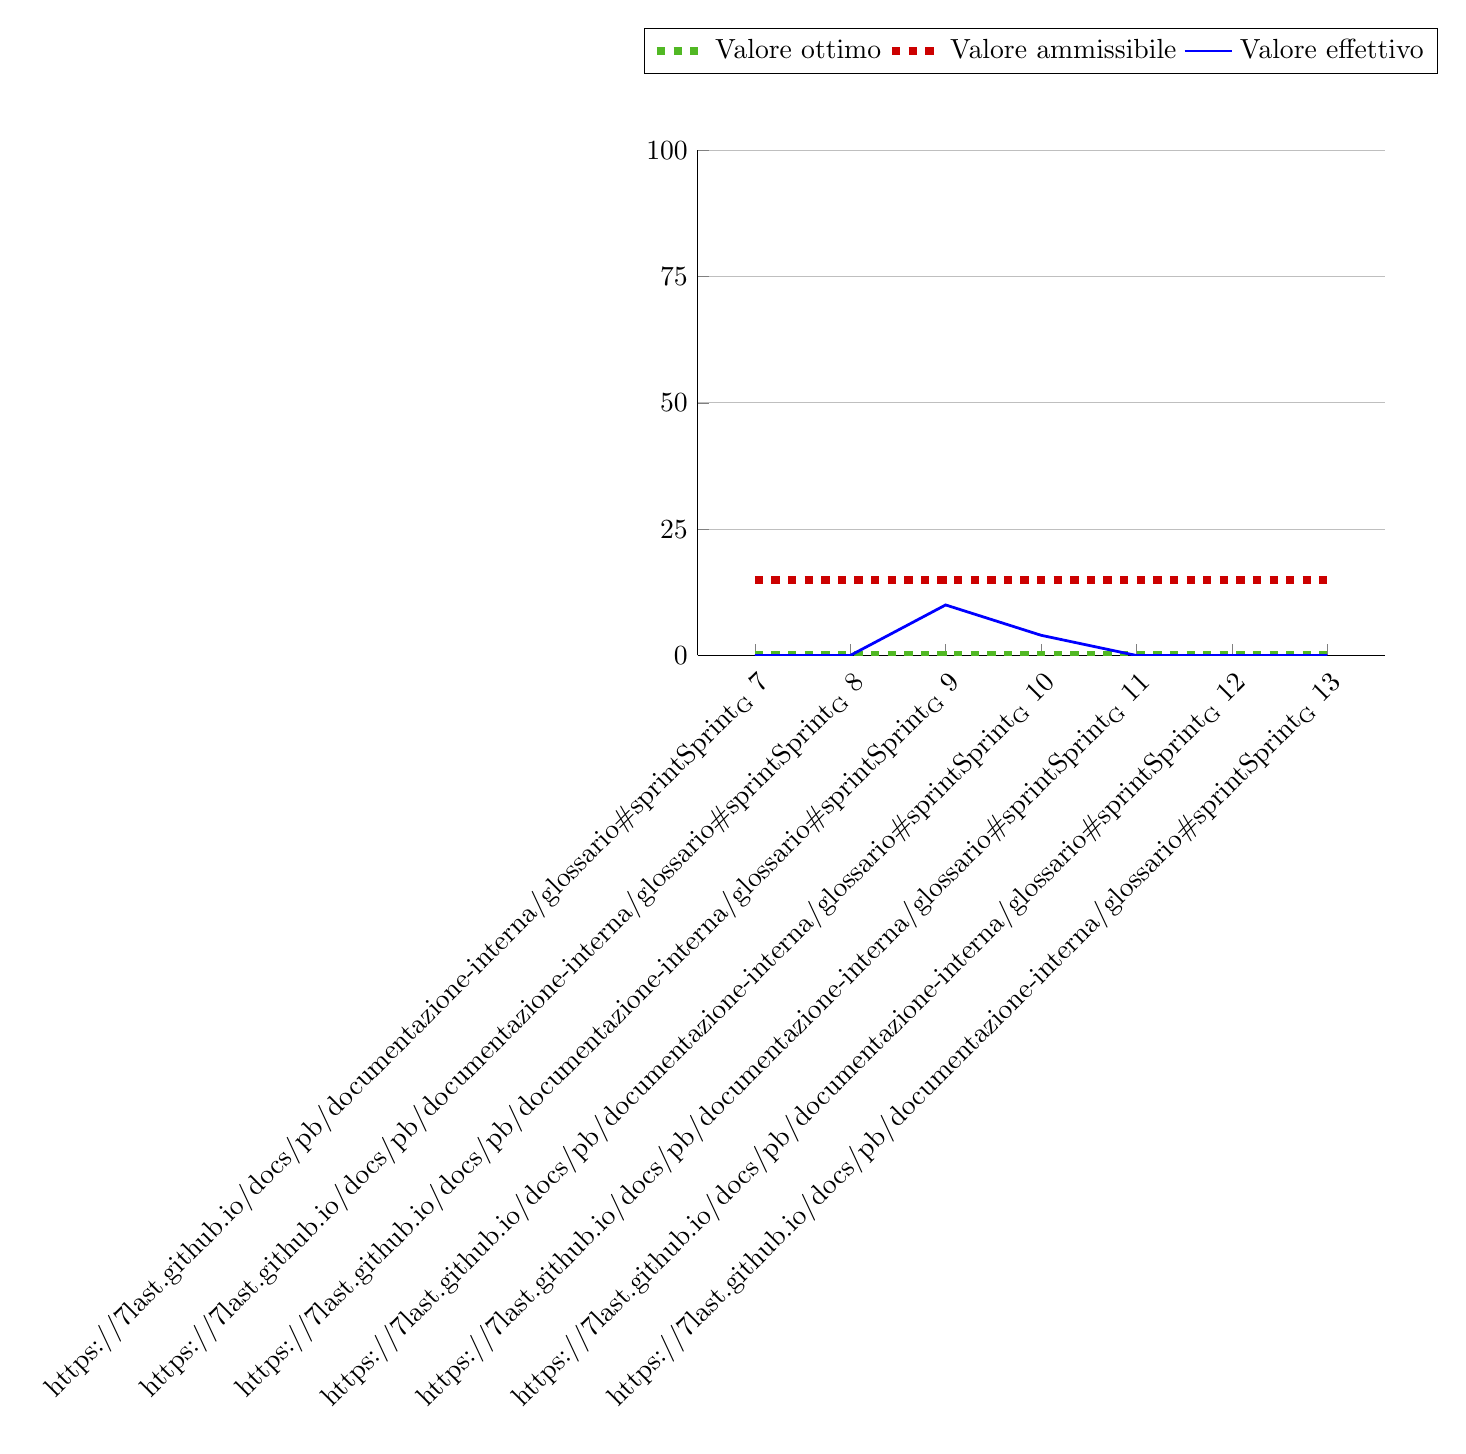
\begin{tikzpicture}
        \begin{axis}[
            width  = 0.85*\textwidth,
            height = 8cm,
            ymajorgrids = true,
            symbolic x coords={\href{https://7last.github.io/docs/pb/documentazione-interna/glossario\#sprint}{Sprint\textsubscript{G}} 7, \href{https://7last.github.io/docs/pb/documentazione-interna/glossario\#sprint}{Sprint\textsubscript{G}} 8, \href{https://7last.github.io/docs/pb/documentazione-interna/glossario\#sprint}{Sprint\textsubscript{G}} 9, \href{https://7last.github.io/docs/pb/documentazione-interna/glossario\#sprint}{Sprint\textsubscript{G}} 10, \href{https://7last.github.io/docs/pb/documentazione-interna/glossario\#sprint}{Sprint\textsubscript{G}} 11, \href{https://7last.github.io/docs/pb/documentazione-interna/glossario\#sprint}{Sprint\textsubscript{G}} 12, \href{https://7last.github.io/docs/pb/documentazione-interna/glossario\#sprint}{Sprint\textsubscript{G}} 13},
            xtick = data,
            ytick = {0, 25, 50, 75, 100},
            ymin=0, ymax=100,
            axis lines*=left,
            legend cell align=left,
            legend style={
                at={(0.5,1.15)},
                anchor=south,
                column sep=0.1ex,
                legend columns=3
            },
            xticklabel style={rotate=45, anchor=north east, yshift=0ex, xshift=0ex}
            ]
            \addplot[color=opt, style={dashed, line width=3pt}, mark=none] coordinates {
                (\href{https://7last.github.io/docs/pb/documentazione-interna/glossario\#sprint}{Sprint\textsubscript{G}} 7, 0)
                (\href{https://7last.github.io/docs/pb/documentazione-interna/glossario\#sprint}{Sprint\textsubscript{G}} 8, 0)
                (\href{https://7last.github.io/docs/pb/documentazione-interna/glossario\#sprint}{Sprint\textsubscript{G}} 9, 0)
                (\href{https://7last.github.io/docs/pb/documentazione-interna/glossario\#sprint}{Sprint\textsubscript{G}} 10, 0)
                (\href{https://7last.github.io/docs/pb/documentazione-interna/glossario\#sprint}{Sprint\textsubscript{G}} 11, 0)
                (\href{https://7last.github.io/docs/pb/documentazione-interna/glossario\#sprint}{Sprint\textsubscript{G}} 12, 0)
                (\href{https://7last.github.io/docs/pb/documentazione-interna/glossario\#sprint}{Sprint\textsubscript{G}} 13, 0)
            };
            \addplot[color=amm, style={dashed, line width=3pt}, mark=none] coordinates {
                (\href{https://7last.github.io/docs/pb/documentazione-interna/glossario\#sprint}{Sprint\textsubscript{G}} 7, 15)
                (\href{https://7last.github.io/docs/pb/documentazione-interna/glossario\#sprint}{Sprint\textsubscript{G}} 8, 15)
                (\href{https://7last.github.io/docs/pb/documentazione-interna/glossario\#sprint}{Sprint\textsubscript{G}} 9, 15)
                (\href{https://7last.github.io/docs/pb/documentazione-interna/glossario\#sprint}{Sprint\textsubscript{G}} 10, 15)
                (\href{https://7last.github.io/docs/pb/documentazione-interna/glossario\#sprint}{Sprint\textsubscript{G}} 11, 15)
                (\href{https://7last.github.io/docs/pb/documentazione-interna/glossario\#sprint}{Sprint\textsubscript{G}} 12, 15)
                (\href{https://7last.github.io/docs/pb/documentazione-interna/glossario\#sprint}{Sprint\textsubscript{G}} 13, 15)
            };
            \addplot[color=blue, style={line width=1pt}, mark=none] coordinates {
                (\href{https://7last.github.io/docs/pb/documentazione-interna/glossario\#sprint}{Sprint\textsubscript{G}} 7, 0)
                (\href{https://7last.github.io/docs/pb/documentazione-interna/glossario\#sprint}{Sprint\textsubscript{G}} 8, 0)
                (\href{https://7last.github.io/docs/pb/documentazione-interna/glossario\#sprint}{Sprint\textsubscript{G}} 9, 10)
                (\href{https://7last.github.io/docs/pb/documentazione-interna/glossario\#sprint}{Sprint\textsubscript{G}} 10, 4)
                (\href{https://7last.github.io/docs/pb/documentazione-interna/glossario\#sprint}{Sprint\textsubscript{G}} 11, 0)
                (\href{https://7last.github.io/docs/pb/documentazione-interna/glossario\#sprint}{Sprint\textsubscript{G}} 12, 0)
                (\href{https://7last.github.io/docs/pb/documentazione-interna/glossario\#sprint}{Sprint\textsubscript{G}} 13, 0)
            };
            \legend{Valore ottimo, Valore ammissibile, Valore effettivo}
        \end{axis}
    \end{tikzpicture}
    \caption{Percentuale di failure density}
\end{figure*}
%--------- FINE GRAFICO -----------% \\
\begin{flushleft}
\href{https://7last.github.io/docs/pb/documentazione-interna/glossario\#product-baseline}{\textbf{PB}\textsubscript{G}} \\
Dal grafico risultano evidenti i primi fallimenti rilevati in corrispondenza del nono \href{https://7last.github.io/docs/pb/documentazione-interna/glossario\#sprint}{sprint\textsubscript{G}}, naturale conseguenza dell'aggiunta di nuovi test che hanno permesso di rilevare errori non precedentemente individuati e correggerli. Successivamente si nota un calo dei fallimenti fino al raggiungimento del valore ottimo.
\end{flushleft}

\newpage
\subsubsection{30M-PTCP - Passed test case percentage}
%--------- GRAFICO -----------%
\begin{figure*}[!h]
    \centering
    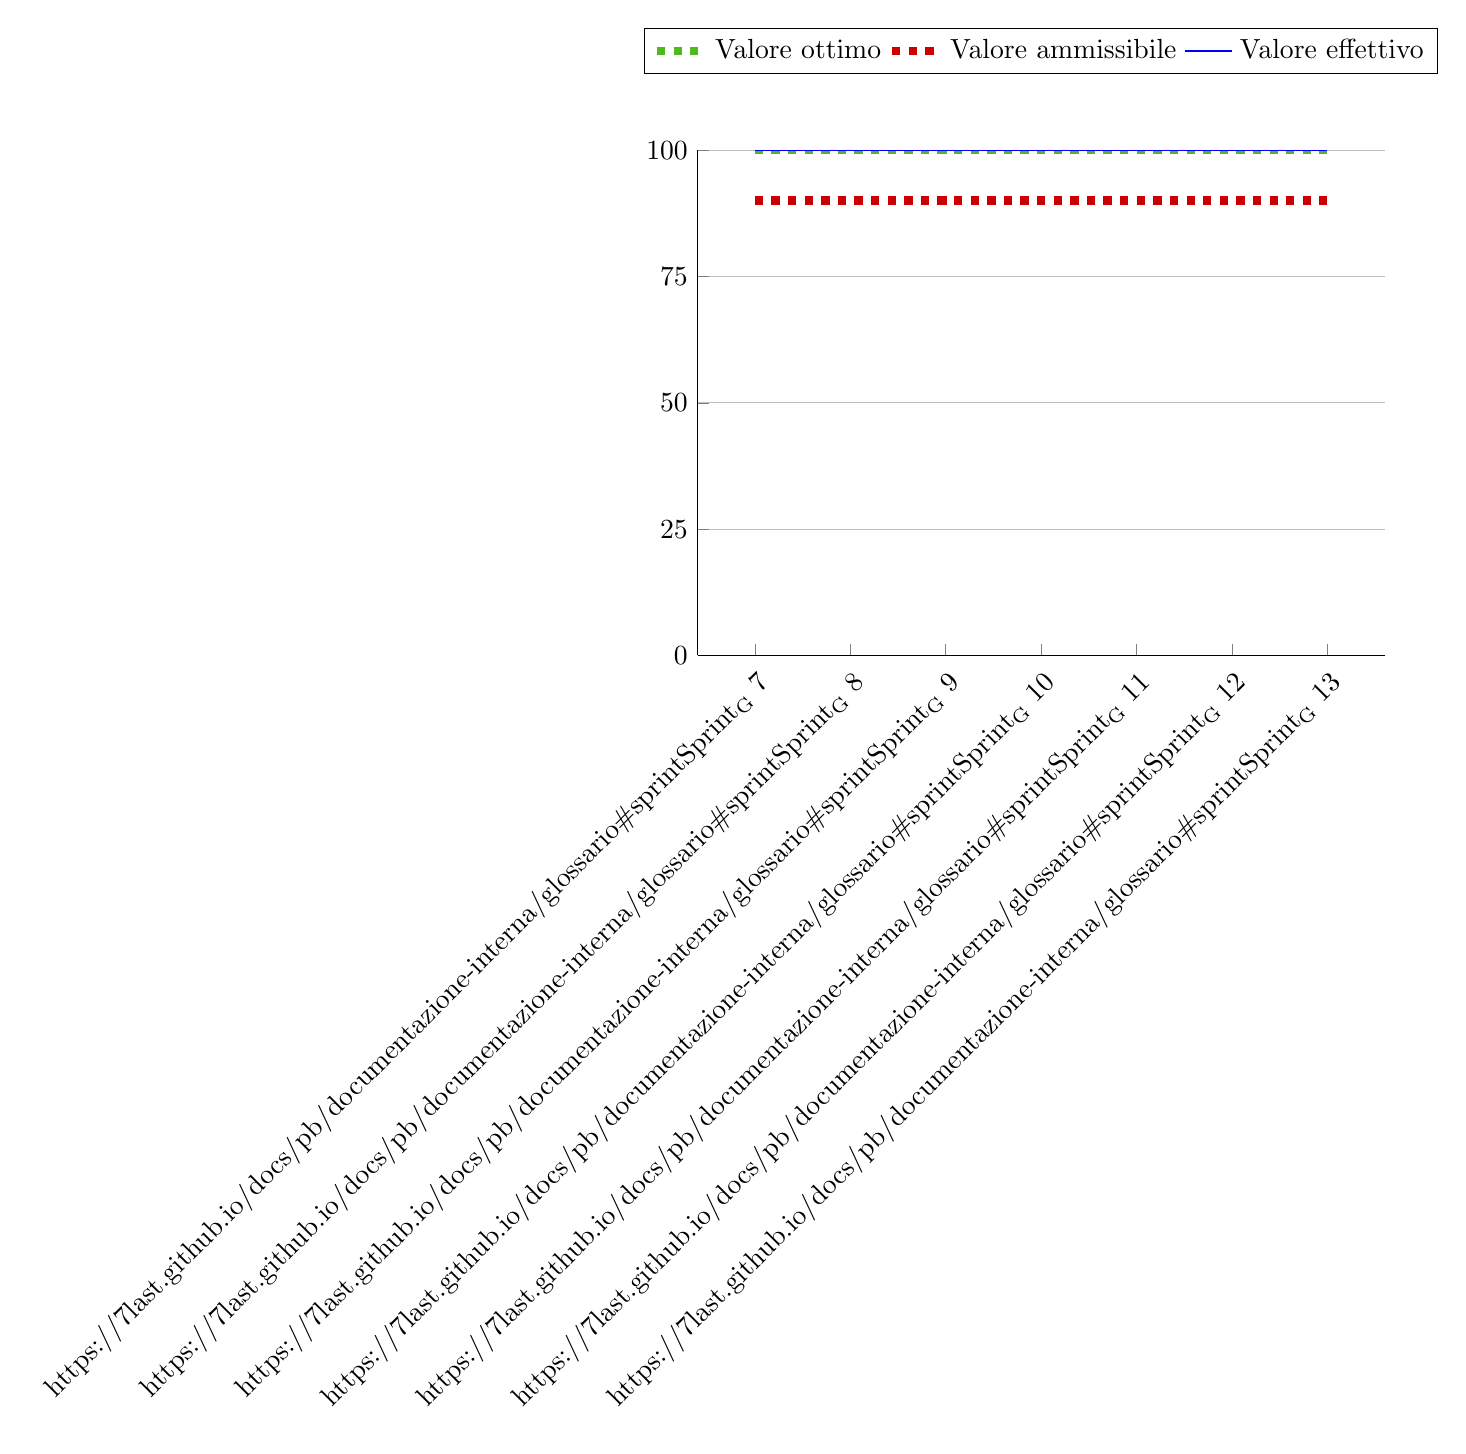
\begin{tikzpicture}
        \begin{axis}[
            width  = 0.85*\textwidth,
            height = 8cm,
            ymajorgrids = true,
            symbolic x coords={\href{https://7last.github.io/docs/pb/documentazione-interna/glossario\#sprint}{Sprint\textsubscript{G}} 7, \href{https://7last.github.io/docs/pb/documentazione-interna/glossario\#sprint}{Sprint\textsubscript{G}} 8, \href{https://7last.github.io/docs/pb/documentazione-interna/glossario\#sprint}{Sprint\textsubscript{G}} 9, \href{https://7last.github.io/docs/pb/documentazione-interna/glossario\#sprint}{Sprint\textsubscript{G}} 10, \href{https://7last.github.io/docs/pb/documentazione-interna/glossario\#sprint}{Sprint\textsubscript{G}} 11, \href{https://7last.github.io/docs/pb/documentazione-interna/glossario\#sprint}{Sprint\textsubscript{G}} 12, \href{https://7last.github.io/docs/pb/documentazione-interna/glossario\#sprint}{Sprint\textsubscript{G}} 13},
            xtick = data,
            ytick = {0, 25, 50, 75, 100},
            ymin=0, ymax=100,
            axis lines*=left,
            legend cell align=left,
            legend style={
                at={(0.5,1.15)},
                anchor=south,
                column sep=0.1ex,
                legend columns=3
            },
            xticklabel style={rotate=45, anchor=north east, yshift=0ex, xshift=0ex}
            ]
            \addplot[color=opt, style={dashed, line width=3pt}, mark=none] coordinates {
                (\href{https://7last.github.io/docs/pb/documentazione-interna/glossario\#sprint}{Sprint\textsubscript{G}} 7, 100)
                (\href{https://7last.github.io/docs/pb/documentazione-interna/glossario\#sprint}{Sprint\textsubscript{G}} 8, 100)
                (\href{https://7last.github.io/docs/pb/documentazione-interna/glossario\#sprint}{Sprint\textsubscript{G}} 9, 100)
                (\href{https://7last.github.io/docs/pb/documentazione-interna/glossario\#sprint}{Sprint\textsubscript{G}} 10, 100)
                (\href{https://7last.github.io/docs/pb/documentazione-interna/glossario\#sprint}{Sprint\textsubscript{G}} 11, 100)
                (\href{https://7last.github.io/docs/pb/documentazione-interna/glossario\#sprint}{Sprint\textsubscript{G}} 12, 100)
                (\href{https://7last.github.io/docs/pb/documentazione-interna/glossario\#sprint}{Sprint\textsubscript{G}} 13, 100)
            };
            \addplot[color=amm, style={dashed, line width=3pt}, mark=none] coordinates {
                (\href{https://7last.github.io/docs/pb/documentazione-interna/glossario\#sprint}{Sprint\textsubscript{G}} 7, 90)
                (\href{https://7last.github.io/docs/pb/documentazione-interna/glossario\#sprint}{Sprint\textsubscript{G}} 8, 90)
                (\href{https://7last.github.io/docs/pb/documentazione-interna/glossario\#sprint}{Sprint\textsubscript{G}} 9, 90)
                (\href{https://7last.github.io/docs/pb/documentazione-interna/glossario\#sprint}{Sprint\textsubscript{G}} 10, 90)
                (\href{https://7last.github.io/docs/pb/documentazione-interna/glossario\#sprint}{Sprint\textsubscript{G}} 11, 90)
                (\href{https://7last.github.io/docs/pb/documentazione-interna/glossario\#sprint}{Sprint\textsubscript{G}} 12, 90)
                (\href{https://7last.github.io/docs/pb/documentazione-interna/glossario\#sprint}{Sprint\textsubscript{G}} 13, 90)
            };
            \addplot[color=blue, style={line width=1pt}, mark=none] coordinates {
                (\href{https://7last.github.io/docs/pb/documentazione-interna/glossario\#sprint}{Sprint\textsubscript{G}} 7, 100)
                (\href{https://7last.github.io/docs/pb/documentazione-interna/glossario\#sprint}{Sprint\textsubscript{G}} 8, 100)
                (\href{https://7last.github.io/docs/pb/documentazione-interna/glossario\#sprint}{Sprint\textsubscript{G}} 9, 100)
                (\href{https://7last.github.io/docs/pb/documentazione-interna/glossario\#sprint}{Sprint\textsubscript{G}} 10, 100)
                (\href{https://7last.github.io/docs/pb/documentazione-interna/glossario\#sprint}{Sprint\textsubscript{G}} 11, 100)
                (\href{https://7last.github.io/docs/pb/documentazione-interna/glossario\#sprint}{Sprint\textsubscript{G}} 12, 100)
                (\href{https://7last.github.io/docs/pb/documentazione-interna/glossario\#sprint}{Sprint\textsubscript{G}} 13, 100)
            };
            \legend{Valore ottimo, Valore ammissibile, Valore effettivo}
        \end{axis}
    \end{tikzpicture}
    \caption{Percentuale di casi di test superati}
\end{figure*}
%--------- FINE GRAFICO -----------% \\
\begin{flushleft}
\href{https://7last.github.io/docs/pb/documentazione-interna/glossario\#product-baseline}{\textbf{PB}\textsubscript{G}} \\
Grazie all'utilizzo delle \href{https://7last.github.io/docs/pb/documentazione-interna/glossario\#github}{\textit{GitHub}\textsubscript{G}}\textit{ Actions}, il gruppo \textit{7Last} è riuscito a garantire che tutti i test implementati venissero superati, con un'andamento costante fisso al 100\% già dall'implementazione dei primi test in corrispondenza del settimo \href{https://7last.github.io/docs/pb/documentazione-interna/glossario\#sprint}{sprint\textsubscript{G}} fino alla fine del progetto.
\end{flushleft}

\newpage
\subsection{Qualità del processo di gestione dei rischi}
\subsubsection{32M-NCR - Rischi non calcolati}
%--------- GRAFICO -----------%
\begin{figure*}[!h]
    \centering
    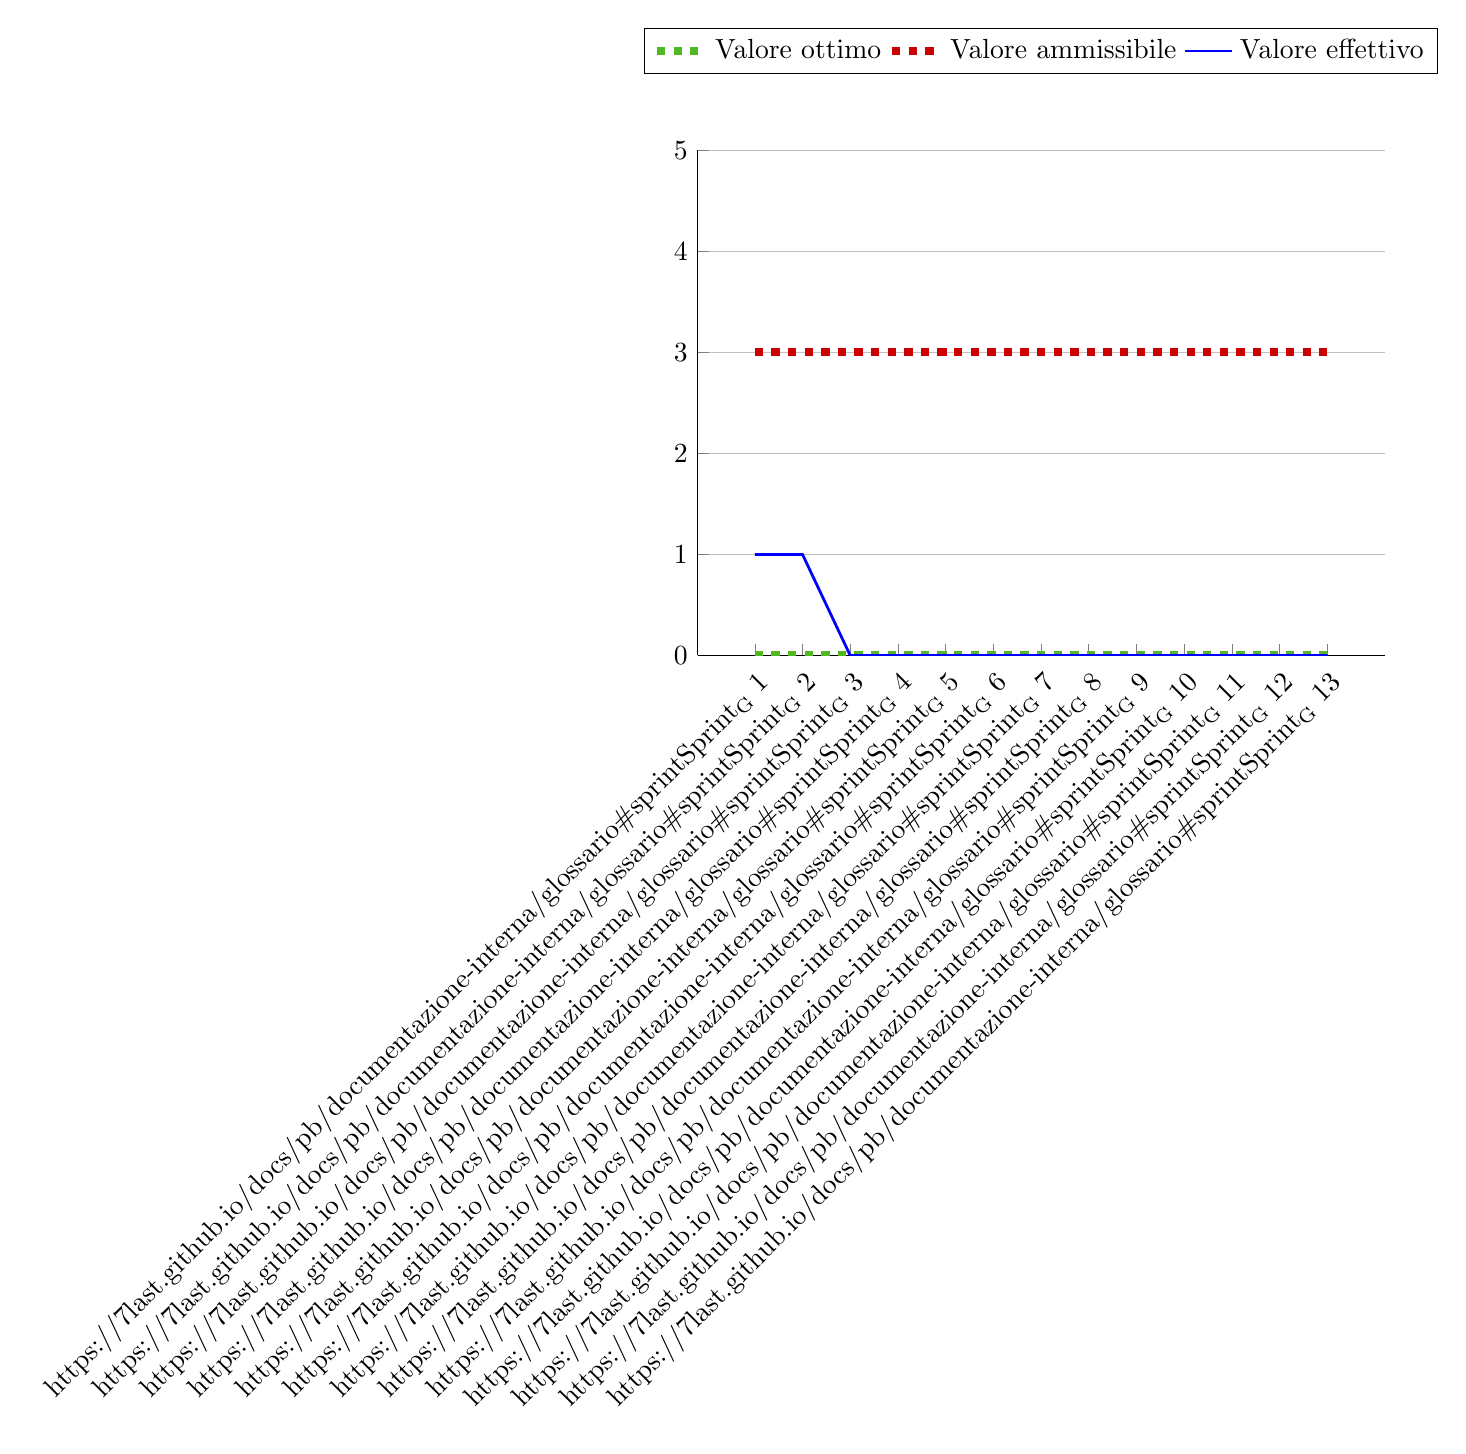
\begin{tikzpicture}
        \begin{axis}[
            width  = 0.85*\textwidth,
            height = 8cm,
            ymajorgrids = true,
            symbolic x coords={\href{https://7last.github.io/docs/pb/documentazione-interna/glossario\#sprint}{Sprint\textsubscript{G}} 1, \href{https://7last.github.io/docs/pb/documentazione-interna/glossario\#sprint}{Sprint\textsubscript{G}} 2, \href{https://7last.github.io/docs/pb/documentazione-interna/glossario\#sprint}{Sprint\textsubscript{G}} 3, \href{https://7last.github.io/docs/pb/documentazione-interna/glossario\#sprint}{Sprint\textsubscript{G}} 4, \href{https://7last.github.io/docs/pb/documentazione-interna/glossario\#sprint}{Sprint\textsubscript{G}} 5, \href{https://7last.github.io/docs/pb/documentazione-interna/glossario\#sprint}{Sprint\textsubscript{G}} 6, \href{https://7last.github.io/docs/pb/documentazione-interna/glossario\#sprint}{Sprint\textsubscript{G}} 7, \href{https://7last.github.io/docs/pb/documentazione-interna/glossario\#sprint}{Sprint\textsubscript{G}} 8, \href{https://7last.github.io/docs/pb/documentazione-interna/glossario\#sprint}{Sprint\textsubscript{G}} 9, \href{https://7last.github.io/docs/pb/documentazione-interna/glossario\#sprint}{Sprint\textsubscript{G}} 10, \href{https://7last.github.io/docs/pb/documentazione-interna/glossario\#sprint}{Sprint\textsubscript{G}} 11, \href{https://7last.github.io/docs/pb/documentazione-interna/glossario\#sprint}{Sprint\textsubscript{G}} 12, \href{https://7last.github.io/docs/pb/documentazione-interna/glossario\#sprint}{Sprint\textsubscript{G}} 13},
            xtick = data,
            ymin=0, ymax=5,
            axis lines*=left,
            legend cell align=left,
            legend style={
                at={(0.5,1.15)},
                anchor=south,
                column sep=0.1ex,
                legend columns=3
            },
            xticklabel style={rotate=45, anchor=north east, yshift=0ex, xshift=0ex}
        ]
            \addplot[color=opt, style={dashed, line width=3pt}, mark=none] coordinates { % ottimo = 0
                (\href{https://7last.github.io/docs/pb/documentazione-interna/glossario\#sprint}{Sprint\textsubscript{G}} 1, 0)
                (\href{https://7last.github.io/docs/pb/documentazione-interna/glossario\#sprint}{Sprint\textsubscript{G}} 2, 0)
                (\href{https://7last.github.io/docs/pb/documentazione-interna/glossario\#sprint}{Sprint\textsubscript{G}} 3, 0)
                (\href{https://7last.github.io/docs/pb/documentazione-interna/glossario\#sprint}{Sprint\textsubscript{G}} 4, 0)
                (\href{https://7last.github.io/docs/pb/documentazione-interna/glossario\#sprint}{Sprint\textsubscript{G}} 5, 0)
                (\href{https://7last.github.io/docs/pb/documentazione-interna/glossario\#sprint}{Sprint\textsubscript{G}} 6, 0)
                (\href{https://7last.github.io/docs/pb/documentazione-interna/glossario\#sprint}{Sprint\textsubscript{G}} 7, 0)
                (\href{https://7last.github.io/docs/pb/documentazione-interna/glossario\#sprint}{Sprint\textsubscript{G}} 8, 0)
                (\href{https://7last.github.io/docs/pb/documentazione-interna/glossario\#sprint}{Sprint\textsubscript{G}} 9, 0)
                (\href{https://7last.github.io/docs/pb/documentazione-interna/glossario\#sprint}{Sprint\textsubscript{G}} 10, 0)
                (\href{https://7last.github.io/docs/pb/documentazione-interna/glossario\#sprint}{Sprint\textsubscript{G}} 11, 0)
                (\href{https://7last.github.io/docs/pb/documentazione-interna/glossario\#sprint}{Sprint\textsubscript{G}} 12, 0)
                (\href{https://7last.github.io/docs/pb/documentazione-interna/glossario\#sprint}{Sprint\textsubscript{G}} 13, 0)
            };
            \addplot[color=amm, style={dashed, line width=3pt}, mark=none] coordinates { % ammissibile = 3
                (\href{https://7last.github.io/docs/pb/documentazione-interna/glossario\#sprint}{Sprint\textsubscript{G}} 1, 3)
                (\href{https://7last.github.io/docs/pb/documentazione-interna/glossario\#sprint}{Sprint\textsubscript{G}} 2, 3)
                (\href{https://7last.github.io/docs/pb/documentazione-interna/glossario\#sprint}{Sprint\textsubscript{G}} 3, 3)
                (\href{https://7last.github.io/docs/pb/documentazione-interna/glossario\#sprint}{Sprint\textsubscript{G}} 4, 3)
                (\href{https://7last.github.io/docs/pb/documentazione-interna/glossario\#sprint}{Sprint\textsubscript{G}} 5, 3)
                (\href{https://7last.github.io/docs/pb/documentazione-interna/glossario\#sprint}{Sprint\textsubscript{G}} 6, 3)
                (\href{https://7last.github.io/docs/pb/documentazione-interna/glossario\#sprint}{Sprint\textsubscript{G}} 7, 3)
                (\href{https://7last.github.io/docs/pb/documentazione-interna/glossario\#sprint}{Sprint\textsubscript{G}} 8, 3)
                (\href{https://7last.github.io/docs/pb/documentazione-interna/glossario\#sprint}{Sprint\textsubscript{G}} 9, 3)
                (\href{https://7last.github.io/docs/pb/documentazione-interna/glossario\#sprint}{Sprint\textsubscript{G}} 10, 3)
                (\href{https://7last.github.io/docs/pb/documentazione-interna/glossario\#sprint}{Sprint\textsubscript{G}} 11, 3)
                (\href{https://7last.github.io/docs/pb/documentazione-interna/glossario\#sprint}{Sprint\textsubscript{G}} 12, 3)
                (\href{https://7last.github.io/docs/pb/documentazione-interna/glossario\#sprint}{Sprint\textsubscript{G}} 13, 3)
            };
            \addplot[color=blue, style={line width=1pt}, mark=none] coordinates { % rischi non calcolati
                (\href{https://7last.github.io/docs/pb/documentazione-interna/glossario\#sprint}{Sprint\textsubscript{G}} 1, 1)
                (\href{https://7last.github.io/docs/pb/documentazione-interna/glossario\#sprint}{Sprint\textsubscript{G}} 2, 1)
                (\href{https://7last.github.io/docs/pb/documentazione-interna/glossario\#sprint}{Sprint\textsubscript{G}} 3, 0)
                (\href{https://7last.github.io/docs/pb/documentazione-interna/glossario\#sprint}{Sprint\textsubscript{G}} 4, 0)
                (\href{https://7last.github.io/docs/pb/documentazione-interna/glossario\#sprint}{Sprint\textsubscript{G}} 5, 0)
                (\href{https://7last.github.io/docs/pb/documentazione-interna/glossario\#sprint}{Sprint\textsubscript{G}} 6, 0)
                (\href{https://7last.github.io/docs/pb/documentazione-interna/glossario\#sprint}{Sprint\textsubscript{G}} 7, 0)
                (\href{https://7last.github.io/docs/pb/documentazione-interna/glossario\#sprint}{Sprint\textsubscript{G}} 8, 0)
                (\href{https://7last.github.io/docs/pb/documentazione-interna/glossario\#sprint}{Sprint\textsubscript{G}} 9, 0)
                (\href{https://7last.github.io/docs/pb/documentazione-interna/glossario\#sprint}{Sprint\textsubscript{G}} 10, 0)
                (\href{https://7last.github.io/docs/pb/documentazione-interna/glossario\#sprint}{Sprint\textsubscript{G}} 11, 0)
                (\href{https://7last.github.io/docs/pb/documentazione-interna/glossario\#sprint}{Sprint\textsubscript{G}} 12, 0)
                (\href{https://7last.github.io/docs/pb/documentazione-interna/glossario\#sprint}{Sprint\textsubscript{G}} 13, 0)
            };
            \legend{Valore ottimo, Valore ammissibile, Valore effettivo}
        \end{axis}
    \end{tikzpicture}
    \caption{Rischi non calcolati occorsi durante il progetto}
\end{figure*}
%--------- FINE GRAFICO -----------%
\begin{flushleft}
\href{https://7last.github.io/docs/pb/documentazione-interna/glossario\#requirements-and-technology-baseline}{\textbf{RTB}\textsubscript{G}} \\
Dal grafico si evince che durante i primi \href{https://7last.github.io/docs/pb/documentazione-interna/glossario\#sprint}{sprint\textsubscript{G}} sono emersi rischi non calcolati, sintomo di una pianificazione non ottimale dovuta all'inesperienza. Successivamente il team ha accumulato esperienza, mediante automiglioramento, imparando a gestire e prevenire i rischi in modo migliore. \\
\href{https://7last.github.io/docs/pb/documentazione-interna/glossario\#product-baseline}{\textbf{PB}\textsubscript{G}} \\
Nella seconda parte del progetto non sono stati riscontrati rischi non calcolati, questo è dovuto all'esperienza acquisita dal gruppo \textit{7Last} che ha permesso di prevedere e gestire in modo efficace i rischi, evitando che si verificassero.
\end{flushleft}

\newpage
\subsection{Qualità del processo di pianificazione}
\subsubsection{33M-RSI - Requirements stability index}
%--------- GRAFICO -----------%
\begin{figure*}[!h]
    \centering
    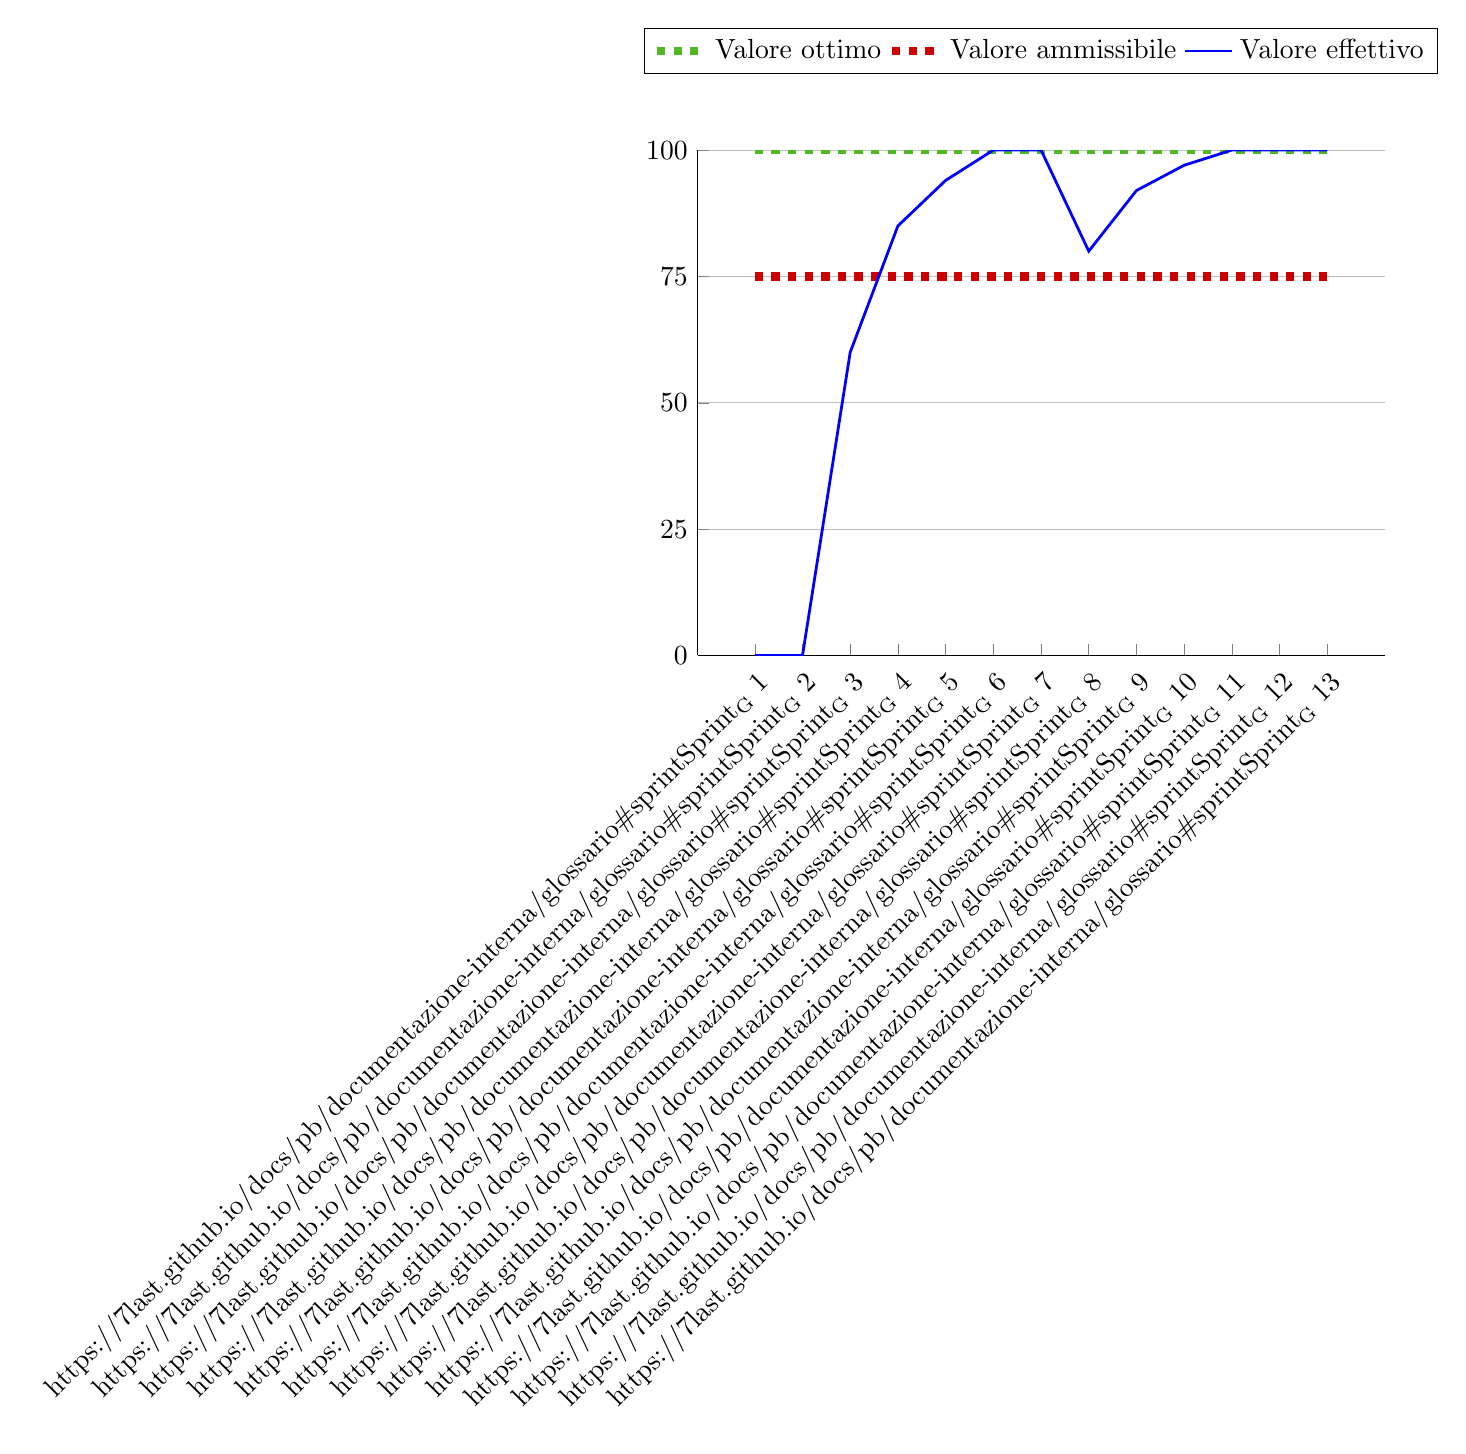
\begin{tikzpicture}
        \begin{axis}[
            width  = 0.85*\textwidth,
            height = 8cm,
            ymajorgrids = true,
            symbolic x coords={\href{https://7last.github.io/docs/pb/documentazione-interna/glossario\#sprint}{Sprint\textsubscript{G}} 1, \href{https://7last.github.io/docs/pb/documentazione-interna/glossario\#sprint}{Sprint\textsubscript{G}} 2, \href{https://7last.github.io/docs/pb/documentazione-interna/glossario\#sprint}{Sprint\textsubscript{G}} 3, \href{https://7last.github.io/docs/pb/documentazione-interna/glossario\#sprint}{Sprint\textsubscript{G}} 4, \href{https://7last.github.io/docs/pb/documentazione-interna/glossario\#sprint}{Sprint\textsubscript{G}} 5, \href{https://7last.github.io/docs/pb/documentazione-interna/glossario\#sprint}{Sprint\textsubscript{G}} 6, \href{https://7last.github.io/docs/pb/documentazione-interna/glossario\#sprint}{Sprint\textsubscript{G}} 7, \href{https://7last.github.io/docs/pb/documentazione-interna/glossario\#sprint}{Sprint\textsubscript{G}} 8, \href{https://7last.github.io/docs/pb/documentazione-interna/glossario\#sprint}{Sprint\textsubscript{G}} 9, \href{https://7last.github.io/docs/pb/documentazione-interna/glossario\#sprint}{Sprint\textsubscript{G}} 10, \href{https://7last.github.io/docs/pb/documentazione-interna/glossario\#sprint}{Sprint\textsubscript{G}} 11, \href{https://7last.github.io/docs/pb/documentazione-interna/glossario\#sprint}{Sprint\textsubscript{G}} 12, \href{https://7last.github.io/docs/pb/documentazione-interna/glossario\#sprint}{Sprint\textsubscript{G}} 13},
            xtick = data,
            ytick = {0, 25, 50, 75, 100},
            ymin=0, ymax=100,
            axis lines*=left,
            legend cell align=left,
            legend style={
                at={(0.5,1.15)},
                anchor=south,
                column sep=0.1ex,
                legend columns=3
            },
            xticklabel style={rotate=45, anchor=north east, yshift=0ex, xshift=0ex}
        ]
            \addplot[color=opt, style={dashed, line width=3pt}, mark=none] coordinates { % ottimo = 100
                (\href{https://7last.github.io/docs/pb/documentazione-interna/glossario\#sprint}{Sprint\textsubscript{G}} 1, 100)
                (\href{https://7last.github.io/docs/pb/documentazione-interna/glossario\#sprint}{Sprint\textsubscript{G}} 2, 100)
                (\href{https://7last.github.io/docs/pb/documentazione-interna/glossario\#sprint}{Sprint\textsubscript{G}} 3, 100)
                (\href{https://7last.github.io/docs/pb/documentazione-interna/glossario\#sprint}{Sprint\textsubscript{G}} 4, 100)
                (\href{https://7last.github.io/docs/pb/documentazione-interna/glossario\#sprint}{Sprint\textsubscript{G}} 5, 100)
                (\href{https://7last.github.io/docs/pb/documentazione-interna/glossario\#sprint}{Sprint\textsubscript{G}} 6, 100)
                (\href{https://7last.github.io/docs/pb/documentazione-interna/glossario\#sprint}{Sprint\textsubscript{G}} 7, 100)
                (\href{https://7last.github.io/docs/pb/documentazione-interna/glossario\#sprint}{Sprint\textsubscript{G}} 8, 100)
                (\href{https://7last.github.io/docs/pb/documentazione-interna/glossario\#sprint}{Sprint\textsubscript{G}} 9, 100)
                (\href{https://7last.github.io/docs/pb/documentazione-interna/glossario\#sprint}{Sprint\textsubscript{G}} 10, 100)
                (\href{https://7last.github.io/docs/pb/documentazione-interna/glossario\#sprint}{Sprint\textsubscript{G}} 11, 100)
                (\href{https://7last.github.io/docs/pb/documentazione-interna/glossario\#sprint}{Sprint\textsubscript{G}} 12, 100)
                (\href{https://7last.github.io/docs/pb/documentazione-interna/glossario\#sprint}{Sprint\textsubscript{G}} 13, 100)
            };
            \addplot[color=amm, style={dashed, line width=3pt}, mark=none] coordinates { % ammissibile = 75
                (\href{https://7last.github.io/docs/pb/documentazione-interna/glossario\#sprint}{Sprint\textsubscript{G}} 1, 75)
                (\href{https://7last.github.io/docs/pb/documentazione-interna/glossario\#sprint}{Sprint\textsubscript{G}} 2, 75)
                (\href{https://7last.github.io/docs/pb/documentazione-interna/glossario\#sprint}{Sprint\textsubscript{G}} 3, 75)
                (\href{https://7last.github.io/docs/pb/documentazione-interna/glossario\#sprint}{Sprint\textsubscript{G}} 4, 75)
                (\href{https://7last.github.io/docs/pb/documentazione-interna/glossario\#sprint}{Sprint\textsubscript{G}} 5, 75)
                (\href{https://7last.github.io/docs/pb/documentazione-interna/glossario\#sprint}{Sprint\textsubscript{G}} 6, 75)
                (\href{https://7last.github.io/docs/pb/documentazione-interna/glossario\#sprint}{Sprint\textsubscript{G}} 7, 75)
                (\href{https://7last.github.io/docs/pb/documentazione-interna/glossario\#sprint}{Sprint\textsubscript{G}} 8, 75)
                (\href{https://7last.github.io/docs/pb/documentazione-interna/glossario\#sprint}{Sprint\textsubscript{G}} 9, 75)
                (\href{https://7last.github.io/docs/pb/documentazione-interna/glossario\#sprint}{Sprint\textsubscript{G}} 10, 75)
                (\href{https://7last.github.io/docs/pb/documentazione-interna/glossario\#sprint}{Sprint\textsubscript{G}} 11, 75)
                (\href{https://7last.github.io/docs/pb/documentazione-interna/glossario\#sprint}{Sprint\textsubscript{G}} 12, 75)
                (\href{https://7last.github.io/docs/pb/documentazione-interna/glossario\#sprint}{Sprint\textsubscript{G}} 13, 75)
            };
            \addplot[color=blue, style={line width=1pt}, mark=none] coordinates { % RSI
                (\href{https://7last.github.io/docs/pb/documentazione-interna/glossario\#sprint}{Sprint\textsubscript{G}} 1, 0)
                (\href{https://7last.github.io/docs/pb/documentazione-interna/glossario\#sprint}{Sprint\textsubscript{G}} 2, 0)
                (\href{https://7last.github.io/docs/pb/documentazione-interna/glossario\#sprint}{Sprint\textsubscript{G}} 3, 60)
                (\href{https://7last.github.io/docs/pb/documentazione-interna/glossario\#sprint}{Sprint\textsubscript{G}} 4, 85)
                (\href{https://7last.github.io/docs/pb/documentazione-interna/glossario\#sprint}{Sprint\textsubscript{G}} 5, 94)
                (\href{https://7last.github.io/docs/pb/documentazione-interna/glossario\#sprint}{Sprint\textsubscript{G}} 6, 100)
                (\href{https://7last.github.io/docs/pb/documentazione-interna/glossario\#sprint}{Sprint\textsubscript{G}} 7, 100)
                (\href{https://7last.github.io/docs/pb/documentazione-interna/glossario\#sprint}{Sprint\textsubscript{G}} 8, 80)
                (\href{https://7last.github.io/docs/pb/documentazione-interna/glossario\#sprint}{Sprint\textsubscript{G}} 9, 92)
                (\href{https://7last.github.io/docs/pb/documentazione-interna/glossario\#sprint}{Sprint\textsubscript{G}} 10, 97)
                (\href{https://7last.github.io/docs/pb/documentazione-interna/glossario\#sprint}{Sprint\textsubscript{G}} 11, 100)
                (\href{https://7last.github.io/docs/pb/documentazione-interna/glossario\#sprint}{Sprint\textsubscript{G}} 12, 100)
                (\href{https://7last.github.io/docs/pb/documentazione-interna/glossario\#sprint}{Sprint\textsubscript{G}} 13, 100)
            };
            \legend{Valore ottimo, Valore ammissibile, Valore effettivo}
        \end{axis}
    \end{tikzpicture}
    \caption{Percentuale di stabilità dei requisiti}
\end{figure*}
%--------- FINE GRAFICO -----------%
\begin{flushleft}
\href{https://7last.github.io/docs/pb/documentazione-interna/glossario\#requirements-and-technology-baseline}{\textbf{RTB}\textsubscript{G}} \\
L'analisi del RSI mostra un forte incremento tra il secondo e il terzo \href{https://7last.github.io/docs/pb/documentazione-interna/glossario\#sprint}{sprint\textsubscript{G}}, segnalando un'intensa attività di revisione e aggiustamento dei requisiti. Nei due \href{https://7last.github.io/docs/pb/documentazione-interna/glossario\#sprint}{sprint\textsubscript{G}} successivi, il RSI si stabilizza, indicando una riduzione delle modifiche e una maggiore stabilità dei requisiti. Questo andamento riflette un'efficace fase iniziale di consolidamento dei requisiti seguita da una stabilizzazione che facilita l'implementazione del progetto. \\
\href{https://7last.github.io/docs/pb/documentazione-interna/glossario\#product-baseline}{\textbf{PB}\textsubscript{G}} \\
Dal grafico si può notare come i requisiti abbiano subito alcune modifiche in corrispondenza dell'ottavo \href{https://7last.github.io/docs/pb/documentazione-interna/glossario\#sprint}{sprint\textsubscript{G}} (e successivi). Questo è dovuto alla necessità di apportare alcune modifiche ai requisiti in seguito ai consigli ricevuti dal professor Cardin durante la revisione \href{https://7last.github.io/docs/pb/documentazione-interna/glossario\#requirements-and-technology-baseline}{RTB\textsubscript{G}}, oltre ad alcune variazioni concordate con il \href{https://7last.github.io/docs/pb/documentazione-interna/glossario\#proponente}{proponente\textsubscript{G}} su alcune funzionalità del prodotto. Questo ha permesso di migliorare la qualità del prodotto e di garantire una maggiore soddisfazione del \href{https://7last.github.io/docs/pb/documentazione-interna/glossario\#proponente}{proponente\textsubscript{G}}.
\end{flushleft}
